%%%---PREAMBLE---%%%%%%%%%%%%%%%%%%%%%%%%%%%%
% \documentclass[oneside,12pt,final]{sty/ucthesis-CA2012}
\documentclass[oneside,12pt,final]{sty/ucthesis-CA2012}
\pdfoutput=1

%--- Packages ---------------------------------------------------------
\usepackage[lofdepth,lotdepth,caption=false]{subfig}
\usepackage{fancyhdr}
\usepackage{hyperref}
\usepackage{amsmath, amssymb, graphicx}
\usepackage{xspace}
\usepackage{braket}
\usepackage{color}
\usepackage{setspace}
\usepackage{bibentry}
\usepackage{lipsum}
\usepackage{commath}
\usepackage{slashed}
\usepackage{todonotes}
\usepackage{multirow}
%\usepackage{subfigure} (Subfigure package clashes with another package)

% https://tex.stackexchange.com/questions/167660/subsection-not-showing-up-in-toc
\setcounter{tocdepth}{3}
\setcounter{secnumdepth}{3}

%---New Definitions and Commands------------------------------------------------------
\def\p{\partial}
\def\im{\mrm{im}}
\def\Tr{\mrm{Tr}}
\def\Z{\mbb{Z}}
\def\R{\mbb{R}}
\def\C{\mbb{C}}
\def\half{\frac{1}{2}}
\def\filler{\phantom{fillerfillerfiller}}
\newcommand{\mbb}[1]{\mathbb{#1}}
\newcommand{\mrm}[1]{\mathrm{#1}}
\newcommand{\mcal}[1]{\mathcal{#1}}
\newcommand{\mbf}[1]{\mathbf{#1}}
\newcommand{\ph}[1]{\phantom{#1}}
\newcommand{\udten}[3]{#1^{#2}_{\ph{#2}#3}}
\newcommand{\duten}[3]{#1^{\ph{#2}#3}_{#2}}
\newcommand{\sthirteen}{\ensuremath{\sqrt{\mathrm{s}}=13~\mathrm{TeV}}\xspace}
\newcommand{\ifb}{fb\ensuremath{{}^{-1}}}
\newcommand{\fbinv}{\ifb}

\newcommand{\sslumi}{137\fbinv}
\newcommand{\Njets}{\ensuremath{N_\text{jets}}\xspace}
\newcommand{\Nbjets}{\ensuremath{N_\mathrm{b}}\xspace}
\newcommand{\Nleps}{\ensuremath{N_\ell}\xspace}
\newcommand{\ttbar}{\ensuremath{t\bar{t}}\xspace}
\newcommand{\tttt}{\ensuremath{\ttbar\ttbar}\xspace}
\newcommand{\smft}{SM \ensuremath{\ttbar\ttbar}\xspace}
\newcommand{\ttZ}{\ensuremath{\ttbar Z}\xspace}
\newcommand{\ttW}{\ensuremath{\ttbar W}\xspace}
\newcommand{\xsectttt}{\ensuremath{\sigma(pp\to\tttt})\xspace}
\newcommand{\unit}[1]{\ensuremath{\text{\,#1}}\xspace}
\newcommand{\PQu}{u\xspace}
\newcommand{\PQd}{d\xspace}
\newcommand{\PQs}{s\xspace}
\newcommand{\PQc}{c\xspace}
\newcommand{\PQb}{b\xspace}
\newcommand{\PQt}{t\xspace}
\newcommand{\PQq}{q\xspace}
\newcommand{\cPq}{\PQq}
\newcommand{\cPqt}{\PQt}
\newcommand{\cPqb}{\PQb}
\newcommand{\cPqc}{\PQc}
\newcommand{\cPqs}{\PQs}
\newcommand{\PW}{W\xspace}
\newcommand{\PZ}{Z\xspace}
\newcommand{\PH}{H\xspace}
\newcommand{\PSA}{A\xspace}
\newcommand{\Pp}{p}
\newcommand{\ttH}{\ensuremath{\ttbar\PH}\xspace}
\newcommand{\tHW}{\ensuremath{\PQt\PH\PW}\xspace}
\newcommand{\tHq}{\ensuremath{\PQt\PH\PQq}\xspace}
\newcommand{\ttA}{\ensuremath{\ttbar\PSA}\xspace}
\newcommand{\tAW}{\ensuremath{\PQt\PSA\PW}\xspace}
\newcommand{\tAq}{\ensuremath{\PQt\PSA\PQq}\xspace}
\newcommand{\pt}{\ensuremath{p_{\mathrm{T}}}\xspace}
\newcommand{\ET}{\ensuremath{E_{\mathrm{T}}}\xspace}
\newcommand{\HT}{\ensuremath{H_{\mathrm{T}}}\xspace}
\newcommand{\mT}{\ensuremath{m_{\mathrm{T}}}\xspace}
\newcommand{\GeV}{\ensuremath{\text{GeV}}\xspace}
\newcommand{\TeV}{\ensuremath{\text{TeV}}\xspace}
\newcommand{\ETm}{\ensuremath{E_{\mathrm{T}}^{\text{miss}}}\xspace}
\newcommand{\ptvecmiss}{\ensuremath{{\vec p}_{\mathrm{T}}^{\kern1pt\text{miss}}}\xspace}
\newcommand{\ptmiss}{\ensuremath{\pt^\text{miss}}\xspace}
\newcommand{\CL}{\ensuremath{\text{CL}}\xspace}
\newcommand{\CLs}{\ensuremath{\text{CL}_\text{s}}\xspace}
\newcommand{\CLsb}{\ensuremath{\text{CL}_\text{s+b}}\xspace}
\newcommand{\cPZpr}{\ensuremath{Z^\prime}\xspace}
\newcommand{\MTmin}{\ensuremath{\mT^{\text{min}}}\xspace}
\newcommand{\mtmin}{\MTmin}

\newcommand{\NA}{--}

\newcommand{\gluino}{\ensuremath{\tilde{g}}\xspace}
\newcommand{\susyq}{\ensuremath{\tilde{q}}\xspace}
\newcommand{\susytop}{\ensuremath{\tilde{t}}\xspace}
\newcommand{\susytopone}{\ensuremath{\tilde{t}_1}\xspace}
\newcommand{\susytoptwo}{\ensuremath{\tilde{t}_2}\xspace}
\newcommand{\ptcorr}{\ensuremath{\pt^\text{corr}}\xspace}
\newcommand{\nisrjet}{\ensuremath{N_\mathrm{J}^\text{ISR}}\xspace}
\newcommand{\sbottomone}{\ensuremath{\tilde{b}_1}\xspace}
\newcommand{\lsp}{\ensuremath{\tilde{\chi}_1^0}\xspace}
\newcommand{\neutralinotwo}{\ensuremath{\tilde{\chi}_2^0}\xspace}
\newcommand{\chiminus}{\ensuremath{\tilde{\chi}_1^{-}}\xspace}
\newcommand{\chiplus}{\ensuremath{\tilde{\chi}_1^{+}}\xspace}
\newcommand{\chiplmin}{\ensuremath{\tilde{\chi}_1^{\pm}}\xspace}
\newcommand{\Totttt}{\ensuremath{\mathrm{T1\PQt\PQt\PQt\PQt}}\xspace}
\newcommand{\Tftttt}{\ensuremath{\mathrm{T5\PQt\PQt\PQt\PQt}}\xspace}
\newcommand{\Tfttcc}{\ensuremath{\mathrm{T5\PQt\PQt\PQc\PQc}}\xspace}
\newcommand{\TfqqqqWZ}{\ensuremath{\mathrm{T5\PQq\PQq\PQq\PQq\PW\PZ}}\xspace}
\newcommand{\TfqqqqWW}{\ensuremath{\mathrm{T5\PQq\PQq\PQq\PQq\PW\PW}}\xspace}
\newcommand{\TsttWW}{\ensuremath{\mathrm{T6\PQt\PQt\PW\PW}}\xspace}
\newcommand{\TsttHZ}{\ensuremath{\mathrm{T6\PQt\PQt\PH\PZ}}\xspace}
\newcommand{\TfttbbWW}{\ensuremath{\mathrm{T5\PQt\PQt\PQb\PQb\PW\PW}}\xspace}
\newcommand{\Totbs}{\ensuremath{\mathrm{T1\PQt\PQb\PQs}}\xspace}
\newcommand{\ToqqqqL}{\ensuremath{\mathrm{T1\PQq\PQq\PQq\PQq L}}\xspace}

\newcommand{\miniiso}{\ensuremath{I_\mathrm{mini}}\xspace}
\newcommand{\ptratio}{\ensuremath{\pt^\text{ratio}}\xspace}
\newcommand{\ptrel}{\ensuremath{\pt^\text{rel}}\xspace}

\newcommand{\mytodo}[1]{\todo[inline, color=red!40]{#1}}

% \def\dsp{\def\baselinestretch{1.0}\large\normalsize} % FIXME remove this line when compiling final thesis
% https://stackoverflow.com/questions/1465665/passing-command-line-arguments-to-latex-document/1466610#1466610
% \ifdefined\myownflag
    % \def\dsp{\def\baselinestretch{1.0}\large\normalsize}
% \fi
% uncomment ifdefined, fi lines to go back to double space

%---Set Margins ------------------------------------------------------
\setlength\oddsidemargin{0.25 in} \setlength\evensidemargin{0.25 in} \setlength\textwidth{6.25 in} \setlength\textheight{8.50 in}
\setlength\footskip{0.25 in} \setlength\topmargin{0 in} \setlength\headheight{0.25 in} \setlength\headsep{0.25 in}

%%%---DOCUMENT---%%%%%%%%%%%%%%%%%%%%%%%%%%%%
\begin{document}

%=== Preliminary Pages ============================================
\begin{frontmatter}
	%%%%%%%%%%%%%%%%%%%%%%%%%%%
% TITLE PAGE INFORMATION %
%%%%%%%%%%%%%%%%%%%%%%%%%%%


\title{Methodological observation of the sociometrical behavior tendencies of pre-maturated isolates}

\author{David McAlister Barry}

%%%%%%%%%%%%%%%%%%%%%%%%%%%%%%%%%%
% DECLARATIONS FOR FRONT MATTER %
%%%%%%%%%%%%%%%%%%%%%%%%%%%%%%%%%%
\report{Dissertation} \degree{Doctor of Philosophy} \degreemonth{Month} \degreeyear{2018}
\defensemonth{March} % should be one of the following: March, 
\defenseyear{2018}

\chair{Professor Charles McThornbody}  % this is your advisor
\othermemberA{Professor Russell Hammond} % This is a member of your committee 
\othermemberB{Professor Alfred Alfredo} % This is a member of your committee 
\othermemberC{Professor Jackmerius Tacktheritrix} % This is a member of your committee (if your department requires 4 members)
\numberofmembers{4} % should match the number of entries above (chair + othermembers)

\field{Electrical and Computer Engineering}
\campus{Santa Barbara}


%\title{{ University of California \\ Santa Barbara} \linebreak \\  Ph.D. Dissertation}
%\author{Tom\'as Andrade}
%\date{2012}

	\maketitle
	\approvalpage
	\copyrightpage
	\begin{acknowledgements}

Acknowledgements Here.  

\end{acknowledgements} 
	\begin{vitae}
\addcontentsline{toc}{chapter}{Curriculum Vitae}

\begin{vitaesection}{Education}
\vspace{-0.1cm}
\item [2019] Ph.D. in Physics (Expected), University of California, Santa Barbara.
\item [2017] M.Sc. in Physics, University of California, Santa Barbara.
\item [2014] B.Sc. in Physics, Texas A\&M University, College Station, TX.
\end{vitaesection}

\textbf{Publications}

% \nobibliography*
% \begin{itemize}
%     \item \bibentry{GAN:LHC2019} % http://inspirehep.net/record/1714018
%     \item \bibentry{CMS:myTOPRun2PAS} % http://inspirehep.net/record/1726177
%     \item \bibentry{CMS:mySUSRun2PAS} % http://inspirehep.net/record/1726691
%     \item \bibentry{CMS:myTOP2016} % http://inspirehep.net/record/1633423
%     \item \bibentry{CMS:mySUS2016} % http://inspirehep.net/record/1594731
% \end{itemize}


    \begin{itemize}
        \item B. Hashemi, N. Amin, K. Datta, D. Olivito, and M. Pierini, \textit{LHC analysis-specific datasets with Generative Adversarial Networks} [\href{https://arxiv.org/abs/1901.05282}{arXiv:1901.0528}] \textbf{In progress}
        \item CMS Collaboration, \textit{Search for standard model production of four top quarks in final states with same-sign and multiple leptons in proton-proton collisions at \sthirteen} 
            [\href{http://inspirehep.net/record/1726177}{PAS TOP-18-003}] \textbf{In progress}
        \item CMS Collaboration, \textit{Search for physics beyond the standard model in events with two same-sign leptons or at least three leptons and jets in proton-proton collisions at \sthirteen} 
            [\href{http://inspirehep.net/record/1726691}{PAS SUS-19-008}] \textbf{In progress}
        \item CMS Collaboration, \textit{Search for standard model production of four top quarks with same-sign and multilepton final states in proton-proton collisions at \sthirteen},
            \textit{Eur. Phys. J.} \textbf{C78} (2018) 
            [\href{https://arxiv.org/abs/1710.1061}{arXiv:1710.1061}]
        \item CMS Collaboration, \textit{Search for physics beyond the standard model in events with two leptons of same sign, missing transverse momentum, and jets in proton-proton collisions at \sthirteen}
            \textit{Eur. Phys. J.} \textbf{C77} (2017) 
            [\href{https://arxiv.org/abs/1704.07323}{arXiv:1704.07323}]
    \end{itemize}

\end{vitae}

	\begin{abstract}
\addcontentsline{toc}{chapter}{Abstract}

Two related searches for Standard Model and beyond the Standard Model physics
    with a final state containing a pair of same-charged leptons and jets are
    performed using a sample of \sthirteen data corresponding to an integrated
    luminosity of 137~\ifb, collected by the CMS detector between 2016 and
    2018. The first inclusive search observes no excess above the Standard
    Model and thus places constraints on R-parity violating and R-parity
    conserving supersymmetric models with pair production of gluinos and
    squarks.  Gluino masses are excluded up to 2.1 TeV, while top and bottom
    squarks are excluded up to 0.9 TeV.  The second search measures the
    cross-section of the production of four top quarks within the Standard
    Model using both cut-based and multivariate approaches.  The observed
    (expected) significance of the multivariate approach is 2.6 (2.7) standard
    deviations, with a measured cross-section of $12.6^{+5.8}_{-5.2}$ fb,
    consistent with the Standard Model prediction of $12.0^{+2.2}_{-2.5}$ fb.
    These results are translated into constraints on the Yukawa coupling of the
    top quark, as well as constraints on heavy scalar or pseudoscalar
    production in a type II 2HDM scenario.

%\abstractsignature
\end{abstract}



	\tableofcontents
\end{frontmatter}

\begin{mainmatter}

%---Set Headers and Footers ------------------------------------------------------
\pagestyle{fancy}
\renewcommand{\chaptermark}[1]{\markboth{{\sf #1 \hspace*{\fill} Chapter~\thechapter}}{} }
\renewcommand{\sectionmark}[1]{\markright{ {\sf Section~\thesection \hspace*{\fill} #1 }}}
\fancyhf{}

\makeatletter \if@twoside \fancyhead[LO]{\small \rightmark} \fancyhead[RE]{\small\leftmark} \else \fancyhead[LO]{\small\leftmark}
\fancyhead[RE]{\small\rightmark} \fi

\def\cleardoublepage{\clearpage\if@openright \ifodd\c@page\else
  \hbox{}
  \vspace*{\fill}
  \begin{center}
    This page intentionally left blank
  \end{center}
  \vspace{\fill}
  \thispagestyle{plain}
  \newpage
  \fi \fi}
\makeatother
\fancyfoot[c]{\textrm{\textup{\thepage}}} % page number
\fancyfoot[C]{\thepage}
\renewcommand{\headrulewidth}{0.4pt}

\fancypagestyle{plain} { \fancyhf{} \fancyfoot[C]{\thepage}
\renewcommand{\headrulewidth}{0pt}
\renewcommand{\footrulewidth}{0pt}}

\begin{enumerate}

	\item Chapter 1 -- Introduction
    \begin{enumerate}
    	\item Standard model
        \begin{enumerate}
            \item Describe SM
            \item Table of particles
        \end{enumerate}
    	\item Beyond the standard model
        \begin{enumerate}
            \item Issues with SM
            \begin{enumerate}
                \item Higgs mass/hierarchy problem
                \item Dark matter/neutrino masses/matter asymmetry
            \end{enumerate}
            \item SUSY
            \item LHC
            \item CMS
        \end{enumerate}
    \end{enumerate}

	\item Chapter 2 -- Same-sign final state
    \begin{enumerate}
    	\item SS signature/BSM intro
        \begin{enumerate}
            \item SM xsecs plot
            \item SUSY xsecs, SUSY diagrams + descriptions
            \item SM tttt diagrams, BSM tttt diagrams (2HDM)
        \end{enumerate}
    	\item Short description of backgrounds
        \begin{enumerate}
            \item 1-2 paragraphs about main backgrounds
        \end{enumerate}
    \end{enumerate}

	\item Chapter 3 -- Objects and variables
    \begin{enumerate}
    	\item Jets, MET
        \begin{enumerate}
            \item Jet ID, JEC
            \item MET
            \item B-tag, performance plot
        \end{enumerate}
    	\item Leptons
        \begin{enumerate}
            \item ID
            \item Isolation
        \end{enumerate}
    	\item Trigger
    	\item Key variables
        \begin{enumerate}
            \item mtmin, njets
            \item nleps, ...
        \end{enumerate}
    	\item Event-level BDT
    	\item Signal regions
    \end{enumerate}


	\item Chapter 4 -- Background estimation
    \begin{enumerate}
    	\item Rares
    	\item Fakes
    	\item Flips
    	\item Uncertainties, systematics
    \end{enumerate}

	\item Chapter 5 -- Results and interpretations
    \begin{enumerate}
    	\item Results
        \begin{enumerate}
            \item SR plots, tttt
        \end{enumerate}
    	\item SUSY interpretations
        \begin{enumerate}
            \item SMS exclusions
            \item Model-independent limits
        \end{enumerate}
    	\item BSM tttt interpetations
    \end{enumerate}


	\item Chapter 6 -- Summary and conclusions

\end{enumerate}

\chapter{Introduction}

\begin{section}{Info}
Some facts


The results presented in this thesis correspond to the published results in Refs.~\cite{CMS:myTOPRun2,CMS:mySUSRun2PAS,CMS:myTOP2016,CMS:mySUS2016}.

\end{section}
 % Introduction
\chapter{Same-sign dilepton final state}
\label{chap:ssdl}

Almost every new (or rare SM) physics analysis relies on a ``killer'' variable
or technique
to differentiate signal from background and increase the signal-to-noise
ratio to a level that is conducive to further interpretation.
The technique used in this thesis exploits the fact that seeing a pair of leptons
with the same charge as a product of proton-proton collision processes
(e.g., $\PW$/$\PZ$ production, QCD) is very, very rare,
but is quite common in scenarios of new (or rare SM) physics.

We start by examining the rare production of four top quarks (\tttt) in the SM,
as SUSY processes follow
similar patterns and will be dicussed in more detail in the subsequent section.
The four top quarks of SM \tttt will each decay into a \PQb quark and \PW boson.
A \PW boson decays into a charged lepton and matching neutrino 
($e\bar\nu_e$, $\mu\bar\nu_\mu$, $\tau\bar\nu_\tau$) with approximately 1/3 probability.
For four \PW bosons ($\PW^+\PW^+\PW^-\PW^-$), the lepton multiplicities and characteristics are summarized in
Fig~\ref{fig:fourtoppie}. Up to 12\% of SM \tttt can be selected by requiring
a same-sign (SS) dilepton ($e$ or $\mu$) in the final state, which includes the
leptonic branching ratio of $\tau$ to $e$ or $\mu$. 

Turning to background SM processes, to first order, requiring two leptons
(SS or not) directly eliminates QCD processes  with only quarks/gluons (u, d, s, c, b, g) in the final state.
Figure~\ref{fig:SMxsecs} summarizes
CMS measurements of many other SM processes.
Three of the highest cross section processes 
are $\PW$, $\PZ$, and $\ttbar$, which give one lepton or two opposite sign leptons,
and would also be eliminated by requiring SS dileptons.
In fact, continuing down the mountain of processes, the first process that can give prompt
SS dileptons is $\PW\PZ$. Thus, the SS dilepton selection is an effective
``cut'' that rejects processes above $\mathrm{O}(10)\unit{pb}$. Compared to many other
search strategies, which exploit extreme event kinematics, the SS dilepton selection allows probing softer
events with less transverse momenta and missing transverse energy.




\begin{figure}[!hbtp]
\centering
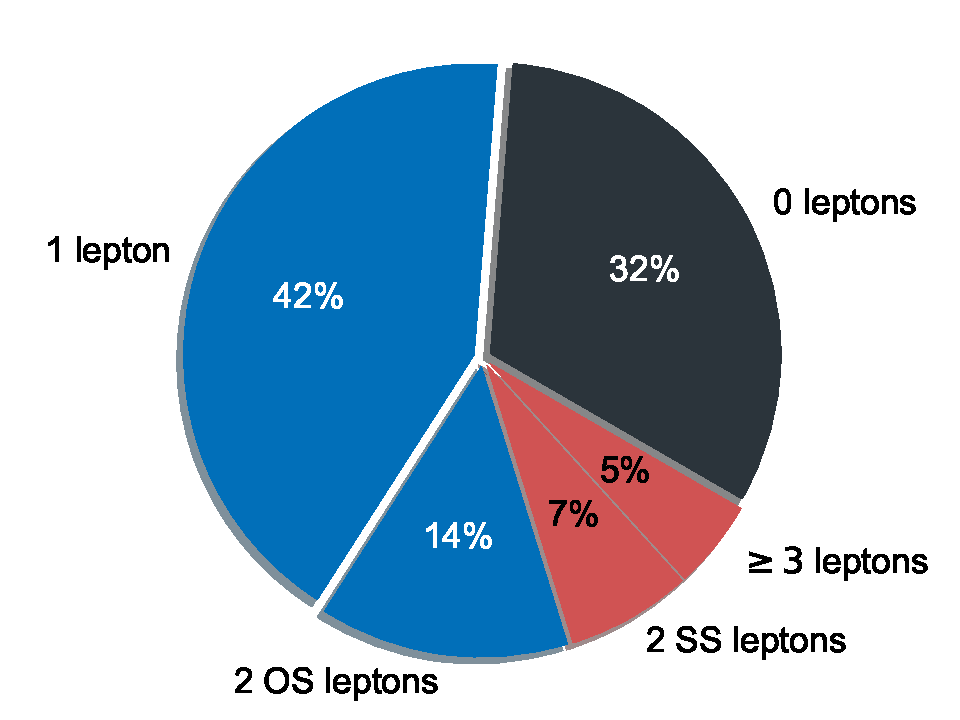
\includegraphics[width=.50\textwidth]{figs/misc/fourtopdecay_pie.pdf} \\
\caption{Lepton multiplicities of four $\PW$ final states.}
\label{fig:fourtoppie}
\end{figure}

\begin{figure}[!hbtp]
\centering
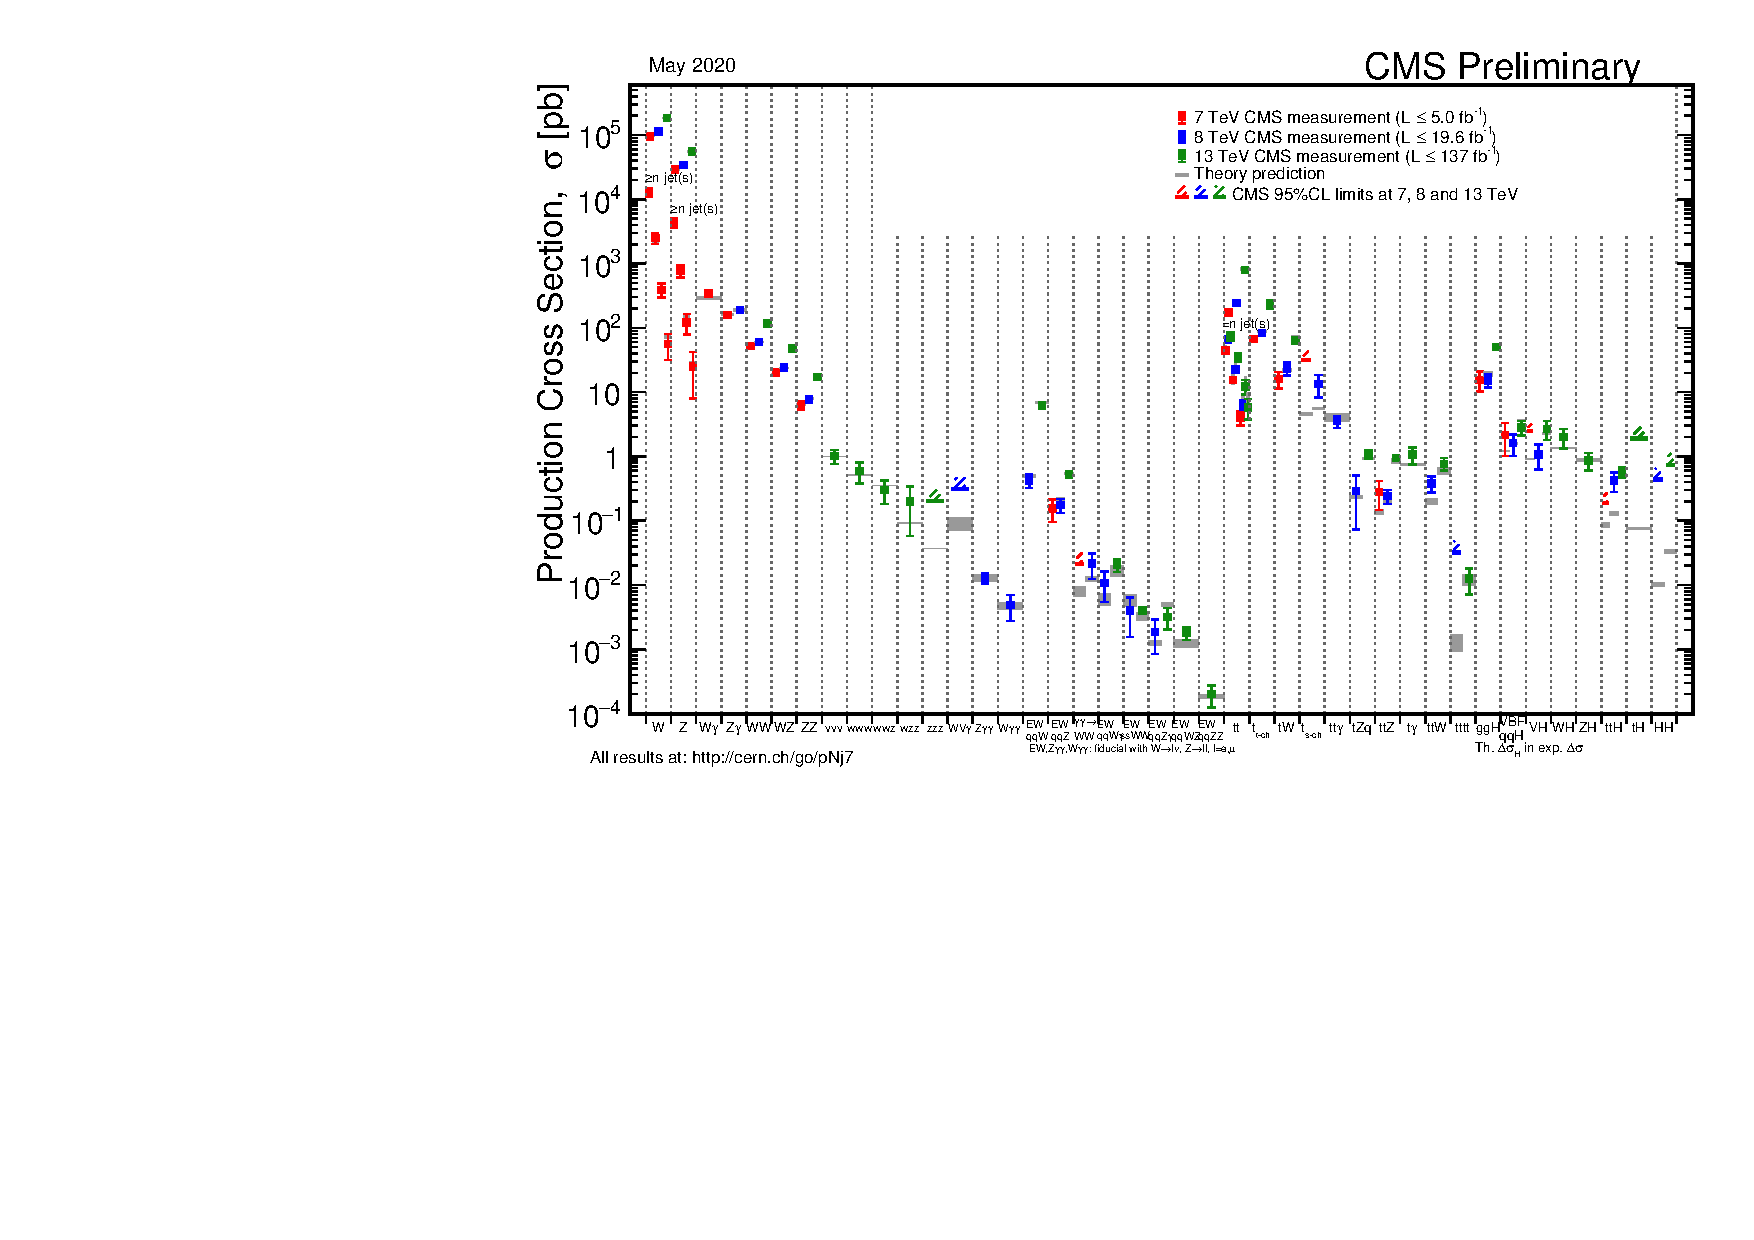
\includegraphics[width=.95\textwidth]{figs/misc/sm_xsecs.pdf} \\
\caption{Summary of SM cross section measurements at CMS~\cite{CMS:SMxsecs}.
(Spoiler alert: the results presented later in this thesis correspond to one
of the points in this plot!)
}
\label{fig:SMxsecs}
\end{figure}

\FloatBarrier

\section{SUSY processes}


Many SUSY models with strong pair production mechanisms result in
final states with a number of leptons, ideal for SS final states.
Here, we consider simplified models of SUSY with a reduced number of
parameters~\cite{ref:CMS:SMS}, where signal model hypotheses are specified
by a production and decay process with one or two SUSY particle masses
fixed to particular masses that are ``scanned'' over.
Cross sections of pair production models with gluinos and squarks 
are shown in Fig.~\ref{fig:susy_xsecs}, and are as low as a few \fbinv 
for gluino/squark masses between 1.5\TeV and 2\TeV.

\begin{figure}[htb!]
    \centering
    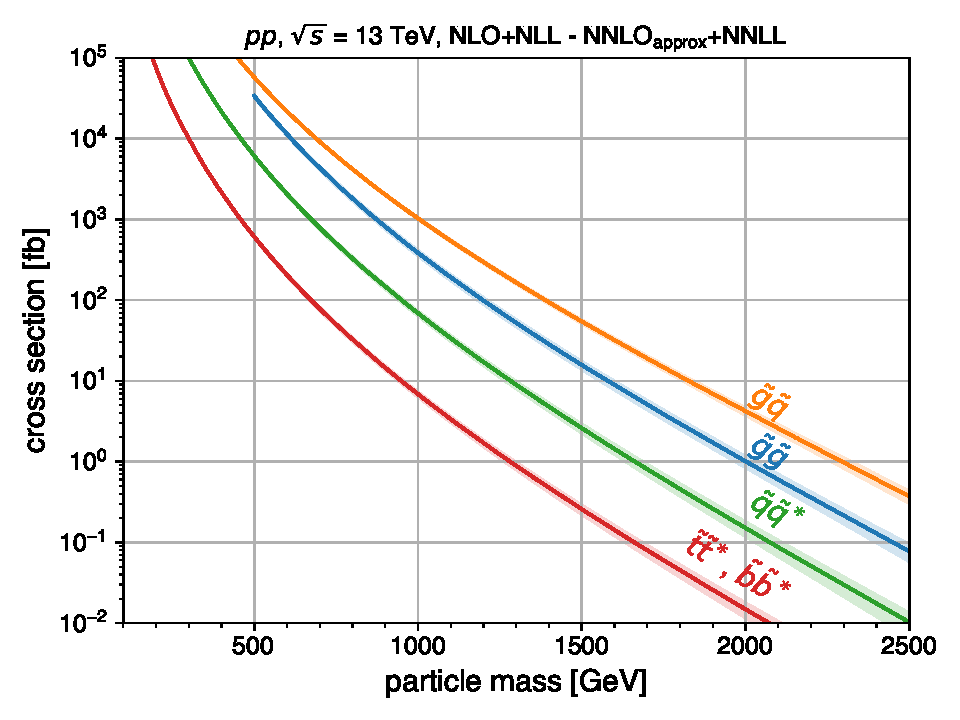
\includegraphics[width=0.85\textwidth]{figs/ssan/plot_susy_xsecs}
\caption{Strong production cross sections for SUSY processes at the LHC. Calculations from \cite{THEORY:SUSYxsecs}.}
\label{fig:susy_xsecs}
\end{figure}

Gluino pair production models giving rise to signatures with up to four \cPqb\
quarks and \PW\ bosons are shown in Fig.~\ref{fig:susy_diag_set1}. In
these models, the gluino decays to the lightest squark ($\gluino \to \susyq
\cPq$), which then decays to same-flavor ($\susyq \to \cPq \lsp$) or
different-flavor ($\susyq \to \cPq' \chiplmin$) quarks. The chargino
($\chiplmin$) decays to a \PW\ boson and a neutralino ($\lsp$) via $\chiplmin
\to \PW^{\pm} \lsp$, where the \lsp is taken to be the lightest stable SUSY (LSP)
particle and is not directly detectable.

The first scenario, displayed in Fig.~\ref{fig:susy_diag_set1}a and denoted
\Totttt, includes an off-shell top squark ($\susytop$) leading to a
three-body decay of the gluino, $\gluino \to \ttbar\lsp$, and resulting in events
with four \PW\ bosons and four \cPqb\ quarks. This topology is thus similar
to SM \tttt with the addition of missing energy from the invisible LSP.
Figure~\ref{fig:susy_diag_set1}b presents a similar model (\TfttbbWW) but where
the gluino decay results in a chargino that decays into a neutralino
and a \PW\ boson. The model shown in Fig.~\ref{fig:susy_diag_set1}c (\Tftttt)
is identical to \Totttt except that the intermediate top squark is on-shell.
The mass splitting between the $\susytop$ and the \lsp is taken to be
$m_{\susytop} - m_{\lsp} = m_{\cPqt}$, where $m_{\cPqt}$ is the top quark
mass. This mass splitting corresponds to a challenging region of parameter
space for the observation of the $\susytop \to \cPqt \lsp$ decay. The model
of Fig.~\ref{fig:susy_diag_set1}d (\Tfttcc) is identical to 
\Tftttt except that the $\susytop$ decay involves a \PQc quark. In
Fig.~\ref{fig:susy_diag_set1}e, the process includes a virtual
light-flavor squark, leading to three-body decays of $\gluino \to \cPq \cPq'
\chiplmin$ or $\gluino \to \cPq \cPq' \neutralinotwo$, with a resulting
signature of two \PW\ bosons, two \PZ\ bosons, or one of each (the case shown
in Fig.~\ref{fig:susy_diag_set1}e), and four light-flavor jets. This model,
\TfqqqqWZ, with a resulting signature of one \PW\ boson and one \PZ\ boson,
is considered separately for two different assumptions of the chargino mass,
$m_{\chiplmin} = 0.5(m_{\gluino} + m_{\lsp})$, and $m_{\chiplmin} =
m_{\lsp}+20 \GeV$, producing on- and off-shell bosons, respectively. The
model is also considered with the assumption of decays to two \PW\ bosons (\TfqqqqWW).

Figure~\ref{fig:susy_diag_set2}a shows a model of bottom squark production and decay
via $\sbottomone \to \cPqt \chiplmin$, giving two \cPqb\
quarks and four \PW\ bosons. This model, \TsttWW, is considered as a function
of the the lightest bottom squark, $\sbottomone$, and \chiplmin masses. The
\lsp mass is fixed at 50\GeV, which results in two off-shell \PW\ bosons 
when the \chiplmin mass is less than approximately
130\GeV. Figure~\ref{fig:susy_diag_set2}b displays the \TsttHZ model
with top squark pair production and a subsequent decay of
$\susytoptwo\to\susytopone\PH/\PZ$, with $\susytopone \to \cPqt\lsp$,
producing signatures with two \PH\ bosons, two \PZ\ bosons, or one of each.
In this model the \lsp mass is fixed such that
$m(\susytopone)-m(\lsp)=m_{\cPqt}$.

The R parity violating (RPV) decays considered in the SUSY analysis are \ToqqqqL
(Fig.~\ref{fig:susy_diag_set3}a) and \Totbs (Fig.~\ref{fig:susy_diag_set3}b). 
Unlike the previously discussed processes, these RPV processes do not have a stable
LSP.
In \ToqqqqL, the gluino decays to the lightest squark ($\gluino \to \susyq
\cPq$), which decays to a quark ($\susyq \to \cPq \lsp$)
with an off shell $\lsp$ decaying into two quarks and a charged
lepton, giving rise to a prompt 5-body decay of the gluino. In the \Totbs model, the
gluinos each decay into three different SM quarks ($\PQt$, $\PQb$, and $\PQs$).

\begin{figure}[htb!]
    \centering
    \subfloat[T1tttt]{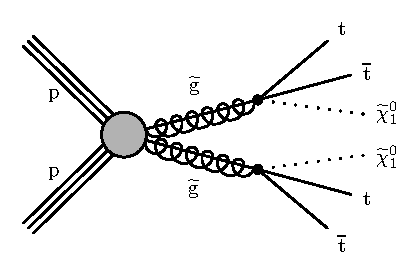
\includegraphics[width=0.48\textwidth]{figs/ssp/diag_T1tttt}}
    \subfloat[T5ttbbWW]{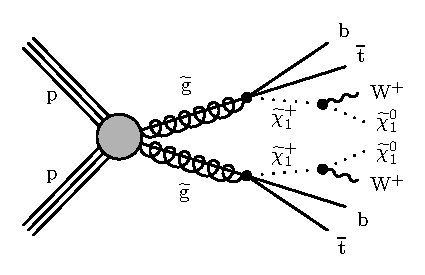
\includegraphics[width=0.48\textwidth]{figs/ssp/diag_T5ttbbWW}} \\
    \subfloat[T5tttt]{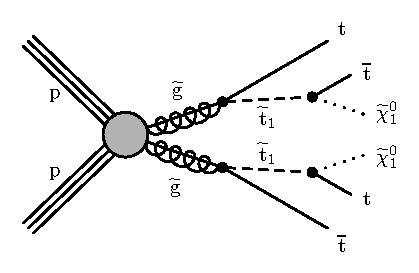
\includegraphics[width=0.48\textwidth]{figs/ssp/diag_T5tttt}}
    \subfloat[T5ttcc]{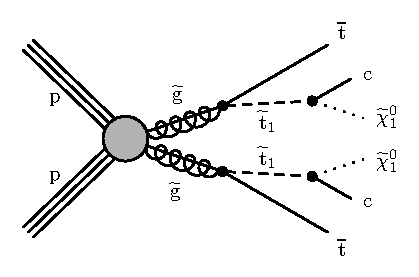
\includegraphics[width=0.48\textwidth]{figs/ssp/diag_T5ttcc}} \\
    \subfloat[T5qqqqWZ]{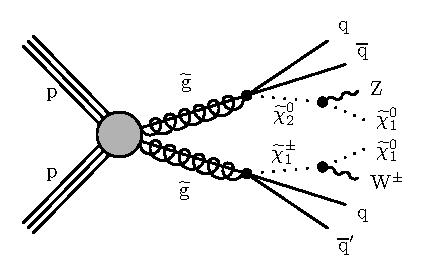
\includegraphics[width=0.48\textwidth]{figs/ssp/diag_T5qqqqWZ}}
\caption{Diagrams illustrating the simplified RPC SUSY models with gluino production considered in this analysis.}
\label{fig:susy_diag_set1}
\end{figure}

\begin{figure}[htb!]
    \centering
    \subfloat[T6ttWW]{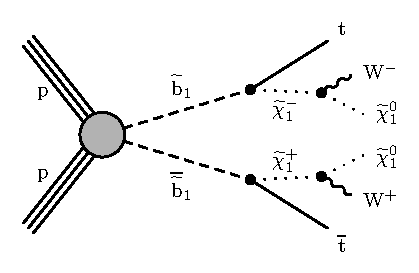
\includegraphics[width=0.48\textwidth]{figs/ssp/diag_T6ttWW}}
    \subfloat[T6ttHZ]{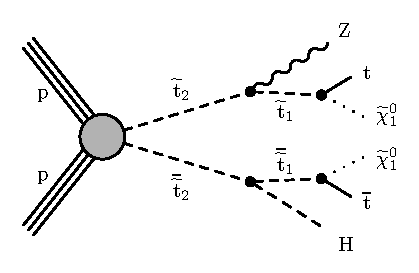
\includegraphics[width=0.48\textwidth]{figs/ssp/diag_T6ttHZ}} \\
\caption{Diagrams illustrating the simplified RPC SUSY models with squark production considered in this analysis.}
\label{fig:susy_diag_set2}
\end{figure}

\begin{figure}[htb!]
    \centering
    \subfloat[T1qqqqL]{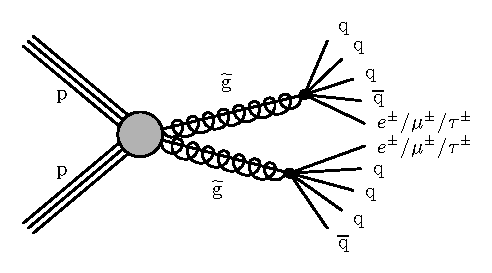
\includegraphics[width=0.53\textwidth]{figs/ssp/diag_T1qqqqL}}
    \subfloat[T1tbs]{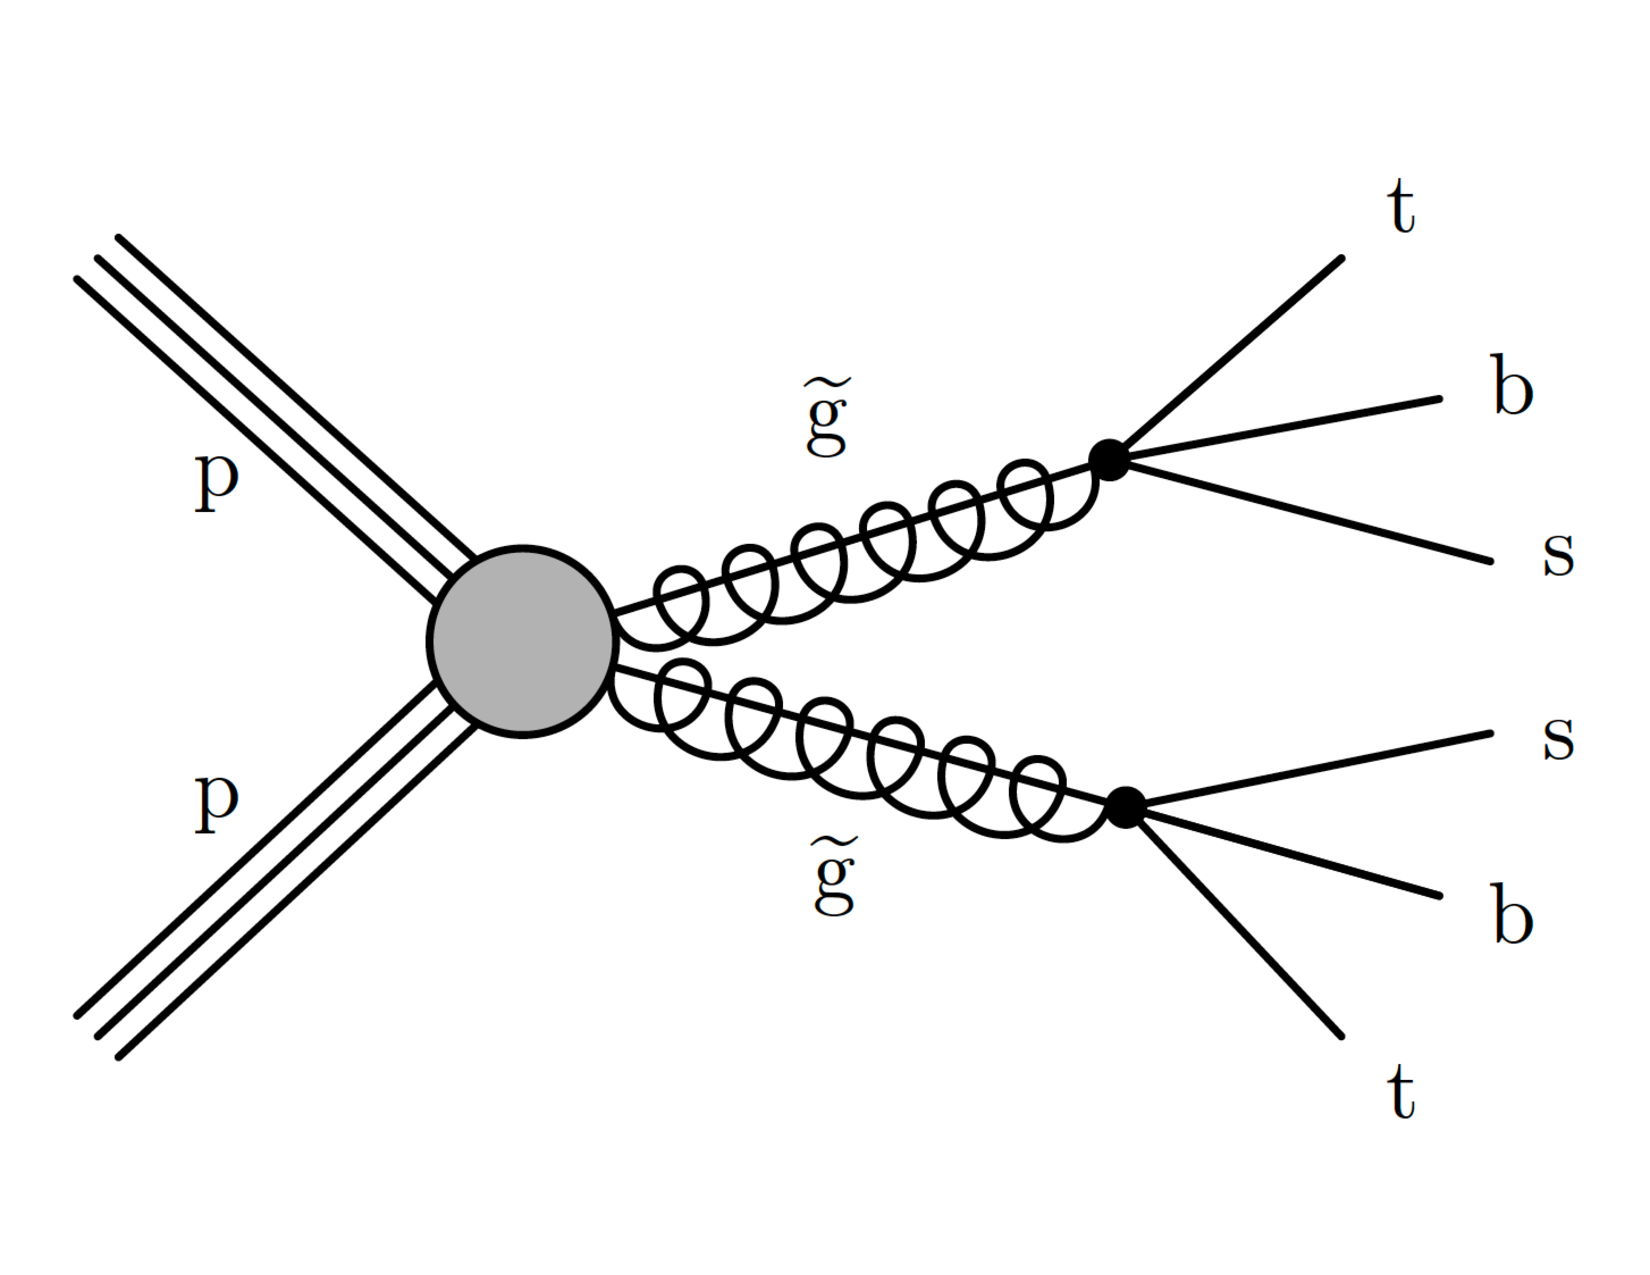
\includegraphics[width=0.45\textwidth]{figs/ssp/diag_T1tbs}} \\
\caption{Diagrams illustrating the two simplified RPV SUSY models considered in this analysis.}
\label{fig:susy_diag_set3}
\end{figure}

A summary of the 14 simplified SUSY models considered in the inclusive SUSY analysis
is shown in Table~\ref{tab:susyprocesses}. The last few columns give final state multiplicities
of bosons and \PQb quarks. At a glance, based on the high multiplicity of $\PW$ and $\PZ$ bosons,
it is clear that these models result in SS final states and many jets.

\begin{table} [h!]
\begin{center}
\resizebox{0.99\textwidth}{!}{
{\renewcommand{\arraystretch}{1.85}
\begin{tabular}{l|p{0.4\textwidth}cccccccc}
\hline
Model & Process & Constraint & Mass 1 & Mass 2 & RPV & \#W & \#Z & \#H & \#b\\
\hline
\Totttt & $\gluino\to\ttbar\lsp$ & \NA & $m_{\gluino}$ & $m_{\lsp}$ & \NA  & 4 & 0 & 0 & 4 \\
\TfttbbWW & $\gluino\to\cPqt\cPqb\chiplmin$ & $m_{\chiplmin}=m_{\lsp}+5\GeV$ & $m_{\gluino}$ & $m_{\lsp}$ & \NA & 4 & 0 & 0 & 4 \\
\Tftttt & $\gluino\to\susytopone\cPqt$, $\susytopone\to\cPqt\lsp$ & $m_{\susytop}-m_{\lsp}=m_{\PQt}$ & $m_{\gluino}$ & $m_{\lsp}$ & \NA  & 4 & 0 & 0 & 4 \\
\Tfttcc & $\gluino\to\susytopone\cPqt$, $\susytopone\to\cPqc\lsp$ & $m_{\susytop}-m_{\lsp}=20\GeV$&  $m_{\gluino}$ & $m_{\lsp}$ & \NA  & 2 & 0 & 0 & 2 \\
\TfqqqqWW & $\gluino\to\cPq\cPq'\chiplmin$, $\chiplmin\to\PW^{\pm}\lsp$ & $m_{\chiplmin}=0.5(m_{\gluino}+m_{\lsp})$ & $m_{\gluino}$ & $m_{\lsp}$ & \NA  & 2 & 0 & 0 & 0 \\
\TfqqqqWW & $\gluino\to\cPq\cPq'\chiplmin$, $\chiplmin\to\PW^{\pm}\lsp$ & $m_{\chiplmin}=m_{\lsp}+20\GeV$ & $m_{\gluino}$ & $m_{\lsp}$ & \NA  & 2 & 0 & 0 & 0 \\
\TfqqqqWZ & $\gluino\to\cPq\cPq'(\chiplmin/\neutralinotwo)$, \newline $\chiplmin\to\PW^{\pm}\lsp$, $\neutralinotwo\to\PZ\lsp$ & $m_{\chiplmin}=0.5(m_{\gluino}+m_{\lsp})$ & $m_{\gluino}$ & $m_{\lsp}$ & \NA  & 1 & 1 & 0 & 0 \\
\TfqqqqWZ & $\gluino\to\cPq\cPq'(\chiplmin/\neutralinotwo)$, \newline $\chiplmin\to\PW^{\pm}\lsp$, $\neutralinotwo\to\PZ\lsp$ & $m_{\chiplmin}=m_{\lsp}+20\GeV$ & $m_{\gluino}$ & $m_{\lsp}$ & \NA  & 1 & 1 & 0 & 0 \\
\TsttWW & $\sbottomone\to\cPqt\chiplmin$ & $m_{\lsp}=50\GeV$ & $m_{\sbottomone}$ & $m_{\chiplmin}$ & \NA  & 4 & 0 & 0 & 2 \\
\TsttHZ & $\susytoptwo\to\susytopone\PH$, $\susytopone\to\cPqt\lsp$ & $m_{\susytopone}-m_{\lsp}=175\GeV$ & $m_{\susytoptwo}$ & $m_{\susytopone}$ & \NA  & 0 & 0 & 2 & 2 \\
\TsttHZ & $\susytoptwo\to\susytopone(\PH/\PZ)$, $\susytopone\to\cPqt\lsp$ & $m_{\susytopone}-m_{\lsp}=175\GeV$&  $m_{\susytoptwo}$ & $m_{\susytopone}$ & \NA  & 0 & 1 & 2 & 4 \\
\TsttHZ & $\susytoptwo\to\susytopone\PZ$, $\susytopone\to\cPqt\lsp$ & $m_{\susytopone}-m_{\lsp}=175\GeV$ & $m_{\susytoptwo}$ & $m_{\susytopone}$ & \NA  & 0 & 2 & 0 & 2 \\
\ToqqqqL & $\gluino\to\cPq\cPq\bar{\cPq}\bar{\cPq}+e/\mu/\tau$ & \NA & $m_{\gluino}$ & \NA & Yes  & 0 & 0 & 0 & 0 \\
\Totbs & $\gluino\to\cPqt\cPqb\cPqs$ & \NA & $m_{\gluino}$ & \NA & Yes  & 2 & 0 & 0 & 4 \\
\hline
\end{tabular}}}
\caption{Summary of simplified SUSY models considered in this thesis. The fourth and
and fifth columns give the one or two masses which are scanned over for simplified interpretations.
The sixth column
marks processes with R parity violation. The remaining columns give the final state multiplicities
of $\PW$, $\PZ$, and Higgs bosons, and \PQb quarks, respectively.}
\label{tab:susyprocesses}
\end{center}
\end{table}

% \begin{table} [h!]
% \begin{center}
% \resizebox{0.99\textwidth}{!}{
% {\renewcommand{\arraystretch}{1.7}
% \begin{tabular}{l|p{0.4\textwidth}cccc}
% \hline
% Model & Process & Constraint & Mass 1 & Mass 2 & RPV? \\
% \hline
% \Totttt & $\gluino\to\ttbar\lsp$ & \NA & $m_{\gluino}$ & $m_{\lsp}$ & \NA \\
% \TfttbbWW & $\gluino\to\cPqt\cPqb\chiplmin$ & $m_{\chiplmin}=m_{\lsp}+5\GeV$ & $m_{\gluino}$ & $m_{\lsp}$ & \NA \\
% \Tftttt & $\gluino\to\susytopone\cPqt$, $\susytopone\to\cPqt\lsp$ & $m_{\susytop}-m_{\lsp}=m_{\PQt}$ & $m_{\gluino}$ & $m_{\lsp}$ & \NA \\
% \Tfttcc & $\gluino\to\susytopone\cPqt$, $\susytopone\to\cPqc\lsp$ & $m_{\susytop}-m_{\lsp}=20\GeV$&  $m_{\gluino}$ & $m_{\lsp}$ & \NA \\
% \TfqqqqWW & $\gluino\to\cPq\cPq'\chiplmin$, $\chiplmin\to\PW^{\pm}\lsp$ & $m_{\chiplmin}=0.5(m_{\gluino}+m_{\lsp})$ & $m_{\gluino}$ & $m_{\lsp}$ & \NA \\
% \TfqqqqWW & $\gluino\to\cPq\cPq'\chiplmin$, $\chiplmin\to\PW^{\pm}\lsp$ & $m_{\chiplmin}=m_{\lsp}+20\GeV$ & $m_{\gluino}$ & $m_{\lsp}$ & \NA \\
% \TfqqqqWZ & $\gluino\to\cPq\cPq'(\chiplmin/\neutralinotwo)$, \newline $\chiplmin\to\PW^{\pm}\lsp$, $\neutralinotwo\to\PZ\lsp$ & $m_{\chiplmin}=0.5(m_{\gluino}+m_{\lsp})$ & $m_{\gluino}$ & $m_{\lsp}$ & \NA \\
% \TfqqqqWZ & $\gluino\to\cPq\cPq'(\chiplmin/\neutralinotwo)$, \newline $\chiplmin\to\PW^{\pm}\lsp$, $\neutralinotwo\to\PZ\lsp$ & $m_{\chiplmin}=m_{\lsp}+20\GeV$ & $m_{\gluino}$ & $m_{\lsp}$ & \NA \\
% \TsttWW & $\sbottomone\to\cPqt\chiplmin$ & $m_{\lsp}=50\GeV$ & $m_{\sbottomone}$ & $m_{\chiplmin}$ & \NA \\
% \TsttHZ & $\susytoptwo\to\susytopone\PH$, $\susytopone\to\cPqt\lsp$ & $m_{\susytopone}-m_{\lsp}=175\GeV$ & $m_{\susytoptwo}$ & $m_{\susytopone}$ & \NA \\
% \TsttHZ & $\susytoptwo\to\susytopone(\PH/\PZ)$, $\susytopone\to\cPqt\lsp$ & $m_{\susytopone}-m_{\lsp}=175\GeV$&  $m_{\susytoptwo}$ & $m_{\susytopone}$ & \NA \\
% \TsttHZ & $\susytoptwo\to\susytopone\PZ$, $\susytopone\to\cPqt\lsp$ & $m_{\susytopone}-m_{\lsp}=175\GeV$ & $m_{\susytoptwo}$ & $m_{\susytopone}$ & \NA \\
% \ToqqqqL & $\gluino\to\cPq\cPq\bar{\cPq}\bar{\cPq}+e/\mu/\tau$ & \NA & $m_{\gluino}$ & \NA & Yes \\
% \Totbs & $\gluino\to\cPqt\cPqb\cPqs$ & \NA & $m_{\gluino}$ & \NA & Yes \\
% \hline
% \end{tabular}}}
% \caption{Summary of simplified SUSY models considered in this analysis. The third
% and second from last columns give the one/two masses which are scanned over. The last column
% marks processes with R parity violation.}
% \label{tab:susyprocesses}
% \end{center}
% \end{table}

\FloatBarrier

\section{Contributions to \tttt production}

SM \tttt production has a next-to-leading-order (NLO) cross section of 
$\xsectttt = 12.0^{+2.2}_{-2.5}~\unit{fb}$
at 13\TeV, calculated in Ref.~\cite{THEORY:Frederix2017wme},
with representative leading-order Feynman diagrams shown in
Fig.~\ref{fig:ftdiags}.
While it is interesting in its own right to measure a rare SM process,
searching for SM \tttt could provide hints of BSM physics.
Contributions from BSM physics to \tttt production at CMS can be 
broadly categorized as on-shell (usually involving heavy BSM intermediate particles coupling
to $\ttbar$), or off-shell (usually involving light BSM intermediate particles, or
modifications to the SM Higgs boson propagator or couplings).

\begin{figure}[!hbtp]
\centering
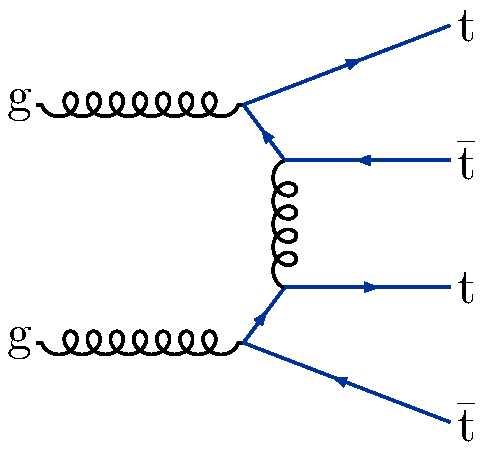
\includegraphics[width=0.35\textwidth]{figs/ftp/ftdiag1.pdf}
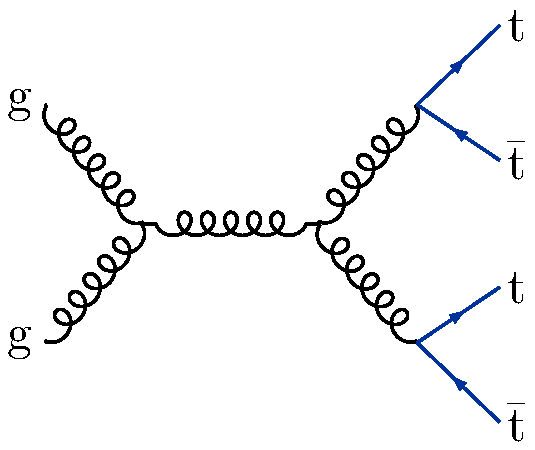
\includegraphics[width=0.35\textwidth]{figs/ftp/ftdiag2.pdf} \\
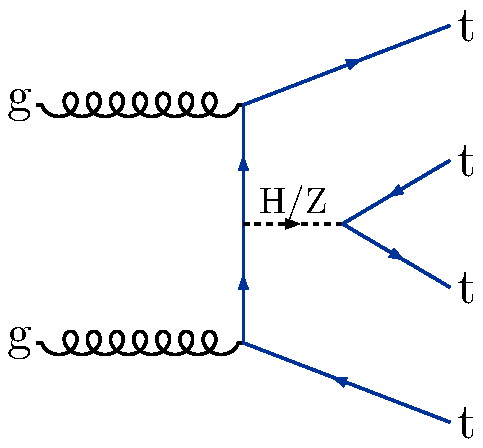
\includegraphics[width=0.35\textwidth]{figs/ftp/ftdiag4.pdf}
\caption{Typical Feynman diagrams for \tttt production at leasting order in the SM.}
\label{fig:ftdiags}
\end{figure}

\subsection{On-shell}

\subsubsection{Two Higgs doublet models}
\label{sec:ft2hdm}

In the spirit of generality, a simple possible extension of the SM 
is the two Higgs doublet model (2HDM)~\cite{THEORY:Branco2011iw}.
For example, the Minimal Supersymmetric Standard Model (MSSM)
has two Higgs doublets instead of the SM's single doublet.
Two doublets provides for five physical states: 
a light scalar boson $h$, a heavy scalar boson $\PH$, a heavy pseudoscalar boson $\PSA$, and
two charged bosons $\PH^\pm$. Their masses ($m_h, m_\PH, m_\PSA, m_{\PH^\pm}$)
constitute four of the six parameters used in the 2HDM. The other two are $\tan\beta$,
which is the ratio of vacuum expectation values of the two Higgs doublets,
and $\alpha$, which is the rotation angle that diagonalizes the mass matrix of the
two CP-even scalar states $h$ and $\PH$.

Given the observation of a new boson in 2012~\cite{CMS:HiggsObservation,ATLAS:HiggsObservation},
which has since been shown to have very SM Higgs-like properties,
there should be a phenomenological constraint on 2HDM theories to
account for this. Fortunately, in a Type-II 2HDM in the alignment limit,
$\sin(\beta-\alpha)\rightarrow 1$,
the CP-even scalar $h$ has
couplings which are SM-like, meaning it can be identified with the discovered particle,
and other states constitute new physics to be discovered.

In Type-II 2HDM, the couplings of the heavy scalar and pseudoscalar to SM
vector bosons are also suppressed, and vanish as
$\cos(\beta-\alpha)\rightarrow 0$. In this limit, production happens mainly
through gluon-fusion. However, the direct search for such new physics via
resonant \ttbar production is hampered by interference with the large SM
production of \ttbar~\cite{THEORY:Gaemers1984sj,THEORY:Dicus1994bm}. As an
alternative to direct production, since the branching ratio of the heavy
scalar state $\PH$ to up-type quarks (e.g., the top quark) is proportional to
$1/\tan\beta$, at low $\tan\beta$, associated production with three and four
top quark final states provide a relatively clean handle to probe Type-II
2HDM scenarios~\cite{THEORY:Craig2015jba,THEORY:Craig2016ygr}. The one or two top quark
associated production modes are shown in Fig.~\ref{fig:thdm_diagrams}, where
the intermediate heavy boson decays into $\ttbar$ at low $\tan\beta$, resulting in
final states of $\tttt$, $\PQt\bar{\PQt}\PQt\PW$, and $\PQt\bar{\PQt}\PQt\PQq$, respectively.
Heavy boson with masses above twice that of the top quark ($m_{\PH/\PSA}>350~\GeV$)
almost exclusively decay into \ttbar.
Thus, a SM search for \tttt would be optimized to directly probe the first of these three final states,
while still retaining sensitivity to the latter two, for sufficiently massive 
scalar and pseudoscalar bosons to allow for on-shell decays into \ttbar.

\begin{figure}[htbp!]
    \centering
    \subfloat[]{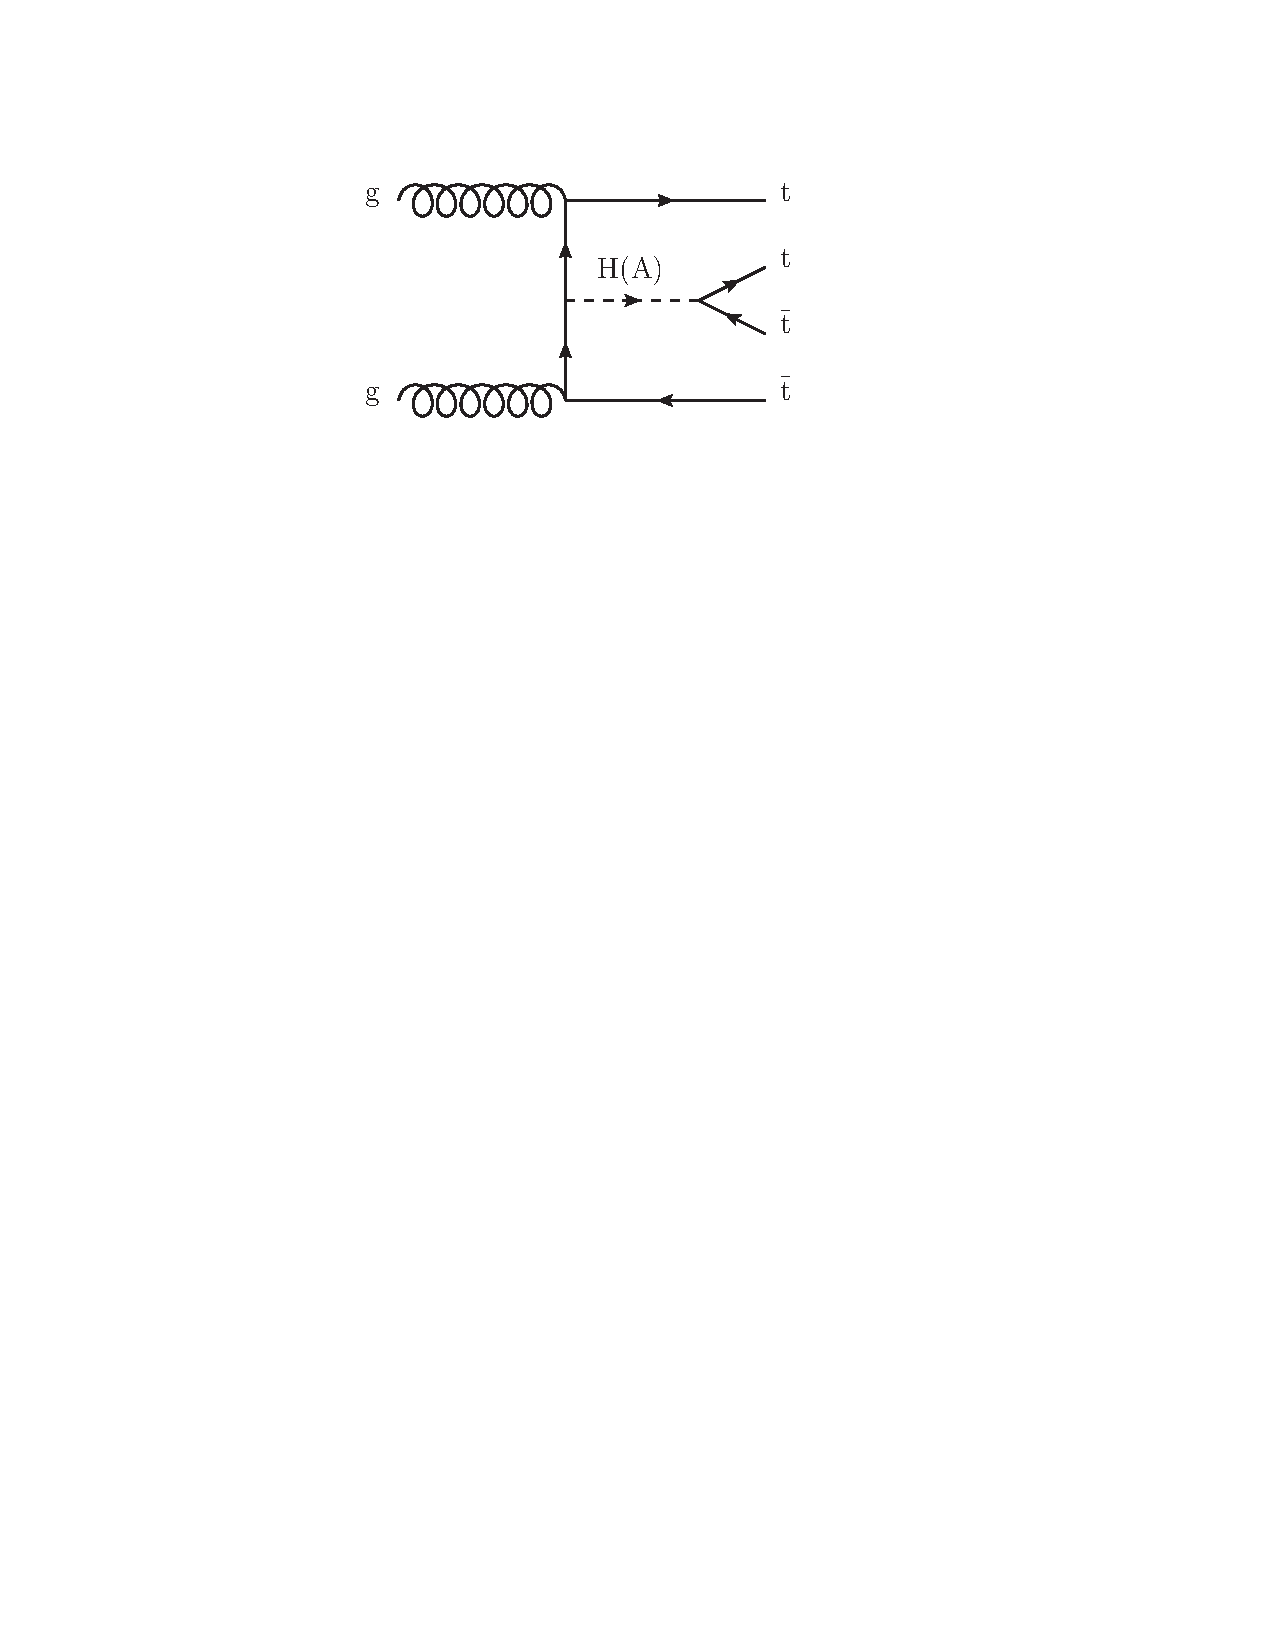
\includegraphics[width=0.44\textwidth]{figs/ftan/bsm_tth_diagram}}
    \subfloat[]{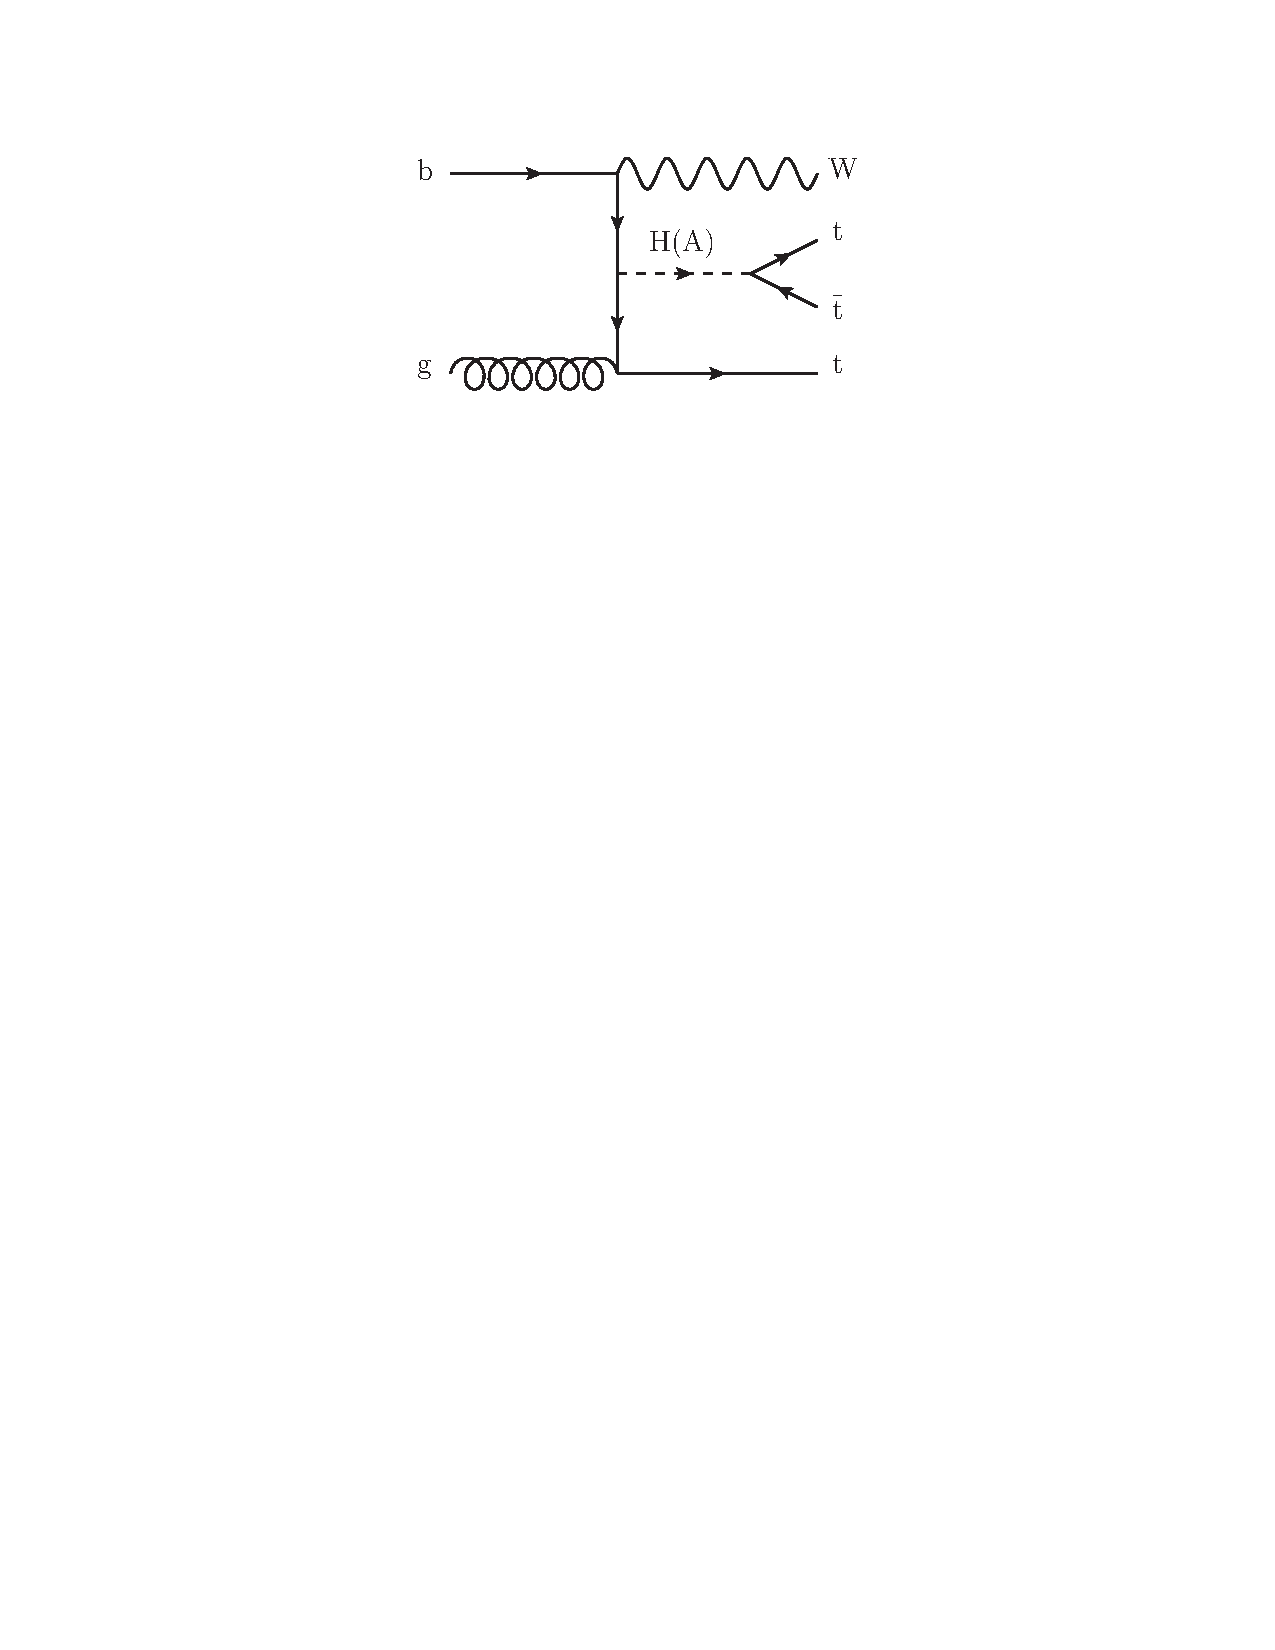
\includegraphics[width=0.44\textwidth]{figs/ftan/bsm_thw_diagram}} \\
    \subfloat[]{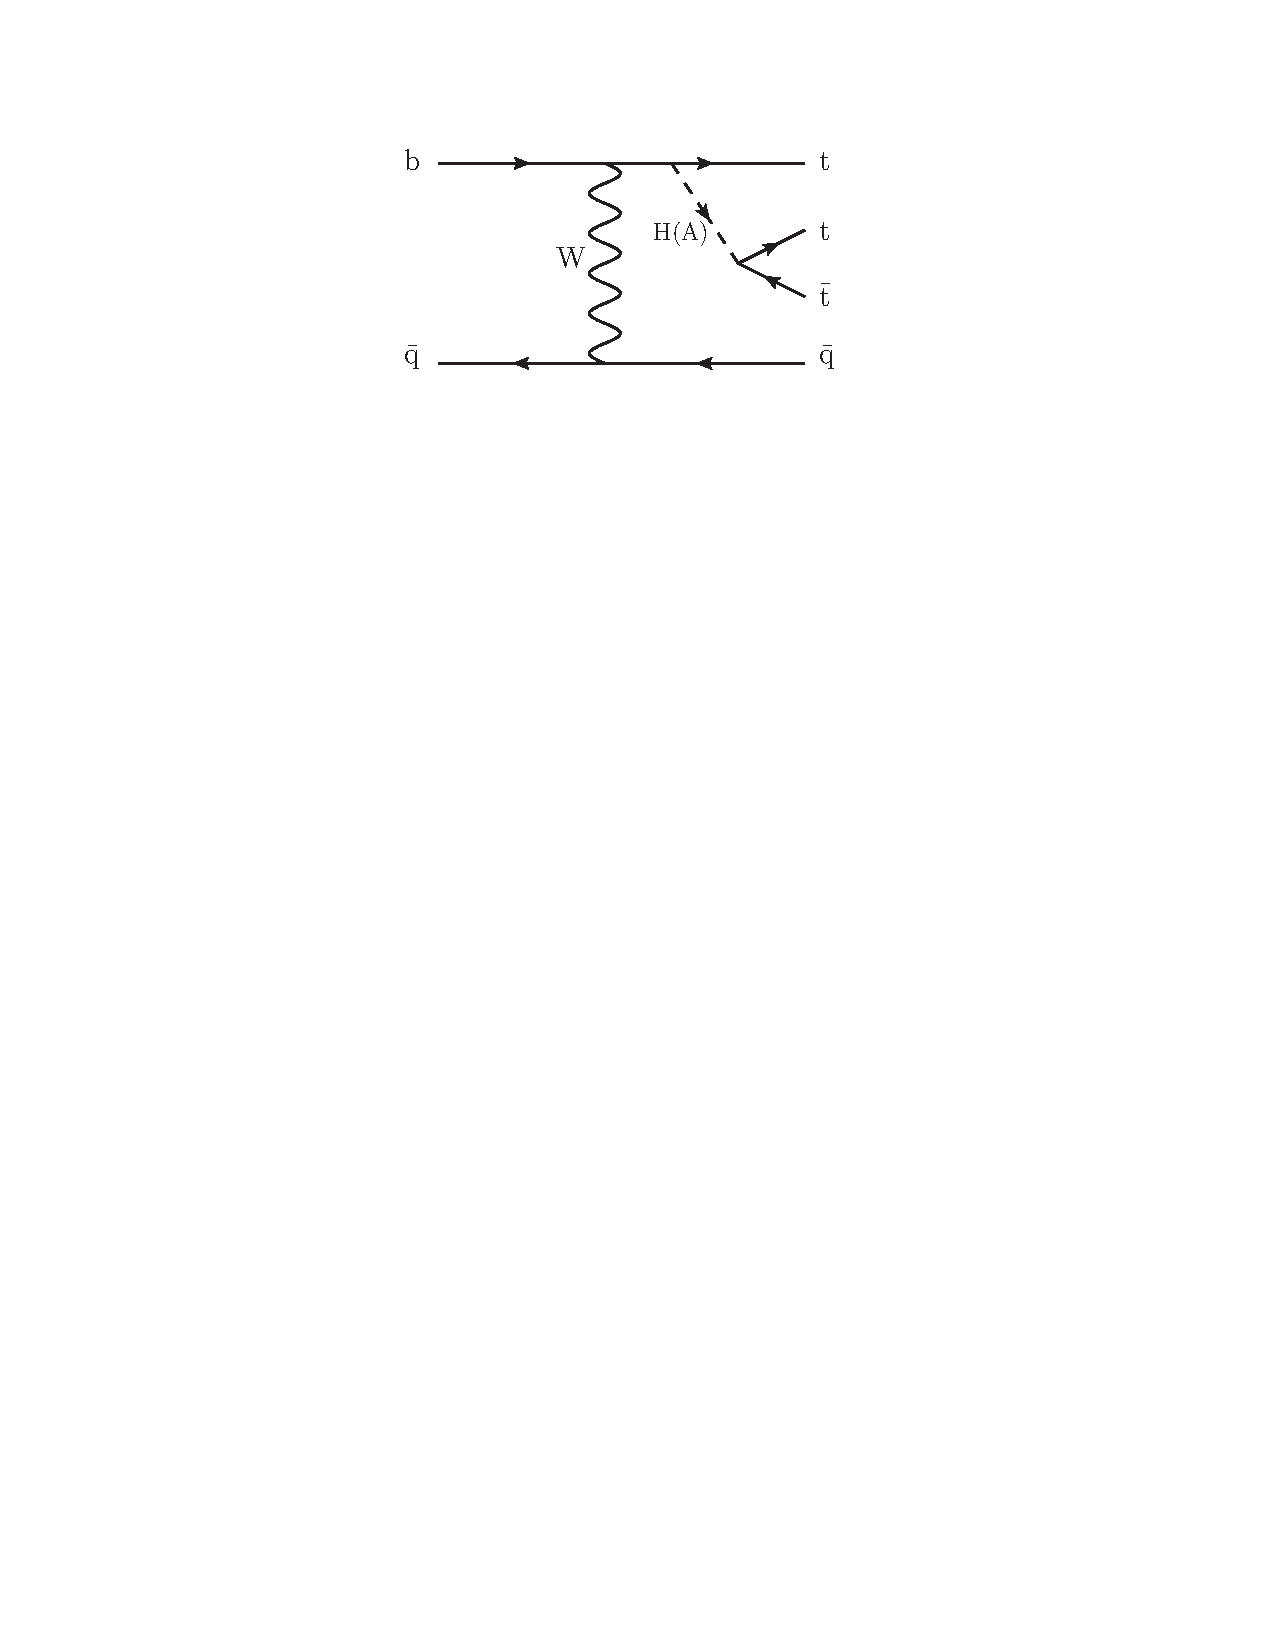
\includegraphics[width=0.44\textwidth]{figs/ftan/bsm_thq_diagram}}
\caption{Diagrams for scalar (pseudoscalar) production in association with 
one or two top quarks.}
\label{fig:thdm_diagrams}
\end{figure}

\FloatBarrier

Leading order cross sections (times branching ratio into \ttbar),
obtained similarly to Ref.~\cite{THEORY:Craig2016ygr},
for a
Type-II 2HDM scenario in the exact alignment limit are shown in
Fig.~\ref{fig:thdm_2d_xsecs}, as a function of mediator mass and $\tan\beta$.
Processes with $\PH$ and $\PSA$ mediators are considered separately and the
charged bosons $\PH^\pm$ are decoupled by setting their masses to 10\TeV.
Cross sections are generally slowly falling as a function of increasing mass
and sharply falling for increasing $\tan\beta$. One dimensional cross
section plots for three particular values of $\tan\beta$ are shown in
Fig.~\ref{fig:thdm_1d_xsec}, and range from approximately $45\unit{fb}$ at the
$2m_\PQt$ threshold to $9\unit{fb}$ at $m_\PH=650~\GeV$ for $\tan\beta=1$.

\begin{figure}[htb!]
    \centering
    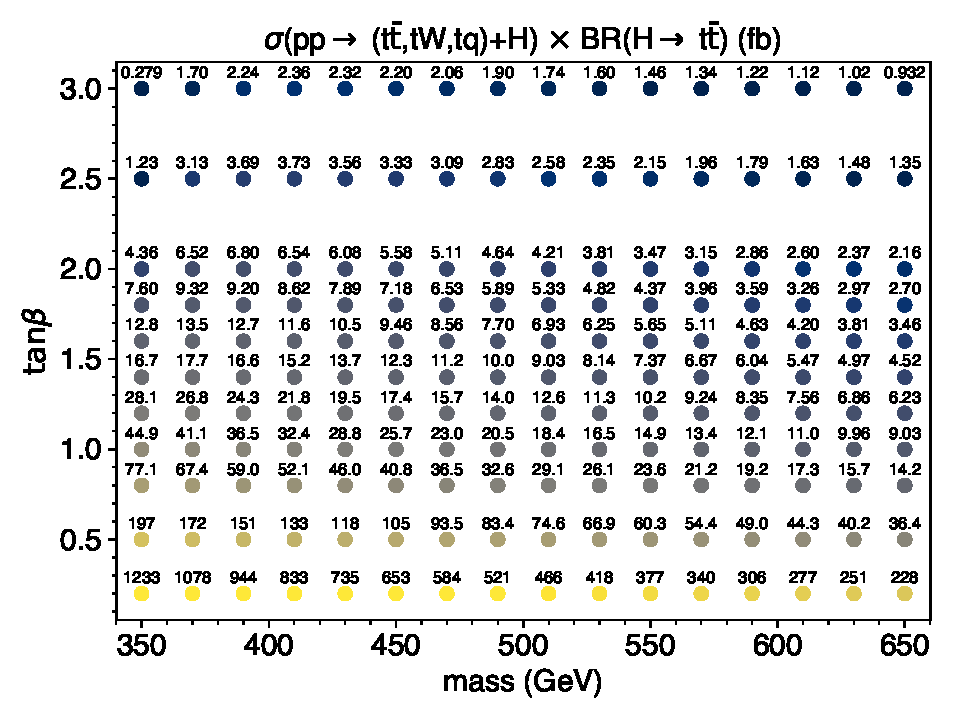
\includegraphics[width=0.75\textwidth]{figs/ftan/plot_2d_2hdm_xsec_h} \\
    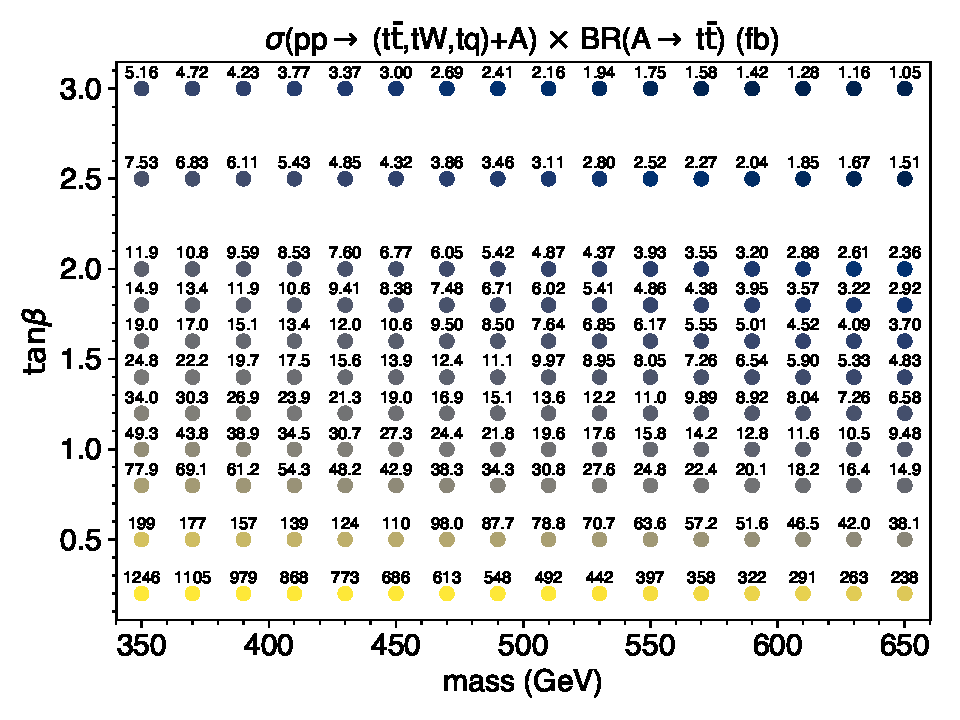
\includegraphics[width=0.75\textwidth]{figs/ftan/plot_2d_2hdm_xsec_a}
\caption{Cross sections times branching ratio into \ttbar for a heavy scalar boson $\PH$ (top) 
or heavy pseudocalar boson $\PSA$ (bottom) as a function of boson mass and $\tan\beta$.}
\label{fig:thdm_2d_xsecs}
\end{figure}

\begin{figure}[htb!]
    \centering
    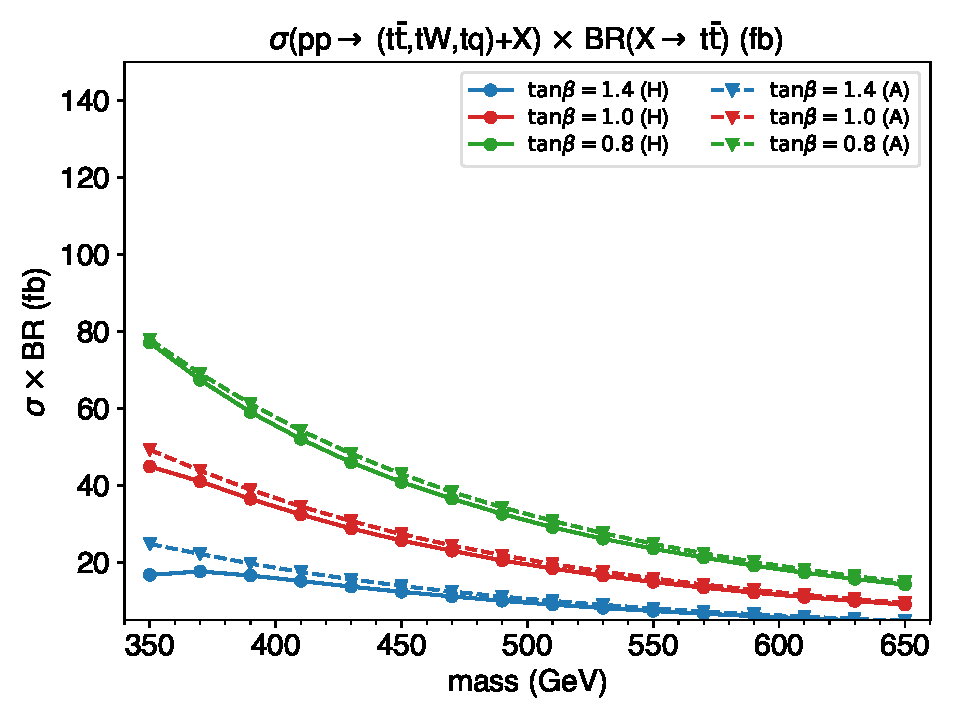
\includegraphics[width=0.75\textwidth]{figs/ftan/plot_1d_2hdm_xsec}
\caption{Cross sections times branching ratio into \ttbar for a heavy scalar boson $\PH$ 
or heavy pseudocalar boson $\PSA$ as a function of boson mass for three assumptions of 
$\tan\beta$ ($0.8, 1.0, 1.4$).}
\label{fig:thdm_1d_xsec}
\end{figure}

\FloatBarrier

\subsubsection{Simplified dark matter models}
\label{sec:ftdm}

Similarly to 2HDM, simplified dark matter (DM) models with scalar or pseudoscalar
mediators decaying into a pair of dark matter or SM particles can be
probed~\cite{THEORY:DMsingletop}. The production of these mediators,
and subsequent decay into invisible dark matter particles,
in association with a one or two top
quarks, was performed by CMS with the 2016 dataset
Ref.\cite{CMS:DMsingletop,CMS:DMttpair}. The production diagrams are shown in
Fig.~\ref{fig:dm_diagrams}.

In the framework of a simplified dark matter model, where the scalar ($\phi$)
or pseudoscalar ($\mathrm{a}$) mediator couples dark matter and SM particles,
the relevant terms of the interaction lagrangian are of the form
\[
    \mathcal{L}_{\phi}=g_{\chi}\phi\bar{\chi}\chi + \frac{g_\mathrm{q} \phi}{\sqrt{2}} \sum_{\mathrm{f}} y_\mathrm{f} \bar{\mathrm{f}} \mathrm{f}
    \quad\quad\quad
    \mathcal{L}_{a}=i g_{\chi}a\bar{\chi}\gamma^5\chi + \frac{i g_\mathrm{q} \mathrm{a}}{\sqrt{2}} \sum_{\mathrm{f}} y_\mathrm{f} \bar{\mathrm{f}} \gamma^5 \mathrm{f}
\]
where $y_\mathrm{f}$ are the fermionic yukawa couplings. The coupling
constants $g_\chi$ and $g_\mathrm{q}$ give the relative strengths of the
mediator coupling to dark matter and SM particles, and are used
interchangeably with $g_\mathrm{DM}$ and $g_\mathrm{SM}$, respectively. The
model has four free parameters ($g_\chi$, $g_\mathrm{q}$, $m_\chi$, and
$m_\mathrm{a}$) which are reduced to two with the assumption of $g_\chi =
g_\mathrm{q} = 1$.

When the mediator mass is above $2 m_\mathrm{t} \approx 350\GeV$, on-shell
decay to \ttbar becomes kinematically accessible, resulting in three or four top
quark final states, so we instead consider a version of the diagrams of
Fig.~\ref{fig:dm_diagrams} with a decay of the mediator into \ttbar rather
than a pair of (invisible) dark matter particles $\chi\bar{\chi}$.
Consequently, the production diagrams and kinematics are identical to those
of the Type-II 2HDM for certain assumptions of mediator mass, dark matter mass,
and $\tan\beta$, and $\phi/\mathrm{a}$ can be identified as $\PH/\PSA$.

In this way, the three or four top quark final states
allow complementarity with the CMS analysis from Ref.~\cite{CMS:DMsingletop} which relied on
a final state with \ttbar and missing transverse energy, provided that
the mediator mass is sufficiently large to allow for on-shell decays of the mediator into \ttbar.
Lower mediator masses are more effectively probed by Ref.~\cite{CMS:DMsingletop}.

The product of cross section and branching ratio of the mediators into \ttbar,
under the assumption of $g_\mathrm{DM}=g_\mathrm{SM}=1$,
calculated as in Ref.~\cite{CMS:DMsingletop}, is shown in 
Fig.~\ref{fig:dm_2d_xsecs}. Note that when $2 m_{\chi}>m_{\PH/\PSA}$,
the decay of the mediators into DM is suppressed in favor of the next-leading mode,
\ttbar, and thus the cross sections become independent of $m_\chi$ above the
marked diagonals. The cross sections at large $m_\chi$ are nearly
identical to those of the 2HDM with $\tan\beta = 1$ shown previously.
However, below the diagonal, the mediator prefers to decay into $\chi\bar{\chi}$
and a search for three or four top quark final states loses sensitivity.

\begin{figure}[htb!]
    \centering
    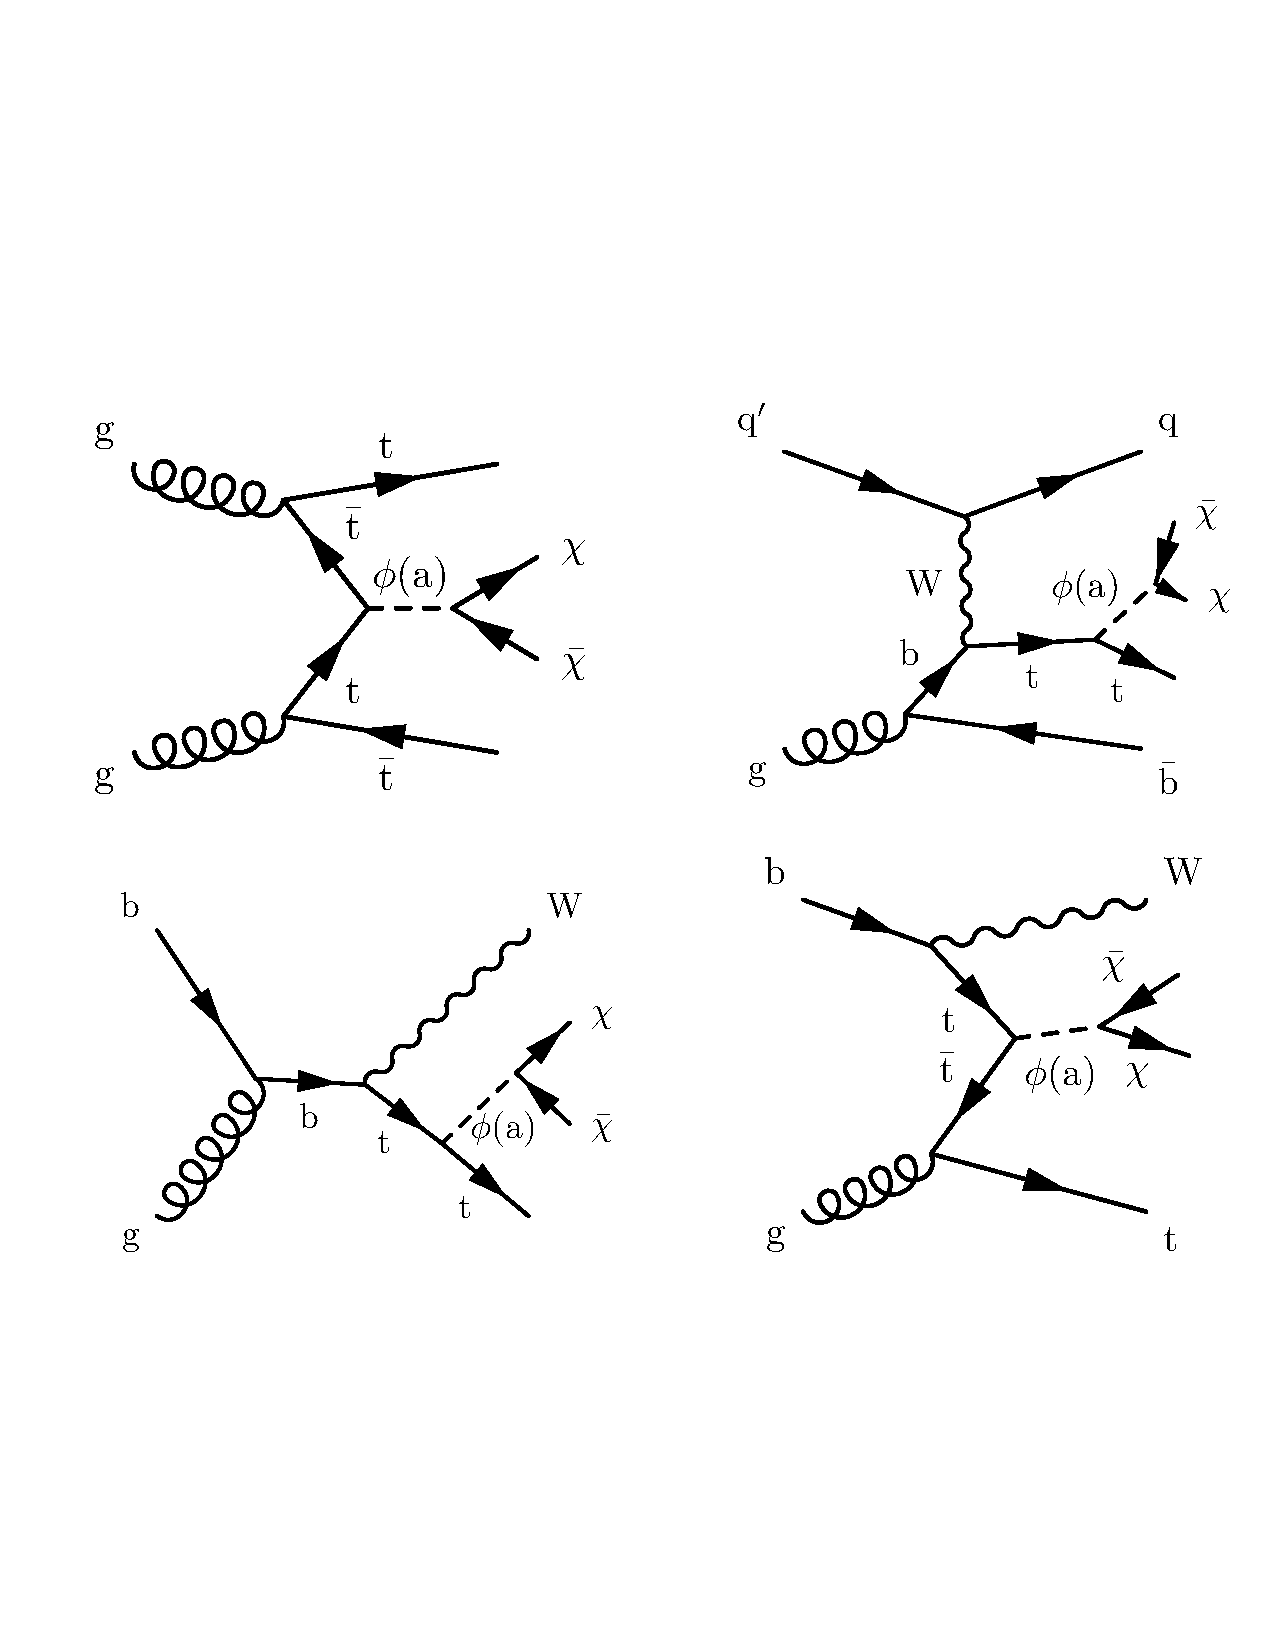
\includegraphics[width=0.75\textwidth]{figs/ftan/bsm_dm_diagrams}
\caption{Diagrams for scalar (pseudoscalar) production in association with a
\ttbar pair (top left), associated t-channel single top (top right),
associated $\PQt\PW$ (bottom row). The mediator subsequently decays into 
a pair of invisible DM particles $\chi\bar{\chi}$.}
\label{fig:dm_diagrams}
\end{figure}

\begin{figure}[htb!]
    \centering
    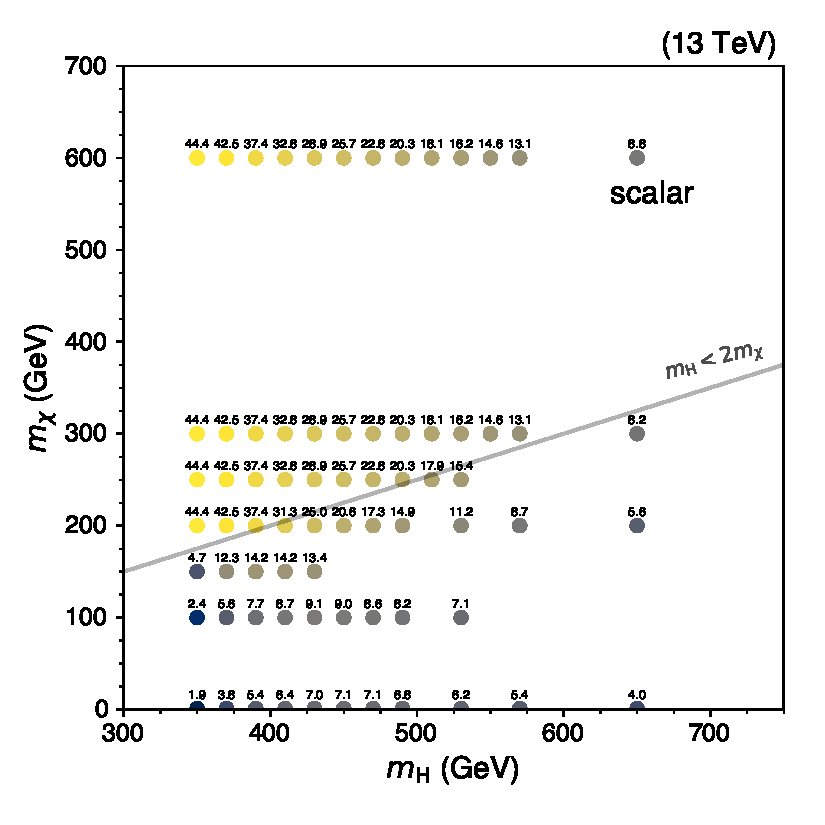
\includegraphics[width=0.60\textwidth]{figs/ftan/plot_2d_dmscalar_xsec_totsm} \\
    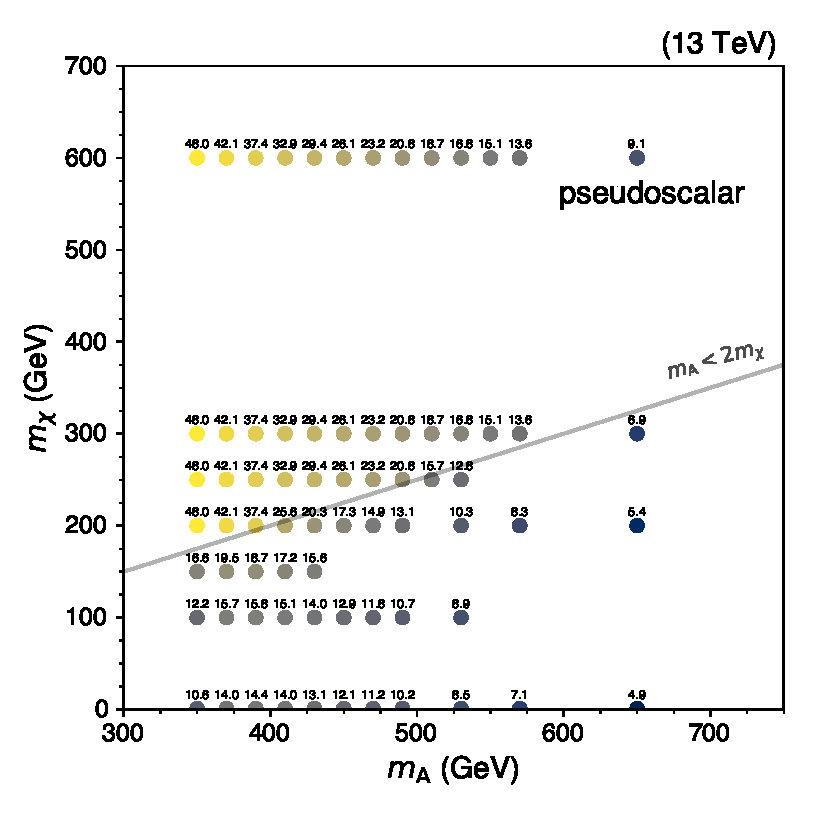
\includegraphics[width=0.60\textwidth]{figs/ftan/plot_2d_dmpseudo_xsec_totsm}
\caption{Cross sections (times branching ratio into $\ttbar$), in units of $\unit{fb}$, assuming
$g_\mathrm{DM}=g_\mathrm{SM}=1$, in the plane of $m_\chi$ versus $m_{\PH/\PSA}$ (top/bottom).
}
\label{fig:dm_2d_xsecs}
\end{figure}



\FloatBarrier

\subsection{Off-shell}

\subsubsection{Top quark yukawa coupling}
\label{sec:ftyukawa}

The SM $pp \rightarrow \tttt$ process includes diagrams with virtual Higgs bosons,
as shown in Fig.~\ref{fig:feynYukawa}. 
The amplitude corresponding to these diagrams is 
proportional to the square of the top Yukawa coupling,
and thus, the cross section of SM \tttt provides
a probe of the top quark Yukawa coupling.

\begin{figure}[!hbtp]
\centering
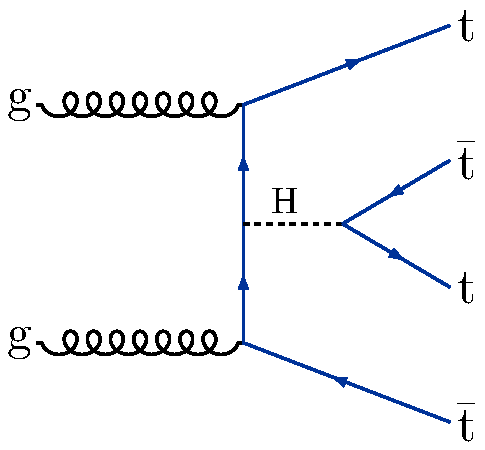
\includegraphics[width=.35\textwidth]{figs/ftp/ftdiag3.pdf} \\
\caption{One of the Feynman diagrams for \tttt including a virtual Higgs.}
\label{fig:feynYukawa}
\end{figure}

Using the notation of Reference~\cite{THEORY:TopYukawaTTTT} the \tttt cross section can be written 
as 

\begin{equation} 
\label{eq:yukawa}
\sigma(\tttt) = \sigma^{\text{SM}}(\tttt)_{g+Z/\gamma} + k_t^4 \sigma^{\text{SM}}(\tttt)_H + k_t^2 \sigma^{\text{SM}}_{\rm int}
\end{equation} 

\noindent where $k_t \equiv y_t/y_t^{\text{SM}}$, $y_t$ is the top Yukawa coupling, and $y_t^{\text{SM}}$ is its SM value.
In equation~\ref{eq:yukawa} the first term on the right hand side corresponds to the 
SM contribution to the cross section from diagrams with gluons or $Z/\gamma$, the second term
is the contribution from diagrams with virtual Higgs bosons, and the third term is the interference between
the two previous terms. Therefore, given a theoretical calculation and a measurement of $\sigma(\tttt)$, one can put 
constraints on $|y_t/y_t^{\text{SM}}|$.

The authors of Reference~\cite{THEORY:TopYukawaTTTT} have calculated the cross section terms at LO.
These are given in Table~\ref{tab:yukawa} and are shown in Fig.~\ref{fig:cross_section_yt},
where the figure shows a curve normalized such that the prediction matches the NLO calculation of 
the \tttt cross section of $12.0^{+2.2}_{-2.5}~\unit{fb}$.
The upper and lower values given in Table~\ref{tab:yukawa} correspond to variations
of the renormalization and factorization scale up and down by a factor of two, respectively.

\begin{table} [h!]
\begin{center}
{\renewcommand{\arraystretch}{1.3}
\begin{tabular}{l|ccc}
\hline
   & lower & central & upper \\
\hline
$ \sigma^{\text{SM}}(\tttt)_{g+Z/\gamma}  $ & 14.104 fb & 9.997 fb &  6.378 fb \\
$ \sigma^{\text{SM}}(\tttt)_H $                  & 1.625 fb &  1.167 fb &  0.7655 fb \\
$\sigma^{\text{SM}}_{\rm int} $                   & -2.152 fb &  -1.547 fb &  -0.999 fb \\
\hline
\end{tabular}}
\caption{LO calculation of the terms in equation~\ref{eq:yukawa} from
Reference~\cite{THEORY:TopYukawaTTTT}.  
The uncertainties are from private communications with the authors.}
\label{tab:yukawa}
\end{center}
\end{table}


\begin{figure}[!htbp]
    \centering
    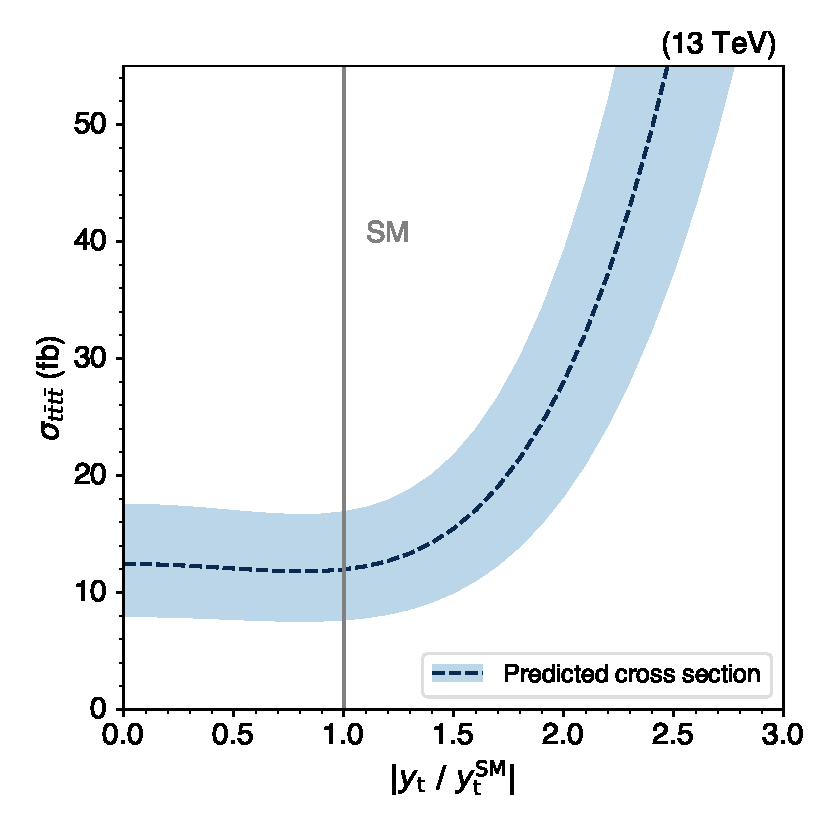
\includegraphics[width=0.75\linewidth]{figs/ftan/cross_section_yt.pdf}
    \caption{
        Predicted \tttt cross section as a function of $|y_t/y_t^{\text{SM}}|$.
    }
    \label{fig:cross_section_yt}
\end{figure}

\FloatBarrier

\subsubsection{Light off-shell mediators}
\label{sec:ftzprimephi}

The production of \tttt may also be influenced by a neutral scalar mediator
($\phi$) or neutral vector mediator ($Z'$) which couple to top quarks and have
masses less than twice the mass of the top quark, distinguishing them from
from similar processes within the 2HDM framework, for example. The off-shell contributions
to the SM \tttt production can be large, as shown in
Ref.~\cite{THEORY:Alvarez2016nrz}. For a large range of masses, kinematics are identical when considering these additional
processes, so that the total \tttt cross section is subject to a simple
rescaling.  Corresponding coupling terms in the lagrangian are of the form
\begin{equation}
    \mathcal{L}_{Z'}=-g_{t Z'}\bar{t}_R \slashed{Z}' t_R
    \quad\quad\quad
    \mathcal{L}_{\phi}=-g_{t \phi}\bar{t}_L \phi t_R
\end{equation}
There is an approximate independence of kinematics on the coupling strength and mediator mass~\cite{THEORY:Alvarez2016nrz},
so a single upper limit on the \tttt cross section can be used to place constraints 
on couplings $g_{tZ'}$ and $g_{t\phi}$ as a function of masses $m_{Z'}$ and $m_{\phi}$,
respectively.
Cross sections of \tttt (normalized to SM, and calculated as in Ref.~\cite{THEORY:Alvarez2016nrz}) as a function of $g_{tZ'}$ 
and $g_{t\phi}$, for different assumptions of $m_{Z'}$ and $m_{\phi}$,
are shown in Fig.~\ref{fig:cross_section_zprimephi}. To illustrate a particular example,
the horizontal dotted line in the figures represents excluding cross sections more than
double that of the SM. These are translated into exclusions on $g_{tZ'}$ and $g_{t\phi}$
via crossing points that are projected onto the x axis.

\begin{figure}[!htbp]
    \centering
    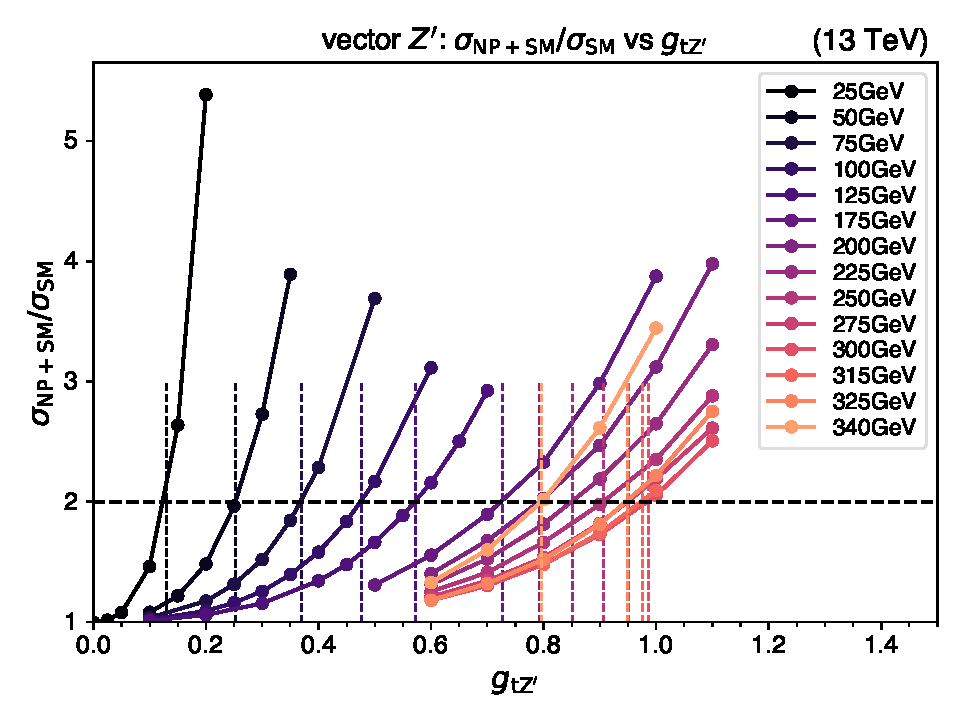
\includegraphics[width=0.78\linewidth]{figs/ftan/plot_xsec_zprime.pdf} \\
    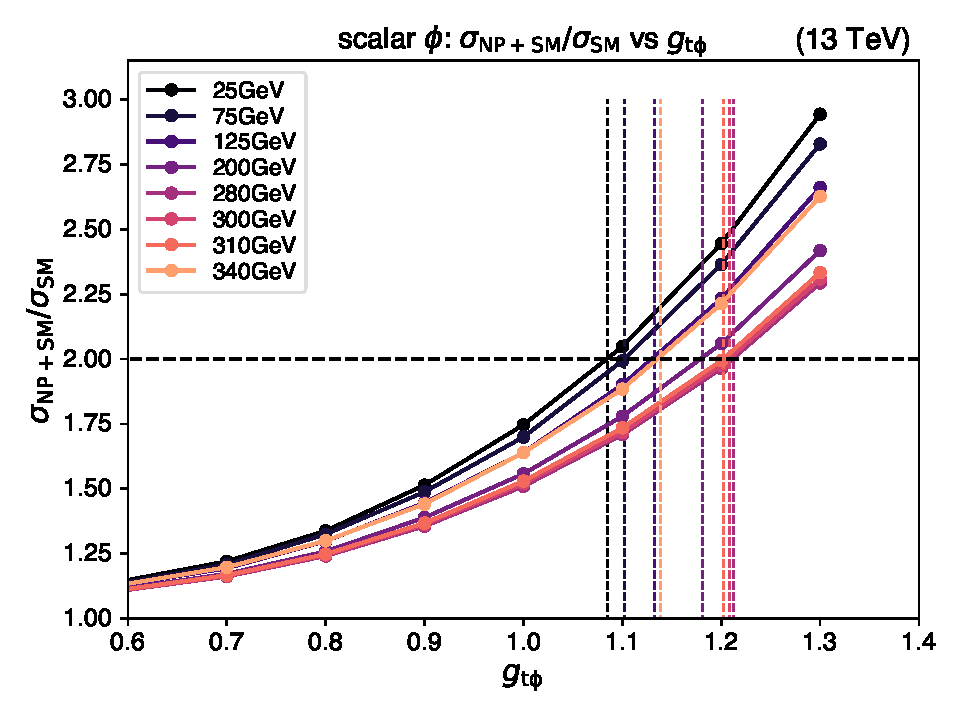
\includegraphics[width=0.78\linewidth]{figs/ftan/plot_xsec_phi.pdf}
    \caption{
        Cross sections of \tttt (normalized to SM) as a function of $g_{tZ'}$ (upper)
        and $g_{t\phi}$ (lower) for different assumptions of $m_{Z'}$ and $m_{\phi}$,
        respectively.
    }
    \label{fig:cross_section_zprimephi}
\end{figure}

\FloatBarrier

\subsubsection{Oblique Higgs parameter}
\label{sec:fthhat}

In a universal effective field theory framework, the Higgs oblique
parameter $\hat H$, defined as the Wilson coefficient of the dimension-6
operator modifying the Higgs boson propagator, can result in deviations of the
SM \tttt cross section, as shown in Ref.~\cite{THEORY:ObliqueHiggs2019}.  These
(off-shell) deviations can be constrained to a level which is competitive with
constraints from on-shell processes.

The two main characteristic effects of this oblique parameter are
an additional term in the SM Higgs boson propagator
\begin{equation}
    P_h(p^2)\approx\frac{i}{p^2-m_h^2}-\frac{i\hat{H}}{m_h^2},
\end{equation}
and a rescaling of the fermionic higgs
couplings
\begin{equation}
    \kappa_f = 1-{\hat H}.
\end{equation}

Using the latest combined fits from the ATLAS experiment for the (on-shell) fermionic couplings,
with 80$\mathrm{fb}^{-1}$ of 13\TeV data, Ref.~\cite{THEORY:ObliqueHiggs2019} finds a constraint on
the oblique parameter of $\hat{H} < 0.16$ at 95\% CL.

Ref.~\cite{THEORY:ObliqueHiggs2019} also calculates that the cross section of (off-shell) \tttt is subject to a fractional modification (with respect to the SM cross section)
at 14\TeV, given by,
\begin{equation}
    \frac{\sigma_{\hat{H}+\mathrm{SM}}}{\sigma_\mathrm{SM}} = 1 + 0.03\left(\frac{\hat{H}}{0.04}\right) + 0.15\left(\frac{\hat{H}}{0.04}\right)^2.
\end{equation}
For an oblique parameter value of 0.1, the formula predicts a doubling of the SM cross section of \tttt.

The SM model within the MadGraph~\cite{THEORY:MADGRAPH5} generator was modified to take into account the extra term in the propagator, as
well as the rescaling of the top-yukawa coupling, and the calculation is repeated
at 13\TeV. The resulting curve is shown in Fig.~\ref{fig:higgs_oblique_madgraph}.

When searching for SM \tttt and placing upper limits on the production cross
section, one can use the relative size of the upper limit with respect to
the SM prediction to exclude $\hat{H}$ values above a threshold. For example,
excluding cross sections more than double that of the SM, $\hat{H}$ values
above approximately 0.14 can be excluded. There are two important caveats
that will need to be taken into account when performing an interpretation for
$\hat{H}$. First, the kinematics of $\tttt$ will be slightly different
depending on the value of $\hat{H}$. Second, the SM process $\ttH$, which is
relevant for the $\tttt$ search, is proportional to
$y_\mathrm{t}^2=(1-\hat{H})^2$ ($\approx 0.74$ at $\hat{H}=0.14$).

\begin{figure}[!htbp]
    \centering
    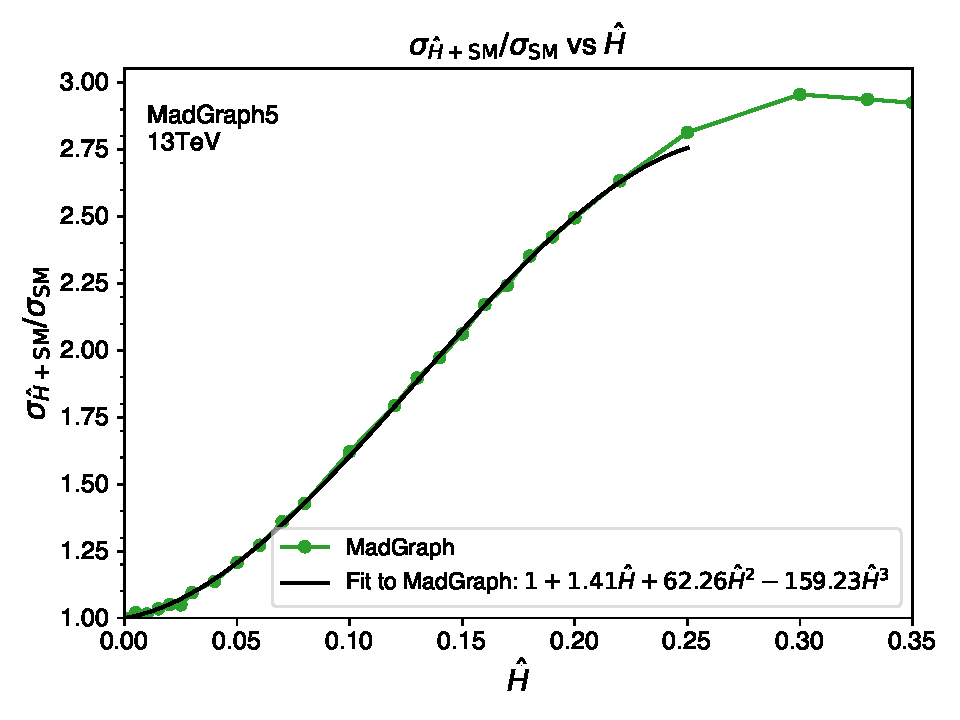
\includegraphics[width=0.75\linewidth]{figs/ftan/higgs_oblique.pdf}
    \caption{
        Cross section (normalized to SM) as a function of oblique parameter $\hat{H}$.
        The green curve is a calculation from MadGraph at 13\TeV, and
        the solid black curve is a cubic fit to the calculation.
    }
    \label{fig:higgs_oblique_madgraph}
\end{figure} % Same-sign dilepton final state
\chapter{Objects and selections}

\section{Jets, MET}

\subsection{Jets}
Jets are reconstructed from charged PF candidates clustered with the
anti-$\mathrm{k_t}$ algorithm~\cite{CMS:Cacciari2008gp, CMS:Cacciari2011ma}
using a distance parameter of 0.4. The jet \pt, calculated as the vector sum
of the constituent PF candidates, is susceptible to contributions from pileup
and detector effects. However, jet energy corrections, primarily
parameterized by jet \pt and $\eta$, are derived using data and simulation to
counteract these effects~\cite{CMS:Khachatryan2016kdb, CMS:PASJME16003}.

Additional jet selections (tight jet identification) are applied to reject
pathological jets:
\begin{itemize}
    \item neutral hadronic energy fraction $<$ 0.9
    \item neutral electromagnetic energy fraction $<$ 0.9
    \item number of constituents $>$ 1
    \item charged hadron fraction $>$ 0
    \item charged multiplicity $>$ 0
\end{itemize}

To avoid double counting of objects,
selected jets are those that do not overlap with analysis leptons 
(within a cone of $\Delta R \equiv \sqrt{\Delta\eta^2 + \Delta\phi^2} = 0.4$),
and have $\pt>40\GeV$ and $|\eta|<2.4$. The multiplicity of selected jets
is defined to be \Njets. The scalar sum of selected jet \pt
is called \HT.

\subsection{B-tagging}
Many of the SUSY models probed in this analysis have a high multiplicity of
top quarks; SM four top quark production has four. Each top quark decays into
a b quark and W boson, so jets arising from b quarks are an important object
to efficiently identify. Hadrons containing b quarks have lifetimes that
allow them to travel on the order of a millimeter from the collision before
decaying, creating tracks pointing to a secondary vertex. We use a deep
neural network algorithm, DeepCSV~\cite{CMS:Sirunyan2017ezt}, which makes use
of information such as tracks and secondary vertices to produce a
discriminating value for b jets. A threshold value (the medium working point)
on this discriminant is set such that the efficiency to correctly identify a
b jet is approximately 65\% for jet \pt around 40\GeV while maintaining a
misidentification rate of 1\% for light-flavor jets (udsg).
While they are not directly used here, there are two additional working points
for the b-tagging, loose and tight, which have 10\% and 0.1\% misidentification 
rates for light-flavor jets, respectively.

This \Nbjets variable is defined as the multiplicity 
of b-tagged jets with $\pt>25\GeV$ and $|\eta|<2.4$ which are
not overlapping with leptons. The lower threshold compared
to nominal jets above allows for increased signal acceptance for softer event
topologies.

\subsection{MET}

The missing transverse energy,
equivalently referred to as MET, $\slashed{E}_\mathrm{T}$, or $\ptmiss$, is defined
as the magnitude of the negative of the vectorial sum of the $\vec{p_\mathrm{T}}$ of PF candidates in an
event~\cite{CMS:Sirunyan2019kia}.

The MET has a Type-I correction applied, which fully propagates
the jet energy corrections into the computation:

\begin{equation}
    \vec{\slashed{E}}_\mathrm{T}
    = \vec{\slashed{E}}_\mathrm{T}^\mathrm{raw}
    - \sum_{\mathrm{jets}} \left( 
        \vec{p}_\mathrm{T,jet}^\text{corr} 
        - \vec{p}_\mathrm{T,jet}
    \right)
\end{equation}

Additional event-level filters detailed in \cite{CMS:JetMETFilters} are applied 
to reject pathological events associated with misreconstruction, or sources of 
detector noise.

\section{Leptons}

\subsection{Identification}

Muons are reconstructed by combining information from tracker hits
with those in the muon system to form a global fit.
The base identification criteria for reconstructed muons is encapsulated in the 
``medium muon ID''~\cite{CMS:Sirunyan2019yvv} and requires
a certain level of quality in the tracker and muon system track matching.

Analysis muons must have $\pt>10\GeV$ and $|\eta|<2.4$. 
We require that muons have a relative 
uncertainty less than 20\% on the reconstructed momentum ($\delta \pt/\pt<0.2$).
This ensures the charge of the momentum has not been misreconstructed.

Analysis electrons must have $\pt>15\GeV$ and $|\eta|<2.5$.
Electrons are identified by constructing a boosted decision tree (BDT) with
a variety of variables tied to the track
and ECAL deposits used to reconstruct the electron~\cite{CMS:Khachatryan2015hwa}.
These include 
\begin{itemize}
    \item ECAL shower-shape variables
    \begin{itemize}
    \item $\sigma_{i\eta i\eta}$ (weighted width of shower along $\eta$)
    \item $\sigma_{i\phi i\phi}$ (weighted width of shower along $\phi$)
    \item cluster circularity
    \item cluster $\eta$, $\phi$ widths
    \item $\mathrm{R_9}$, the ratio of energy in 3x3 to 5x5 set of towers surrounding the seed crystal
    \item H/E, the ratio of (adjacent) HCAL energy to ECAL deposits
    \end{itemize}
    \item track-cluster matching variables
    \begin{itemize}
    \item $E/p_\mathrm{in}$, $E/p_\mathrm{out}$, where $p_\mathrm{in/out}$ is the innermost/outermost track momentum
    \item $\Delta \eta_\mathrm{in}$ ($\eta$ difference between cluster and inner track)
    \item $\Delta \eta_\mathrm{out}$
    \item $\Delta \phi_\mathrm{in}$ ($\phi$ difference between cluster and inner track)
    \item $|1/E_\mathrm{clust} - 1/p|$
    \end{itemize}
    \item track variables
    \begin{itemize}
    \item $\chi^2$ quality of combinatorial track finder (CTF) and Gaussian-sum filter (GSF) tracks
    \item number of CTF and GSF hits
    \item $(p_\mathrm{in}-p_\mathrm{out})/p_\mathrm{in}$, fraction of energy lost through Brehmsstrahlung
    \end{itemize}
\end{itemize}

The BDT discriminant is converted into a boolean decision per lepton with
working points depending on the year and $\pt$, which will not be shown here 
for the sake of brevity. We simply take and refer to two boolean decisions
as the ``loose'' and ``tight" working points, where the tight WP has
relatively lower efficiency to select electrons,
but also a lower efficiency to misidentify
other objects as electrons.

For electrons, we additionally consider a conversion veto that locates and rejects $\gamma \rightarrow e^{+} e^{-}$,
and a ``number of expected missing inner hits'' variable, which is the number of 
detector hits in the inner tracker which should have registered a hit but did not.
Electrons must have no such missing hits.
Electrons must also have agreement between three different methods used to compute the charge~\cite{CMS:AN14164}.

For both electrons and muons, we require $|d_\mathrm{xy}| < 0.05\unit{cm}$,
$|d_\mathrm{z}| < 0.1\unit{cm}$,
$\mathrm{SIP}_\mathrm{3D} < 4$. The variables $|d_\mathrm{xy}|$ and $|d_\mathrm{z}|$ are the transverse and longitudinal
displacements between the primary interaction vertex (PV) and the point of closest approach (PCA) of the lepton's 
track, respectively. The 3D impact parameter significance, $\mathrm{SIP}_\mathrm{3D}$,
is defined as the 3D displacement between the PCA and PV divided by the measurement uncertainty.
The reconstructed vertex with the largest value of $\Sigma \pt^2$ is taken as
the PV. These variables and selections make sure the leptons are produced in a prompt fashion.

The final lepton reconstruction and identification efficiency is between
45\% and 70\% for electrons with $\pt > 25\GeV$, and between 70\% and 90\%
for muons in the same momentum range. In the lower momentum range of 15-25\GeV
for electrons, the efficiency is 40\%, and in the range of 10-25\GeV for muons,
the efficiency is 55\%. 

\subsection{Isolation}

Conceptually, a lepton can be labeled isolated if the ratio of 
energy in a cone surrounding the lepton to the energy of the lepton itself
(``relative isolation'') is below a certain threshold.
However, we instead use three more sophisticated variables, improving upon this concept for robustness,
to classify leptons as isolated:
\begin{itemize}
    \item ``mini-isolation'' $\miniiso$: 
    \begin{equation}
        \miniiso = \frac{\sum_R \pt(h^\pm) - \mbox{max}(0, \sum_R \pt(h^0)+\pt(\gamma) - \rho\mathcal{A}\left(\frac{R}{0.3}\right)^2}{\pt(\ell)}.
    \end{equation}
    where $\rho$ is the event-level energy density from pileup,
    and $\sum_R\pt(h^\pm)$, $\sum_R\pt(h^0)$, $\sum_R\pt(\gamma)$ 
    are the sums of the $\pt$ of charged hadrons, neutral hadrons, and photons, respectively.
    The sum is performed within a cone of radius $R$, which depends on lepton \pt:
    \begin{equation}
        R = \frac{10}{\mbox{min}(\mbox{max}(\pt(\ell), 50), 200)}
    \end{equation}
    The effective areas $\mathcal{A}$ are constants calculated in coarse bins of
    lepton $\eta$ such that the last term of the numerator represents the
    contribution from pileup and is subtracted off.
    Requiring $\miniiso$ to be below a particular value ensures that the
    lepton is isolated.

    \item \ptratio, defined as the ratio of the lepton \pt to the
    \pt of the jet geometrically closest to, or containing, the lepton:
    \begin{equation}
        \ptratio = \frac{\pt(\ell)}{\pt(\text{jet})}
    \end{equation}
    In order to avoid an
    over-correction on prompt leptons, the application of the jet energy
    correction to mitigate is only applied on the hadronic part of the jet.
    That is, the denominator of $\ptratio$ is corrected for pileup effects
    after the lepton is subtracted out, and the lepton is subsequently added back.

    \item \ptrel:
    \begin{equation}
        \ptrel=\frac{\left|\left(\vec{p}(\text{jet})-\vec{p}(\ell)\right) 
        \times \vec{p}(\ell)\right| }{|\vec{p}(\text{jet})-\vec{p}(\ell)|}
    \end{equation}
    This variable is a measure of the relative transverse separation between the lepton 
    and matching jet. For leptons arising from the decay of B mesons, for example,
    this quantity exhibits a kinematic cutoff of a few GeV. For leptons that
    happen to overlap accidentally with jets, \ptrel compares too uncorrelated
    quantities and exhibits no kinematic cutoff, so this quantity can be large.
    This property allows us to recover leptons that would be labeled non-isolated
    by the previous two variables.
\end{itemize}

Using the above three variables, we classify a lepton
as isolated if the following boolean condition is satisfied:
\begin{equation}
  \miniiso < I_1 \wedge ( \ptratio > I_2 \vee \ptrel > I_3 )
\end{equation}
where $I_i$ threshold values depend on the lepton flavor and PU conditions
of the flavor of the lepton. These values are tabulated in Table~\ref{tab:isoWPs}.

\begin{table}[h]
    \label{tab:isoWPs}
    \centering
    \caption{Isolation working points }
    \begin{tabular}{|l||c|c|c|c|}
        \hline
        & e/$\mu$ loose WP &  $\mu$ tight WP & e tight WP \\ \hline 
        $I_1$ & 0.4 & 0.16 (2016), 0.11 (2017/2018) & 0.12 (2016), 0.07 (2017/2018) \\
        $I_2$ & 0  & 0.76 (2016), 0.74 (2017/2018) & 0.80 (2016), 0.78 (2017/2018) \\
        $I_3$ & 0  & 7.2 (2016), 6.8 (2017/2018) & 7.2 (2016), 8.0 (2017/2018) \\ \hline
    \end{tabular}
\end{table}

\section{Other variables}

We make use of the minimum transverse mass ($\mtmin$) which is defined as:
\begin{equation}
    \mtmin = \mathrm{min}\left[ \mT(\ell_1, \ETm), \mT(\ell_2, \ETm)\right ]
\end{equation}
where a single transverse mass term is given by
\begin{equation}
    \mtmin = \sqrt{2\pt(\ell) \ETm (1-\cos\Delta \phi_{\ell,\ETm})}
\end{equation}
and $\Delta \phi_{\ell,\ETm}$ is the azimuthal separation between the lepton
and the \ptmiss vector.

For events where \ptmiss arises primarily from neutrinos from W boson decays,
as is the case with the pervasive $\ttbar$ and $W$ processes, this variable
has a kinematic cutoff at the W boson mass, $m_{W}$. Signal events
where the \ptmiss is generated from an energetic $\lsp$ particle
will not exhibit such a kinematic cutoff.

Figure~\ref{fig:mtminttbar} shows the distribution of $\mtmin$ for a signal hypothesis \Totttt and the
\ttbar background, with the W boson mass marked as a vertical line. It is clear that 
the \ttbar background is almost completely bounded by the W mass, while the signal has a
large tail extending beyond the W mass.

\begin{figure}[!hbtp]
\centering
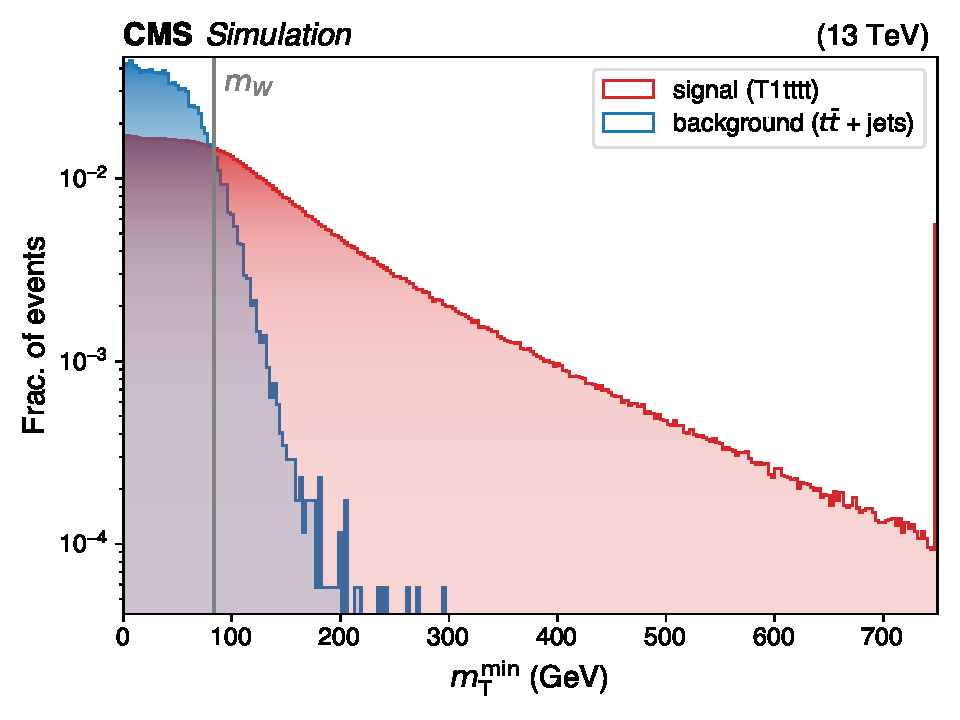
\includegraphics[width=.60\textwidth]{figs/misc/mtmin_signal_ttbar.pdf}
\caption{
    Normalized distribution of $\mtmin$ shown for signal hypothesis \Totttt and 
    \ttbar background.
}
\label{fig:mtminttbar}
\end{figure}

\section{Trigger}
\mytodo{todo, trigger plot}

Clearly before one can analyze events, one must have collected them with the detector first.
Triggers are meant to identify and save interesting events in data while making sure to not to overwhelm
the readout hardware, reconstruction software, and storage used by CMS. 
Same-sign searches make use of dilepton triggers
which require at least two leptons at trigger level of a given $\pt$, usually along with some
isolation quantities or $\HT$. For a given trigger rate, 
the more stringent the requirements on isolation or $\HT$, the
lower the thresholds on lepton $\pt$.

In the SUSY analysis, based on trigger thresholds, 
we only consider muons (electrons) with \pt of at least 10 (15) \GeV.
For events with lepton $\pt < 25\GeV$ for both SS leptons, the set of signal triggers, depending on year
and SS lepton pair flavor, is given in Table~\ref{tab:sstrigslow}, otherwise, the signal triggers in 
Table~\ref{tab:sstrigshigh} are used.

The \smft analysis considers muons and electrons with \pt of at least 20 \GeV. As a result,
the modified signal trigger strategy summarized in Table~\ref{tab:fttrigs} is used.

A set of single lepton triggers, listed in Table~\ref{tab:frtrigs},
is used for the estimation of the fake rate, which
will be discussed in the following chapter.

Triggers are required for all events, data and simulation, and residual differences are corrected
via trigger scale factors.
\mytodo{trigger scale factors, plots}

\begin{table}[h!]
\label{tab:sstrigslow}
 \begin{center}  
\caption{Summary of the signal triggers for the SUSY analysis with low lepton $\pt$}
\resizebox{0.99\textwidth}{!}{
 \begin{tabular}{|c|c|}\hline 
 \multicolumn{2}{|c|}{2016} \\\hline
Final state        & Trigger Name                                                   \\ \hline
Same sign $\mu\mu$ & HLT\_DoubleMu8\_Mass8\_PFHT300                         \\
Same sign $ee$     & HLT\_DoubleEle8\_CaloIdM\_TrackIdM\_Mass8\_PFHT300     \\
Same sign $e\mu$   & HLT\_Mu8\_Ele8\_CaloIdM\_TrackIdM\_Mass8\_PFHT300      \\
\hline\hline
 \multicolumn{2}{|c|}{2017} \\\hline
Final state        & Trigger Name                                                   \\ \hline
Same sign $\mu\mu$ & HLT\_DoubleMu4\_Mass8\_DZ\_PFHT350                     \\
Same sign $ee$     & HLT\_DoubleEle8\_CaloIdM\_TrackIdM\_DZ\_Mass8\_PFHT350 \\
Same sign $e\mu$   & HLT\_Mu8\_Ele8\_CaloIdM\_TrackIdM\_Mass8\_PFHT350\_DZ  \\
\hline\hline
 \multicolumn{2}{|c|}{2018} \\\hline
Final state        & Trigger Name                                                   \\ \hline
Same sign $\mu\mu$ & HLT\_DoubleMu4\_Mass8/3p8\_DZ\_PFHT350                 \\
Same sign $ee$     & HLT\_DoubleEle8\_CaloIdM\_TrackIdM\_DZ\_Mass8\_PFHT350 \\
Same sign $e\mu$   & HLT\_Mu8\_Ele8\_CaloIdM\_TrackIdM\_Mass8\_PFHT350\_DZ  \\
\hline
\end{tabular}
 }
\end{center}
\end{table}


\begin{table}[h!]
\label{tab:sstrigshigh}
\begin{center}  
\caption{Summary of the signal triggers for the SUSY analysis with high lepton $\pt$}
\resizebox{0.99\textwidth}{!}{
 \begin{tabular}{|c|c|}\hline 
 \multicolumn{2}{|c|}{2016} \\\hline
Final state        & Trigger Name                                                          \\ \hline
Same sign $\mu\mu$ & HLT\_(Tk)Mu17\_TrkIsoVVL\_(Tk)Mu8\_TrkIsoVVL(\_DZ)            \\
Same sign $ee$     & HLT\_Ele23\_Ele12\_CaloIdL\_TrackIdL\_IsoVL\_DZ               \\ 
Same sign $e\mu$   & HLT\_Mu23/8\_TrkIsoVVL\_Ele12/23\_CaloIdL\_TrackIdL\_IsoVL\_DZ\\
\hline\hline
 \multicolumn{2}{|c|}{2017} \\\hline
Final state        & Trigger Name                                                          \\ \hline
Same sign $\mu\mu$ & HLT\_Mu17\_TrkIsoVVL\_Mu8\_TrkIsoVVL\_DZ(\_Mass3p8)           \\
Same sign $ee$     & HLT\_Ele23\_Ele12\_CaloIdL\_TrackIdL\_IsoVL                   \\ 
Same sign $e\mu$   & HLT\_Mu23/8\_TrkIsoVVL\_Ele12/23\_CaloIdL\_TrackIdL\_IsoVL\_DZ\\
\hline\hline
 \multicolumn{2}{|c|}{2018} \\\hline
Final state        & Trigger Name                                                          \\ \hline
Same sign $\mu\mu$ & HLT\_Mu17\_TrkIsoVVL\_Mu8\_TrkIsoVVL\_DZ\_Mass3p8             \\
Same sign $ee$     & HLT\_Ele23\_Ele12\_CaloIdL\_TrackIdL\_IsoVL                   \\ 
Same sign $e\mu$   & HLT\_Mu23/8\_TrkIsoVVL\_Ele12/23\_CaloIdL\_TrackIdL\_IsoVL\_DZ\\
\hline
\end{tabular}
 }
\end{center}
\end{table}


\begin{table}[h!]
\label{tab:fttrigs}
 \begin{center}  
\caption{Summary of the signal triggers for the \smft analysis}
\resizebox{0.99\textwidth}{!}{
 \begin{tabular}{|c|c|}\hline 
 \multicolumn{2}{|c|}{2016} \\\hline
Final state        & Trigger Name                                                   \\ \hline
Same sign $\mu\mu$ & HLT\_DoubleMu8\_Mass8\_PFHT300                         \\
Same sign $ee$     & HLT\_DoubleEle8\_CaloIdM\_TrackIdM\_Mass8\_PFHT300     \\
Same sign $e\mu$   & HLT\_Mu8\_Ele8\_CaloIdM\_TrackIdM\_Mass8\_PFHT300      \\
\hline\hline
 \multicolumn{2}{|c|}{2017} \\\hline
Final state        & Trigger Name                                                   \\ \hline
Same sign $\mu\mu$ & HLT\_Mu17\_TrkIsoVVL\_Mu8\_TrkIsoVVL\_DZ(\_Mass8)             \\
Same sign $ee$     & HLT\_Ele23\_Ele12\_CaloIdL\_TrackIdL\_IsoVL                   \\ 
Same sign $e\mu$   & HLT\_Mu23/8\_TrkIsoVVL\_Ele12/23\_CaloIdL\_TrackIdL\_IsoVL\_DZ\\
\hline\hline
 \multicolumn{2}{|c|}{2018} \\\hline
Final state        & Trigger Name                                                   \\ \hline
Same sign $\mu\mu$ & HLT\_Mu17\_TrkIsoVVL\_Mu8\_TrkIsoVVL\_DZ\_Mass3p8             \\
Same sign $ee$     & HLT\_Ele23\_Ele12\_CaloIdL\_TrackIdL\_IsoVL                   \\ 
Same sign $e\mu$   & HLT\_Mu23/8\_TrkIsoVVL\_Ele12/23\_CaloIdL\_TrackIdL\_IsoVL\_DZ\\
\hline
\end{tabular}
 }
\end{center}
\end{table}



\begin{table}[h!]
\label{tab:frtrigs}
\caption{Summary of the control triggers used for the fake rate measurement}
\begin{center}
% \resizebox*{1\textwidth}{!}{
\begin{tabular}{|c|c|}\hline
Final state                                    & Trigger Name \\\hline
$\mu$ (isolated trigger leg)     & HLT\_Mu8/17\_TrkIsoVVL\\
$\mu$ (non isolated trigger leg) & HLT\_Mu8/17\\
$e$ (isolated trigger leg)       & HLT\_Ele12/23\_CaloIdL\_TrackIdL\_IsoVL\_PFJet30\\
$e$ (non isolated trigger leg)   & HLT\_Ele8/17\_CaloIdM\_TrackIdM\_PFJet30\\
\hline
\end{tabular}
% }
\end{center}
\end{table}


\section{Baseline selections}
\mytodo{todo more details?}

With the objects in place, we can now discuss the baseline selections used for the 
inclusive SUSY analysis and the more restricted \smft analysis.
As the title of this thesis suggests, both require the presence of at least
two leptons (electrons or muons) with the same charge. 
Appropriate triggers are required for data and all simulation.
Subsequent
requirements on $\HT$, $\Njets$, $\Nbjets$, $\ptmiss$, and the leading/trailing lepton \pt are listed in 
Table~\ref{tab:baselineselections}.

\begin{table}[h]
    \label{tab:baselineselections}
    \centering
    \caption{Summary of baseline selections}
    \begin{tabular}{|l|c|c|}
        \hline
        variable &  SUSY analysis & \smft analysis \\ \hline 
        \Njets & $\geq 2$  & $\geq 2$  \\
        \Nbjets & $\geq 0$  & $\geq 2$  \\
        \HT & $\geq 80~\GeV$  & $\geq 300~\GeV$  \\
        \ptmiss & $>0~\GeV$  & $>50~\GeV$  \\
        $\pt(\ell_1)$ & $>15/10~\GeV$ (e/$\mu$)  & $>25~\GeV$  \\
        $\pt(\ell_2)$ & $>15/10~\GeV$ (e/$\mu$)  & $>20~\GeV$  \\
        \hline
    \end{tabular}
\end{table}

To reduce the background from production of low-mass resonances with
charge-misidentified electrons, events that have a same-sign electron pair with invariant mass lower than 12\GeV
are rejected. 

For the SUSY analysis, we reject events with same-flavor lepton pairs
that have an invariant mass ($m_{\ell\ell}$) less than 12\GeV. Such a selection
reduces backgrounds arising from decays of b-hadrons, c-hadrons, and the Drell-Yan
process.

For the \smft analysis, events where a third lepton is identified with $\pt>7\GeV$ for electrons
or $\pt>5\GeV$ for muons and which forms an opposite-sign (OS) same-flavor pair
with $m_{\ell\ell}<12\GeV$ or in the range of 76-106\GeV are also rejected.
However, for events with invariant mass in the range of 76-106\GeV where
the $\pt>20\GeV$ for the third lepton, 
this resonance veto is inverted
and these events are instead used for a background control region 
enriched in $\ttZ$ (CRZ) to be discussed in more detail in the next
section. If a Z candidate is not found, a third tight lepton present in an event
with $\pt>20\GeV$ contributes to the lepton multiplicity, $\Nleps$, which 
starts at a value of 2 by virtue of the same-sign selection.

\section{Event-level BDT}
\mytodo{todo more details?}

For the SM four top quark analysis, a BDT is used to increase the signal to
background ratio.

The BDT classifier utilizes a gradient boosting algorithm 
implemented using the xgboost framework~\cite{MISC:xgboost}
to train 500 trees
with a depth of 4 using simulation, and is based on the following 19
variables:
\begin{enumerate}
    \item \Njets
    \item \Nbjets (nominal, medium WP)
    \item \Nleps
    \item \ptmiss
    \item \HT
    \item \Nbjets (calculated with the loose WP)
    \item \Nbjets (calculated with the tight WP)
    \item scalar \pt sum of b-tagged jets
    \item $p_\mathrm{T}(\ell_1)$
    \item $p_\mathrm{T}(\ell_2)$
    \item $p_\mathrm{T}(\ell_3)$
    \item $p_\mathrm{T}(\mathrm{j}_1)$  (leading jet)
    \item $p_\mathrm{T}(\mathrm{j}_6)$ (jet with sixth highest \pt)
    \item $p_\mathrm{T}(\mathrm{j}_7)$ (jet with seventh highest \pt)
    \item $p_\mathrm{T}(\mathrm{j}_8)$ (jet with eighth highest \pt)
    \item $\Delta\phi(\ell_1,\ell_2)$
    \item $m(\ell_1,\mathrm{j}_1)$
    \item $q(\ell_1)$ (charge of the leading lepton)
    \item $\mathrm{max}(m(j_\mathrm{i})/\pt(j_\mathrm{i}))$ over all selected jets in an event
\end{enumerate}

The charge of the leading lepton provides a discrimination handle against SM processes which are
charge asymmetric due to the LHC preferring positive charge initial states.
The maximum ratio of jet mass to \pt allows a handle to find jets which clustered together 
multiple decay products of a top quark, for example.

The variables were iteratively chosen from a larger pool of kinematic variables by selecting
the most performant variables and retraining until the performance started to suffer.


\section{Signal regions}
\mytodo{todo}
\mytodo{uncomment tables}

\subsection{SUSY analysis}

Following the SUSY analysis baseline selection, we define 
six exclusive categories depending on the kinematics of event and the leptons:
\begin{itemize}
\item High-High SS pair (HH): exactly 2 leptons, both with $\pt>25 \GeV$, and $\ptmiss>50 \GeV$;
\item High-Low SS pair (HL): exactly 2 leptons, one with $\pt>25 \GeV$, one with $\pt<25 \GeV$, and $\ptmiss>50 \GeV$;
\item Low-Low SS pair (LL): exactly 2 leptons, both with $\pt<25 \GeV$ and $\ptmiss>50 \GeV$;
\item Low \ptmiss (LM): exactly 2 leptons, both with $\pt>25 \GeV$, and $\ptmiss<50 \GeV$; and
\item Multilepton with an on-shell Z boson (on-\PZ ML): $\geq$3 leptons, at least one with $\pt>25 \GeV$, $\ptmiss>50 \GeV$, $\geq 1$ \PZ boson candidate formed by a pair of OS, same-flavor leptons with $76 < m_{\ell\ell}< 106 \GeV$.
\item Multilepton without an on-shell Z boson (off-\PZ ML): same as on-\PZ ML but without a \PZ boson candidate.
\end{itemize}

For the on-\PZ ML category, the calculation of $\mtmin$ uses leptons not 
forming the Z candidate.

The categories are structured to be generally sensitive to different SUSY models
considered in the analysis. For example, the HH category gives sensitivity
to many of the scenarios with large mass splittings between the 
gluino and lightest neutralino (\Totttt, \TfttbbWW, \Tftttt, \TfqqqqWW).
Lower \pt threshold categories, HL and LL, provide sensitivity to smaller 
mass splittings, resulting in less energetic leptons. Models with
Z bosons in the final state, such as \TfqqqqWZ and \TsttHZ, will typically
fall into the ML categories. The LM category captures events that
otherwise would be lost due to the $\ptmiss>50\GeV$ requirement in the
HH, HL, and LL regions, and is particularly relevant for the 
\ToqqqqL and \Totbs RPV models.


Within each category, many signal regions (SRs) are formed based on 
\Njets, \Nbjets, \HT, \ptmiss, SS charge, \mtmin.
The SRs
within the six categories, HH, HL, LL, LM, on-\PZ ML, and off-\PZ ML,
are summarized in Tables~\ref{tab:SRDefHH}, \ref{tab:SRDefHL},
\ref{tab:SRDefLL}, \ref{tab:SRDefLM}, \ref{tab:SRDefMLonZ} and
\ref{tab:SRDefMLoffZ}, respectively. 

\begin{table*}[htb!]
    \centering
            \begin{scriptsizetabular}{|c|c|c|c|c|c|c|c|c|}
                \hline
                % $\Nbjets$                             & $\MTmin$              & $\ptmiss$              & $\Njets$            & $\HT < 300$                          & $\HT\in[300, 1125]$ & $\HT\in[1125, 1300]$                  & $\HT\in[1300, 1600]$                  & $\HT > 1600$ \\ \hline \hline
                $\Nbjets$                             & $\MTmin$              & $\ptmiss$              & $\Njets$            & $\HT < 300$                          & $[300, 1125]$ & $[1125, 1300]$                  & $[1300, 1600]$                  & $ > 1600$ \\ \hline \hline
                \multirow{8}{*}{0}                & \multirow{4}{*}{$<$120}    & \multirow{2}{*}{ 50--200}  & 2--4                 & SR1                                      & SR2                     & \multirow{10}{*}{\shortstack{SR54  \\ $\Njets < 5$ }}& \multirow{10}{*}{\shortstack{SR55  \\ $\Njets < 5$ }}& \multirow{10}{*}{\shortstack{SR56  \\ $\Njets < 5$ }}\\ \cline{4-6}
                                                  &                            &                             & $\geq$5                  & \multirow{7}{*}{SR3}                     & SR4                     &                                           &                                           & \\ \cline{3-4} \cline{6-6}
                                                  &                            & \multirow{2}{*}{200--300}  & 2--4                 &                                          & SR5 (++) / SR6 (-$\,$-)   &                                           &                                           & \\ \cline{4-4} \cline{6-6}
                                                  &                            &                             & $\geq$5                  &                                          & SR7                     &                                           &                                           & \\ \cline{2-4} \cline{6-6}
                                                  & \multirow{4}{*}{$>$120}    & \multirow{2}{*}{ 50--200}  & 2--4                 &                                          & SR8 (++) / SR9 (-$\,$-)   &                                           &                                           & \\ \cline{4-4} \cline{6-6}
                                                  &                            &                             & $\geq$5                  &                                          & \multirow{3}{*}{SR10}   &                                           &                                           & \\ \cline{3-4}
                                                  &                            & \multirow{2}{*}{200--300}  & 2--4                 &                                          &                         &                                           &                                           & \\ \cline{4-4}
                                                  &                            &                             & $\geq$5                  &                                          &                         &                                           &                                           & \\ \cline{1-6}
                \multirow{8}{*}{1}                & \multirow{4}{*}{$<$120}    & \multirow{2}{*}{ 50--200}  & 2--4                 & SR11                                     & SR12                    &  \multirow{10}{*}{\shortstack{SR57 \\ $\Njets = $ 5, 6 }}& \multirow{10}{*}{\shortstack{SR58  \\ $\Njets = $ 5, 6 }}& \multirow{10}{*}{\shortstack{SR59  \\ $\Njets =  $ 5, 6}}\\ \cline{4-6}
                                                  &                            &                             & $\geq$5                  & \multirow{7}{*}{\shortstack{SR13 (++) / \\ SR14 (-$\,$-)}} & SR15 (++) / SR16 (-$\,$-) &                                           &                                           & \\ \cline{3-4} \cline{6-6}
                                                  &                            & \multirow{2}{*}{ 200--300} & 2--4                 &                                          & SR17 (++) / SR18 (-$\,$-) &                                           &                                           & \\ \cline{4-4} \cline{6-6}
                                                  &                            &                             & $\geq$5                  &                                          & SR19                    &                                           &                                           & \\ \cline{2-4} \cline{6-6}
                                                  & \multirow{4}{*}{$>$120}    & \multirow{2}{*}{ 50--200}  & 2--4                 &                                          & SR20 (++) / SR21 (-$\,$-) &                                           &                                           & \\ \cline{4-4} \cline{6-6}
                                                  &                            &                             & $\geq$5                  &                                          & \multirow{3}{*}{SR22}   &                                           &                                           & \\ \cline{3-4}
                                                  &                            & \multirow{2}{*}{ 200--300} & 2--4                 &                                          &                         &                                           &                                           & \\ \cline{4-4}
                                                  &                            &                             & $\geq$5                  &                                          &                         &                                           &                                           & \\ \cline{1-6}
                \multirow{8}{*}{2}                & \multirow{4}{*}{$<$120}    & \multirow{2}{*}{ 50--200}  & 2--4                 & SR23                                     & SR24                    &   \multirow{10}{*}{\shortstack{SR60 \\ $\Njets > 6$ }}& \multirow{10}{*}{\shortstack{SR61 \\ $\Njets > 6$ }}&\multirow{10}{*}{\shortstack{SR62 \\ $\Njets > 6$ }} \\ \cline{4-6}
                                                  &                            &                             & $\geq$5                  & \multirow{7}{*}{\shortstack{SR25 (++) / \\ SR26 (-$\,$-)}} & SR27 (++) / SR28 (-$\,$-) &                                           &                                           & \\ \cline{3-4} \cline{6-6}

                                                  &                            & \multirow{2}{*}{ 200--300} & 2--4                 &                                          & SR29 (++) / SR30 (-$\,$-) &                                           &                                           & \\ \cline{4-4} \cline{6-6}
                                                  &                            &                             & $\geq$5                  &                                          & SR31                    &                                           &                                           & \\ \cline{2-4} \cline{6-6}
                                                  & \multirow{4}{*}{$>$120}    & \multirow{2}{*}{ 50--200}  & 2--4                 &                                          & SR32 (++) / SR33 (-$\,$-) &                                           &                                           & \\ \cline{4-4} \cline{6-6}
                                                  &                            &                             & $\geq$5                  &                                          & \multirow{3}{*}{SR34}   &                                           &                                           & \\ \cline{3-4}
                                                  &                            & \multirow{2}{*}{ 200--300} & 2--4                 &                                          &                         &                                           &                                           & \\ \cline{4-4}
                                                  &                            &                             & $\geq$5                  &                                          &                         &                                           &                                           & \\ \cline{1-6}
                \multirow{6}{*}{$\geq$3}          & \multirow{4}{*}{$<$120}    & \multirow{2}{*}{ 50--200}  & 2--4 & \multirow{4}{*}{\shortstack{SR35 (++) / \\ SR36 (-$\,$-)}} & SR37 (++) / SR38 (-$\,$-) &                                           &                                           & \\ \cline{4-4} \cline{6-6}
                                                  &                            &                             & $\geq$5                    &                                          & SR39 (++) / SR40 (-$\,$-)&                                           &                                           & \\ \cline{3-4} \cline{6-6}
                                                  &                            & \multirow{2}{*}{200--300}  & 2--4 &                                          & SR37 (++) / SR38 (-$\,$-) &                                           &                                           & \\ \cline{4-4} \cline{6-6}
                                                  &                            &                             & $\geq$5                    &                                          & SR39 (++) / SR40 (-$\,$-)&                                           &                                           & \\ \cline{2-6}
                                                  & \multirow{2}{*}{$>$120}    & \multirow{2}{*}{ 50--300} & 2--4                 &\multirow{2}{*}{SR41}&SR42 (++) / SR43 (-$\,$-) &                                           &                                           & \\ \cline{4-4} \cline{6-6}
                                                  &                            &                             & $\geq$5                  &                                          & SR44 (++) / SR45 (-$\,$-)&                                           &                                           & \\ \cline{2-4} \cline{6-6}
                \hline \multirow{4}{*}{Incl.} & \multirow{4}{*}{Incl.} & 300--500                   & \multirow{2}{*}{2--4} & \multirow{4}{*}{\NA}                        & \multicolumn{4}{c|}{SR46 (++) / SR47 (-$\,$-)} \\
                \cline{3-3} \cline{6-9}           &                            & $>$500                      &                     & & \multicolumn{4}{c|}{SR48 (++) / SR49 (-$\,$-)} \\
                \cline{3-4} \cline{6-9} &  & 300--500                   & \multirow{2}{*}{$\geq$5} &                         & \multicolumn{4}{c|}{SR50 (++) / SR51 (-$\,$-)} \\
                \cline{3-3} \cline{6-9}& & $>$500                      &                     &                         & \multicolumn{4}{c|}{SR52 (++) / SR53 (-$\,$-)} \\
                \hline
        \end{scriptsizetabular}
      \caption{\label{tab:SRDefHH} The SR definitions for the HH category. Charge-split regions are indicated with (++) and (-$\,$-).
          The rightmost five columns represent a splitting in the $\HT$ variable.
        The three highest $\HT$ regions are split only by $\Njets$, resulting in 62 regions in total.
        Quantities are specified in units of \GeV where applicable.}
\end{table*}

\begin{table*}[htb!]
    \centering
            \begin{scriptsizetabular}{|c|c|c|c|c|c|c|c|}
                \hline
                $\Nbjets$                   & $\MTmin$              & $\ptmiss$              & $\Njets$             & $\HT < 300$                          & $\HT\in[300, 1125]$                                                   & $\HT\in[1125, 1300]$                  & $\HT > 1300$ \\ \hline \hline
                \multirow{4}{*}{0}          & \multirow{4}{*}{$<$120}    & \multirow{2}{*}{50--200}   & 2--4                  & SR1                                      & SR2                                                                       & \multirow{17}{*}{\shortstack{SR40 (++) / \\ SR41 (-$\,$-)}} & \multirow{17}{*}{\shortstack{SR42 (++) / \\ SR43 (-$\,$-)}} \\ \cline{4-6}
                                            &                            &                             & $\geq$5                   & \multirow{3}{*}{SR3}                     & SR4                                                                       &                                           & \\ \cline{3-4} \cline{6-6}
                                            &                            & \multirow{2}{*}{200--300}  & 2--4                  &                                          & SR5 (++) / SR6 (-$\,$-)                                                     &                                           & \\ \cline{4-4} \cline{6-6}
                                            &                            &                             & $\geq$5                   &                                          & SR7                                                                       &                                           & \\ \cline{1-6}
                \multirow{4}{*}{1}          & \multirow{4}{*}{$<$120}    & \multirow{2}{*}{ 50--200}  & 2--4                  & SR8                                      & SR9                                                                       &                                           & \\ \cline{4-6}
                                            &                            &                             & $\geq$5                   & \multirow{3}{*}{\shortstack{SR10 (++) / \\ SR11 (-$\,$-)}} & SR12 (++) / SR13 (-$\,$-)                                                   &                                           & \\ \cline{3-4} \cline{6-6}
                                            &                            & \multirow{2}{*}{ 200--300} & 2--4                  &                                          & SR14                                                                      &                                           & \\ \cline{4-4} \cline{6-6}
                                            &                            &                             & $\geq$5                   &                                          & SR15 (++) / SR16 (-$\,$-)                                                   &                                           & \\ \cline{1-6}
                \multirow{4}{*}{2}          & \multirow{4}{*}{$<$120}    & \multirow{2}{*}{ 50--200}  & 2--4                  & SR17                                     & SR18                                                                      &                                           & \\ \cline{4-6}
                                            &                            &                             & $\geq$5                   & \multirow{3}{*}{\shortstack{SR19 (++) / \\ SR20 (-$\,$-)}} & SR21 (++) / SR22 (-$\,$-)                                                   &                                           & \\ \cline{3-4} \cline{6-6}
                                            &                            & \multirow{2}{*}{ 200--300} & 2--4                  &                                          & SR23 (++) / SR24 (-$\,$-)                                                   &                                           & \\ \cline{4-4} \cline{6-6}
                                            &                            &                             & $\geq$5                   &                                          & SR25                                                                      &                                           & \\ \cline{1-6}
                \multirow{2}{*}{$\geq$3}         & \multirow{2}{*}{$<$120}    & 50--200                    & \multirow{2}{*}{$\geq$2}  & \multirow{2}{*}{\shortstack{SR26 (++) / \\ SR27 (-$\,$-)}} & SR28 (++) / SR29 (-$\,$-)                                                   &                                           & \\ \cline{3-3} \cline{6-6}
                                            &                            & 200--300                   &                      &                                          & SR30                                                                      &                                           & \\ \cline{1-6}
                Inclusive                   & $>$120                     & 50--300                    & $\geq$2                   & SR31                                     & SR32                                                                      &                                           & \\ \hline
                \multirow{4}{*}{Inclusive}  & \multirow{4}{*}{Inclusive} & 300--500                   & \multirow{2}{*}{2--4} & \multirow{4}{*}{\NA}                        & \multicolumn{3}{c|}{SR33 (++) / SR34 (-$\,$-)} \\ \cline{3-3} \cline{6-8}
                                            &                            & $>$500                      &                      & & \multicolumn{3}{c|}{SR35 (++) / SR36 (-$\,$-)} \\ \cline{3-4}  \cline{6-8}
                                            &                            & 300--500                   & \multirow{2}{*}{$\geq$5}  & & \multicolumn{3}{c|}{SR37 (++) / SR38 (-$\,$-)} \\ \cline{3-3} \cline{6-8}
                                            &                            & $>$500                      &                      & & \multicolumn{3}{c|}{SR39                   } \\ \hline
        \end{scriptsizetabular}
    \caption{\label{tab:SRDefHL} The SR definitions for the HL category. Charge-split regions are indicated with (++) and (-$\,$-).
        There are 43 regions in total.
        Quantities are specified in units of \GeV where applicable.}
\end{table*}

\begin{table*}[htb!]
    \centering
            \begin{tabular}{|c|c|c|c|c|}
                \hline
                $\Nbjets$ & $\MTmin$           & $\HT$             & $\ptmiss\in[50, 200]$ & $\ptmiss> 200$ \\
                \hline
                0         & \multirow{4}{*}{$<$120} &\multirow{5}{*}{$>$400} & SR1                       & SR2 \\
                \cline{1-1} \cline{4-5}
                1         &                         &                        & SR3                       & SR4 \\
                \cline{1-1} \cline{4-5}
                2         &                         &                        & SR5                       & SR6 \\
                \cline{1-1} \cline{4-5}
                $\geq$3  &                         &                        & \multicolumn{2}{c|}{SR7} \\
                \cline{1-2} \cline{4-5}
                Inclusive & $>$120                  &                        & \multicolumn{2}{c|}{SR8} \\
                \hline
        \end{tabular}
    \caption{\label{tab:SRDefLL} The SR definitions for the LL category.
        All SRs in this category require $\Njets \geq 2$.
        There are 8 regions in total.
        Quantities are specified in units of \GeV where applicable.}
\end{table*}

\begin{table*}[htb!]
    \centering
            \begin{tabular}{|c|c|c|c|c|}
                \hline
                $\Nbjets$                      & $\Njets$ & $\HT\in[300,1125]$ & $\HT\in[1125,1300]$                 & $\HT> 1300$ \\ \hline
                \multirow{2}{*}{0}             & 2--4      & SR1                    & \multirow{3}{*}{SR8 ($\Njets<5$)}       & \multirow{3}{*}{SR10 ($\Njets<5$)}       \\ \cline{2-3}
                                               & $\geq$5       & SR2                    &                                         &                                           \\ \cline{1-3}
                \multirow{2}{*}{1}             & 2--4      & SR3                    &                                         &                                                                                     \\ \cline{2-3}
                                               & $\geq$5       & SR4                    & \multirow{3}{*}{SR9 ($\Njets\geq 5$)}       & \multirow{3}{*}{SR11 ($\Njets\geq 5$)}        \\ \cline{1-3}
                \multirow{2}{*}{2}             & 2--4      & SR5                    &                                         &                                                                                      \\ \cline{2-3}
                                               & $\geq$5       & SR6                    &                                         &                                                                                       \\ \cline{1-3}
                $\geq$3                        & $\geq$2       & SR7                    &                                         &                                           \\ \hline
        \end{tabular}
        \caption{\label{tab:SRDefLM}  The SR definitions for the LM category. All SRs in this category require $\ptmiss < 50\GeV$ and $\HT>300\GeV$.
        The two high-$\HT$ regions are split only by $\Njets$, resulting in 11 regions in total.
        Quantities are specified in units of \GeV where applicable.}
\end{table*}


\begin{table*}[htb!]
    \centering
            \begin{tabular}{|c|c|c|c|c|}
            \hline
                $\Nbjets$               & $\HT$  & $\ptmiss\in[50,150]$   & $\ptmiss\in[150,300]$ & $\ptmiss\geq300$ \\ \hline
                \multirow{2}{*}{0}      & $<$400      & SR1/SR2${}^\dagger$      & SR3/SR4${}^\dagger$     & \multirow{8}{*}{SR22/SR23${}^\dagger$}\\ \cline{2-2}
                                        & 400--600     & SR5/SR6${}^\dagger$      & SR7/SR8${}^\dagger$     & \\ \cline{1-2}
                \multirow{2}{*}{1}      & $<$400      & SR9                       & SR10                      & \\ \cline{2-2}
                                        & 400--600     & SR11                       & SR12                      & \\ \cline{1-2}
                \multirow{2}{*}{2}      & $<$400      & SR13                       & SR14                      & \\ \cline{2-2}
                                        & 400--600     & SR15                       & SR16                      & \\ \cline{1-4}
                $\geq$3                 & $<$600      & \multicolumn{2}{c|}{SR17}              & \\ \cline{1-4} 
                Inclusive               & $\geq$600   & SR18/SR19${}^\dagger$      & SR20/SR21${}^\dagger$     & \\ \hline
        \end{tabular} 
    \caption{\label{tab:SRDefMLonZ} The SR definitions for the on-\PZ ML category. All SRs in these categories require $\Njets \geq 2$.
        Regions marked with ${}^\dagger$ are split by $\MTmin=120\GeV$, with the high-$\MTmin$ region specified by the second SR label.
        There are 23 regions in total.
        Quantities are specified in units of \GeV where applicable.}
\end{table*}


\begin{table*}[htb!]
    \centering
            \begin{tabular}{|c|c|c|c|c|}
                \hline
                $\Nbjets$               & $\HT$  & $\ptmiss\in[50,150]$    & $\ptmiss\in[150,300]$  & $\ptmiss\geq300$ \\ \hline
                \multirow{2}{*}{0}      & $<$400      & SR1/SR2${}^\dagger$         & SR3/SR4${}^\dagger$    & \multirow{8}{*}{SR20/SR21${}^\dagger$}              \\ \cline{2-2}
                                        & 400--600     & SR5                         & SR6                    & \\ \cline{1-2}
                \multirow{2}{*}{1}      & $<$400      & SR7                         & SR8                    & \\ \cline{2-2}
                                        & 400--600     & SR9                         & SR10                   & \\ \cline{1-2}
                \multirow{2}{*}{2}      & $<$400      & SR11                        & SR12                   & \\ \cline{2-2}
                                        & 400--600     & SR13                        & SR14                   & \\ \cline{1-4}
                $\geq$3                 & $<$600      & \multicolumn{2}{c|}{SR15}                 & \\ \cline{1-4}
                Inclusive               & $\geq$600   & SR16/SR17${}^\dagger$       & SR18/SR19${}^\dagger$  & \\ \hline
        \end{tabular}
    \caption{\label{tab:SRDefMLoffZ} The SR definitions for the off-\PZ category. All SRs in these categories require $\Njets \geq 2$.
        Regions marked with ${}^\dagger$ are split by $\MTmin=120\GeV$, with the high-$\MTmin$ region specified by the second SR label.
        There are 21 regions in total.
        Quantities are specified in units of \GeV where applicable.}
\end{table*}


\subsection{\smft analysis}

Events passing the baseline selection are split into several signal and
control regions, following two independent approaches. In the first approach,
the variables \Njets, \Nbjets, and \Nleps are used to subdivide events into
14 mutually exclusive SRs and a CR enriched in \ttW background (CRW), to
complement the CRZ, as detailed in Table~\ref{tab:FTSRDef}.

In the boosted decision tree (BDT) analysis, the CRZ is the only control
region, and the remaining events are subdivided into 17 SRs by discretizing
the discriminant output of a BDT trained to separate \tttt events from the
sum of the SM backgrounds.

At this point, it's worth noting that 
three of the most performant input variables, \Njets, \Nbjets, and \Nleps, correspond to the variables used for the cut-based analysis.



\begin{table}[htbp!]
\centering
\resizebox{0.45\textwidth}{!}{
{\renewcommand{\arraystretch}{1.2}
\begin{tabular}{|c|c|c|c|}
\hline
$\Nleps$                  & $\Nbjets$                 & $\Njets$ & Region \\ \hline
\multirow{11}{*}{2}       & \multirow{4}{*}{2}        & $\leq 5$ & CRW \\ \cline{3-4}
                          &                           & 6        & SR1 \\ \cline{3-4}
                          &                           & 7        & SR2 \\ \cline{3-4}
                          &                           & $\geq 8$ & SR3 \\ \cline{2-4}
                          & \multirow{4}{*}{3}        & 5        & SR4 \\ \cline{3-4}
                          &                           & 6        & SR5 \\ \cline{3-4}
                          &                           & 7        & SR6 \\ \cline{3-4}
                          &                           & $\geq 8$ & SR7 \\ \cline{2-4}
                          &                 $\geq 4$  & $\geq 5$ & SR8 \\ \hline
\multirow{6}{*}{$\geq 3$} & \multirow{3}{*}{2}        & 5        & SR9 \\ \cline{3-4}
                          &                           & 6        & SR10 \\ \cline{3-4}
                          &                           & $\geq 7$ & SR11 \\ \cline{2-4}
                          & \multirow{3}{*}{$\geq 3$} & 4        & SR12 \\ \cline{3-4}
                          &                           & 5        & SR13 \\ \cline{3-4}
                          &                           & $\geq 6$ & SR14 \\ \hline
\multicolumn{3}{|c|}{Inverted resonance veto} & CRZ \\ \hline
\end{tabular}}}
\caption{\label{tab:FTSRDef} Definition of the 14 SRs and two CRs for the cut-based analysis.}
\end{table}
 % Objects and variables
\chapter{Background estimation}

There are three main classes of backgrounds that survive the inclusive SUSY or
\smft analysis baseline selections: backgrounds with two or more prompt leptons
in the final state (giving a real SS pair), backgrounds with at least one nonprompt lepton,
and backgrounds that actually have an OS pair with one lepton having misreconstructed charge.

The first class of backgrounds are ``rare'' (have low cross section) and are estimated from
simulation, with appropriate correction factors and uncertainties to be discussed in the next
sections. This class can be further subdivided by the physical process:

\begin{itemize}
    \item \textbf{Diboson}: \\ \WZ, \ZZ, \WH, \ZH, \Zgamma, \Wgamma, and \WpWp
    \item \textbf{Triboson}: \\ \WWW, \WWZ, \WZZ, \ZZZ, \WWgamma, and \WZgamma
    \item \textbf{Single top quark and bosons}: \\ \tgamma, \tZgamma, and \tWZ
    \item \textbf{Top quark pair and one boson}: \\ \ttW, \ttZ, \ttH, and \ttgamma
    \item \textbf{Top quark pair and two bosons}: \\ \ttWW, \ttWZ, \ttZZ, \ttWH, \ttZH, and \ttHH
    \item \textbf{Triple top quark}: \\ \ttt and \tttW
    \item \textbf{Four top quarks}: \\ \tttt
\end{itemize}

In the \smft analysis, \tttt is, of course, considered a signal instead of a background.
Contributions from the first two categories of physical processes are negligible for the
\smft analysis due to the $\Nbjets\geq 2$ requirement in the baseline selections.

The second class of background events consist of events where one of the leptons is
``nonprompt'', or more colloquially, ``fake''. That is, the fake lepton is
either a real lepton which is a decay product of a heavy flavor hadron (\PQb 
or \PQc quark), or simply a misidentified hadron. The dominant sources of fake leptons
are the large cross section processes of $\ttjets$ and $\wjets$. This class is more
tricky to only use simulation, and a data-driven method is used instead.

The last class of backgrounds consists of those with a charge-misidentified lepton, or,
more colloquially ``flips'', which essentially
converts an OS pair into a SS pair. Thus, the biggest source of this background is 
the highest cross-section OS process: Drell-Yan (DY, $\PZ/\gamma\rightarrow \ell^\pm \ell^\mp$). Similarly to
the nonprompt background, this background uses a data-driven method instead of 
relying completely on simulation.

\section{Rare SM}

The large set of physics processes listed in the previous section as rare SM processes
are estimated from simulation and are grouped into larger categories, singling out
specific processes which are important to either  the inclusive SUSY analysis
or the \smft analysis. The process categories and constitutent physics processes/simulations
are:

\begin{itemize}
    \item ``$\mathbf{\ttW}$'': \ttW
    \item ``$\mathbf{\ttZ}$'': \ttZ
    \item ``$\mathbf{\ttH}$'': \ttH
    \item ``$\mathbf{\Xgamma}$'': \Wgamma, \Zgamma, \ttgamma, and \tgamma
\end{itemize}

And for the \smft analysis, there are two additional categories:
\begin{itemize}
    \item ``\textbf{Rare}'': \ttt, \tttW, \ZZ, \WH, \ZH, \WZgamma, \WWgamma, \tZgamma, \tWZ, \WpWp, and \WZ
    \item ``$\mathbf{\ttVV}$'': \ttWW, \ttWZ, \ttZZ, \ttWH, \ttZH, and \ttHH
\end{itemize}

Or, for the inclusive SUSY analysis, there are three additional categories:
\begin{itemize}
    \item ``\textbf{Rare}'': \ttt, \tttW, \ZZ, \WH, \ZH, \WZgamma, \WWgamma, \tZgamma, \tWZ, \ttWW, \ttWZ, \ttZZ, \ttWH, \ttZH, \ttHH, and \tttt
    \item ``\textbf{WZ}'': \WZ
    \item ``\textbf{WW}'': \WpWp
\end{itemize}

A breakdown of the individual processes of the ``Rare'' category in the 
\smft analysis signal regions
is shown in Figure~\ref{fig:ftraressr}, split into multi-top quark and multi-boson
processes.

Since many of these processes have not been experimentally observed or measured,
we apply conservative normalization uncertainties based on theoretical calculations of 50\% on
Rare and \Xgamma categories for the SUSY analysis, or 30\% for other categories.

\begin{figure}[!hbtp]
    \centering
    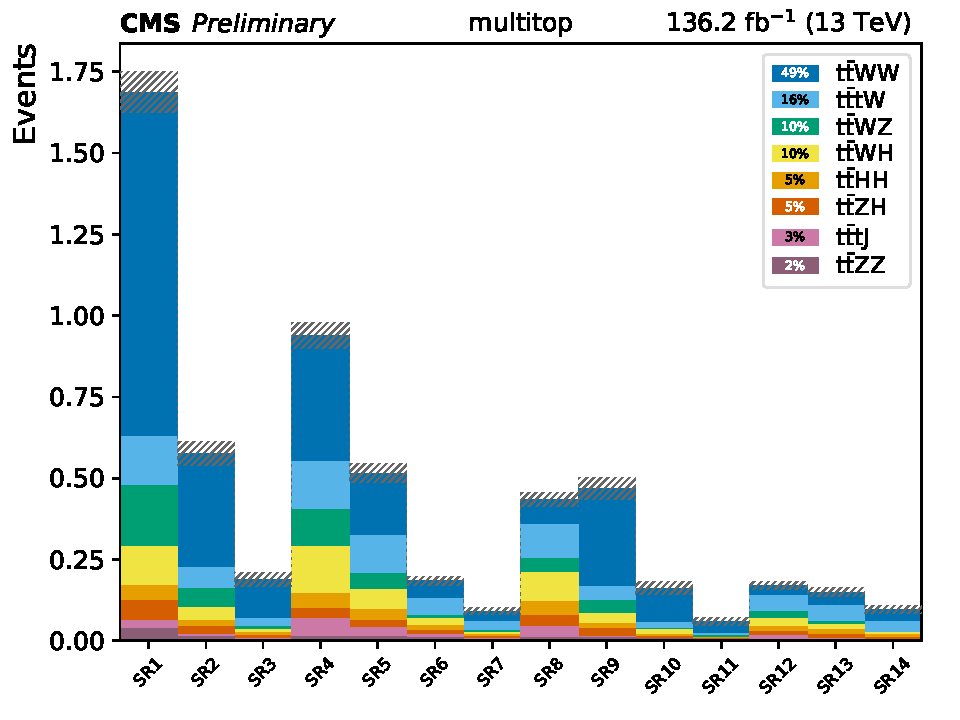
\includegraphics[width=.60\textwidth]{figs/ftan/h_multitop.pdf} \\
    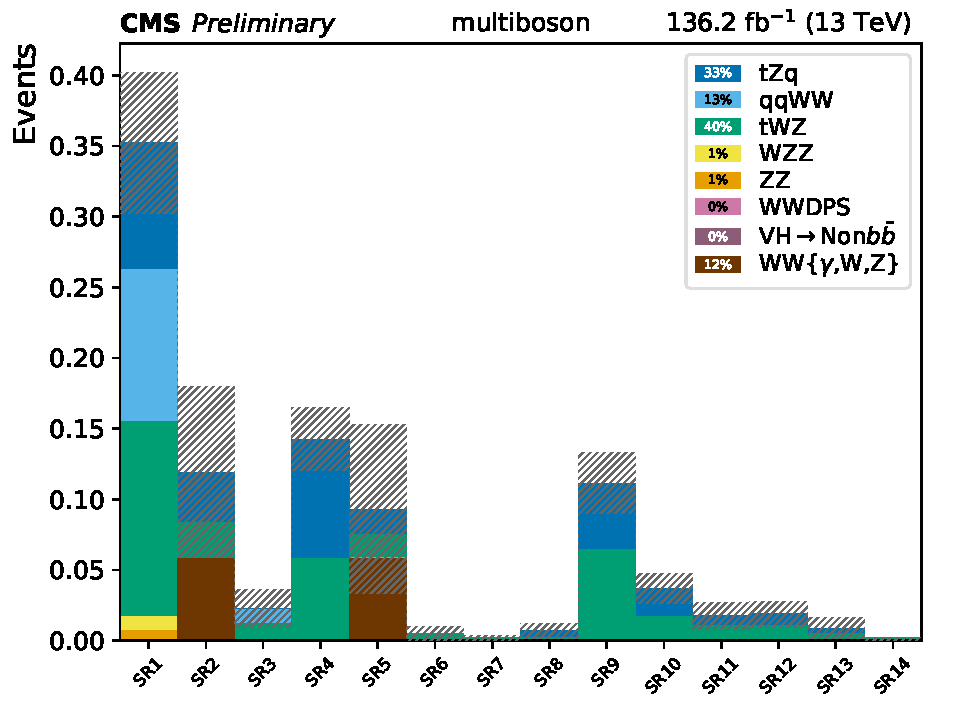
\includegraphics[width=.60\textwidth]{figs/ftan/h_multiboson.pdf}
    \caption{ Relative composition of multi-top (top) and multi-boson (bottom) rare backgrounds in the signal regions for all MC.}
    \label{fig:ftraressr}
\end{figure}

For the \smft analysis,
we apply uncertainties of 20\%, 11\%, and 11\% for Rare, \Xgamma, and \ttVV categories,
respectively, and 40\% for the \ttW and \ttZ categories. Also in the \smft analysis,
the \ttH category is assigned an uncertainty of 25\% to reflect the CMS \ttH 
measurement~\cite{CMS:Sirunyan2018hoz} which obtained a signal strength $\mu_{\ttH}$, defined
as the ratio between the measured $\ttH$ cross section and its SM expectation,
of $1.26^{+0.31}_{-0.26}$.

\FloatBarrier

\section{Nonprompt leptons}
\mytodo{todo}

\section{Charge misidentification}

The charge misidentification/flip background results from events that have
isolated OS leptons where the charge of one of the leptons is
misidentified due to mismeasurement (typical at high \pt) or bremsstrahlung.
Muons are relatively well-measured and less susceptible to radiation due to their
mass, so charge flips of muons are neglected compared to electrons.

The charge flip background is estimated by selecting OS $ee$ or $e\mu$ events 
which pass the appropriate baseline selection depending on analysis,
and then weighting the events by the \pt and $\eta$-dependent 
probability of electron charge mismeasurement, which is calculated from simulation.

The two-dimensional probability maps, shown for each of the three years of data collection 
in Fig.~\ref{fig:fliprate}, are obtained from a combination of
\ttbar and DY simulation. The probabilities
are then validated using a control sample in data of
SS $\PZ\rightarrow e^\pm e^\pm$ baseline events, 
instead using a $\ptmiss<50\GeV$ requirement to be
orthogonal to the signal regions. 
The level of disagreement in this control region
is used to assess the associated systematic uncertainty and to derive a
correction to the MC-based rate estimation.  In the 2016 data sample, we find good
agreement between prediction and data in the control region.
However, in the 2017 and 2018 data samples, the MC-based flip rate
is significantly lower than for
2016 due to the upgraded pixel detector (which added an extra inner pixel layer),
so the obsered number of events in the
SS $\PZ\rightarrow e^\pm e^\pm$ region is found to be nearly 40\% higher than the
predicted number of events. Consequently, the 2017 and 2018 charge
flip predictions are scaled up by approximately 40\%, as seen in
Figure~\ref{fig:flipclosure}. These year-by-year correction factors are summarized in
Table~\ref{tab:flipscaling}. Since we do not observe significant trends
in the lepton kinematics, we do not consider \pt and $\eta$-binned
corrections on top of the tabulated flat correction factors. 
In addition to the statistical uncertainties, we apply a 20\%
systematic uncertainty on this background prediction for all years. In MC, the
flip rate for muons is found to be an order of magnitude smaller than for
electrons and is therefore neglected, as it would in any case be covered by
the systematic uncertainty of 20\% on this background.



\begin{table}[h]
  \begin{center}
    \small
    \begin{tabular}{c|c}
      \hline
      year & observation/prediction \\
      \hline
        2016 & 1.01  \\
        2017 & 1.44  \\
        2018 & 1.41  \\
      \hline
    \end{tabular}
    \caption{ Ratio of observed flip rate in data to the flip rate prediction from simulation.
     These are the multiplicative correction to the MC-based charge flip probabilities. }
    \label{tab:flipscaling}
  \end{center}
\end{table}

\begin{figure}[!hbtp]
\centering
\centering
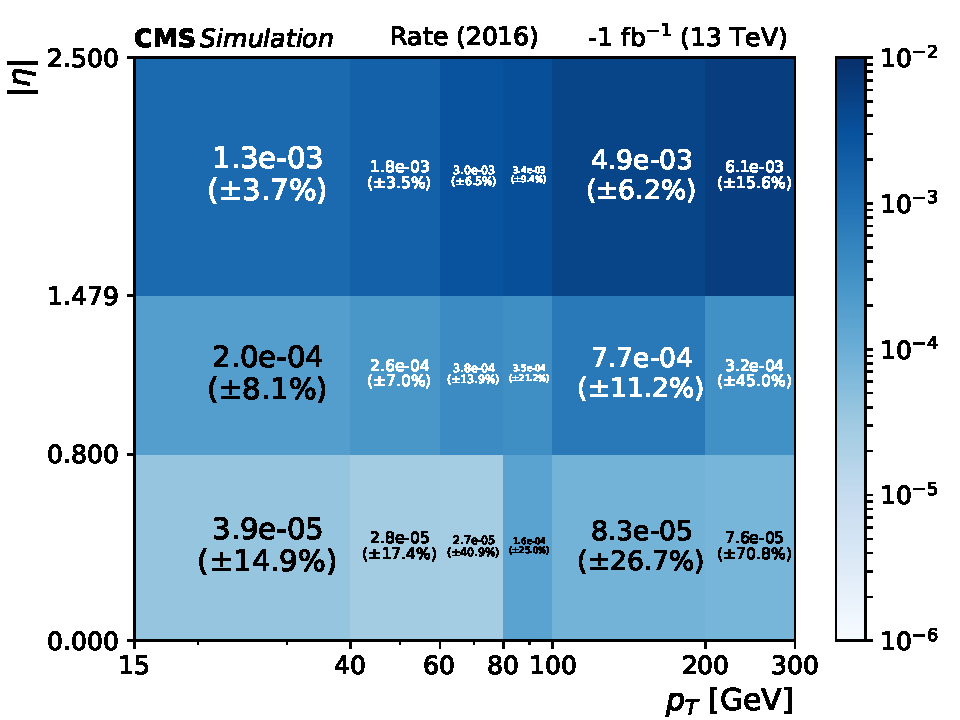
\includegraphics[width=.48\textwidth]{figs/ftan/flips/y2016/fliprate.pdf}
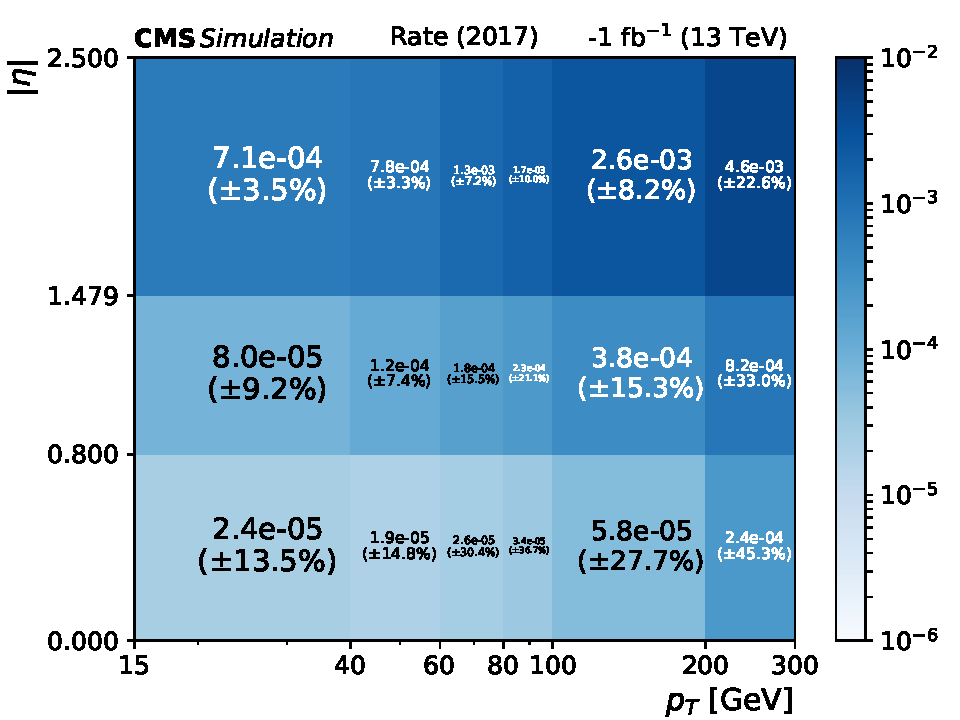
\includegraphics[width=.48\textwidth]{figs/ftan/flips/y2017/fliprate.pdf}
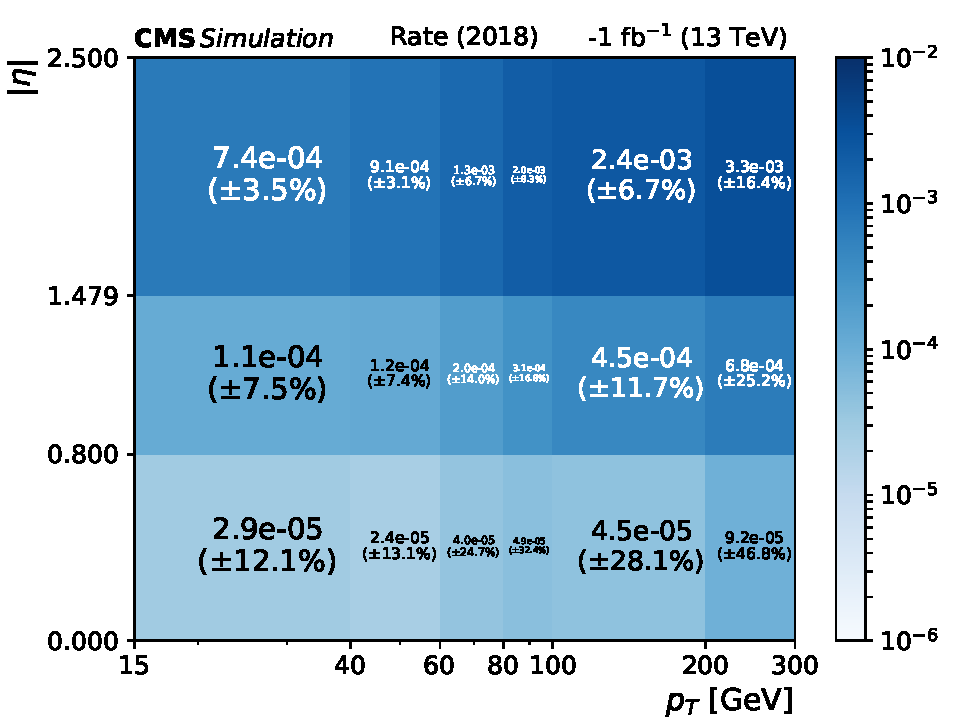
\includegraphics[width=.48\textwidth]{figs/ftan/flips/y2018/fliprate.pdf}
\caption{ Electron charge flip rate for 2016, 2017, and 2018. }
\label{fig:fliprate}
\end{figure}

\begin{figure}[!hbtp]
\centering
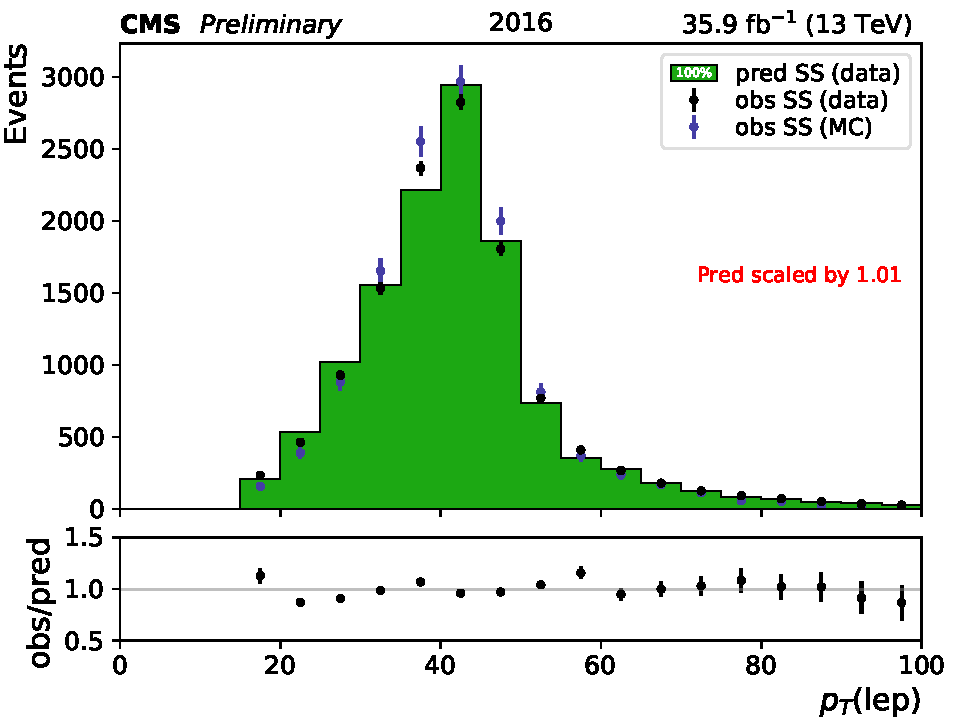
\includegraphics[width=.31\textwidth]{figs/ftan/flips/y2016/leppt.pdf}
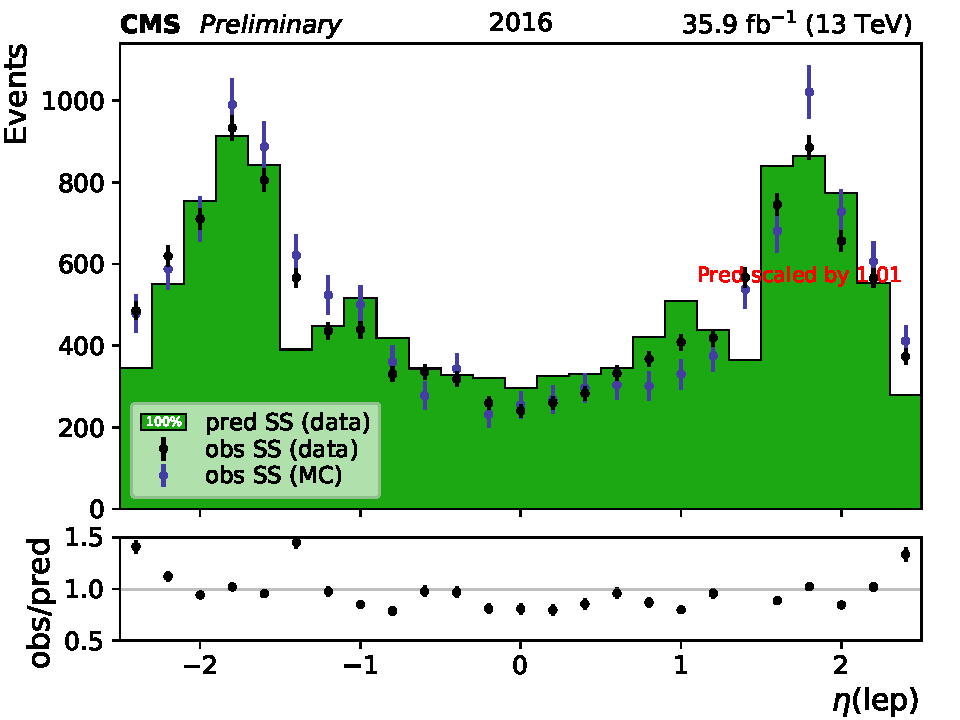
\includegraphics[width=.31\textwidth]{figs/ftan/flips/y2016/lepeta.pdf}
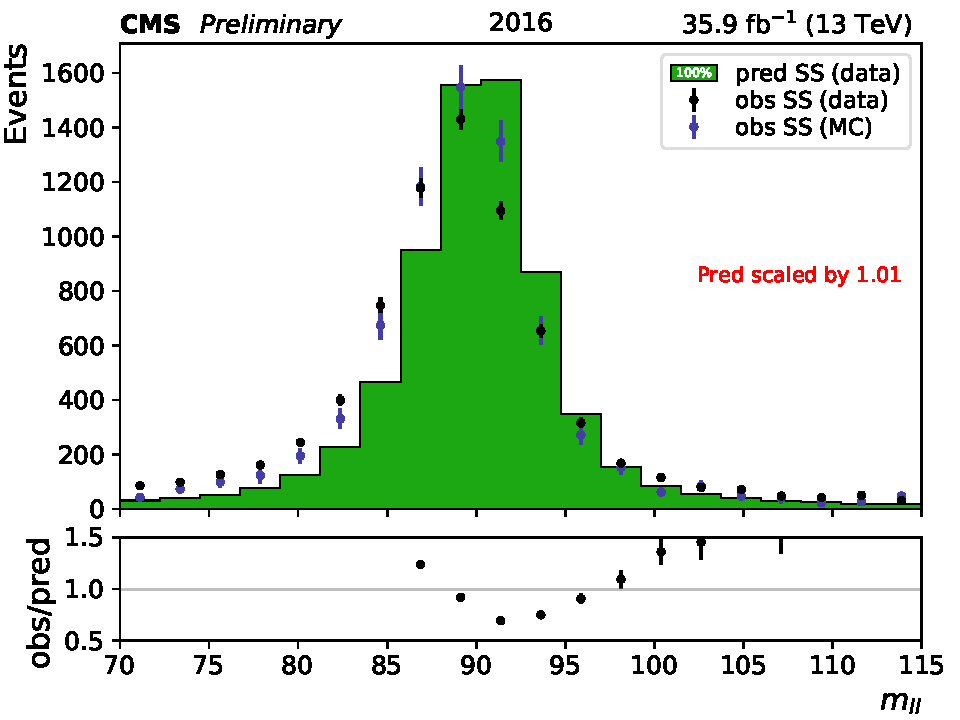
\includegraphics[width=.31\textwidth]{figs/ftan/flips/y2016/mll.pdf} \\
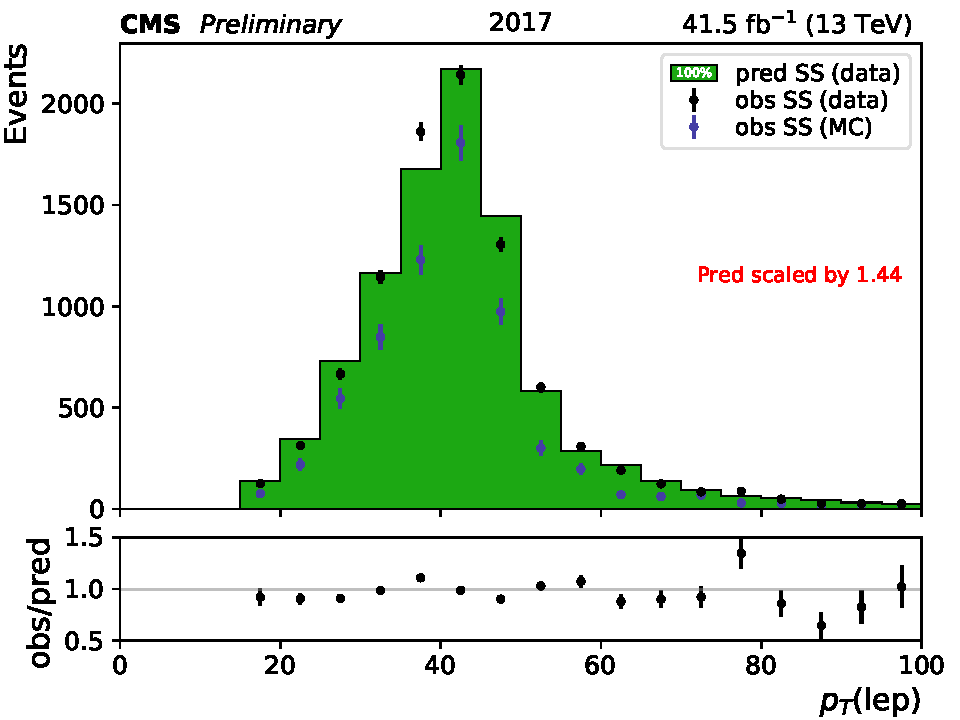
\includegraphics[width=.31\textwidth]{figs/ftan/flips/y2017/leppt.pdf}
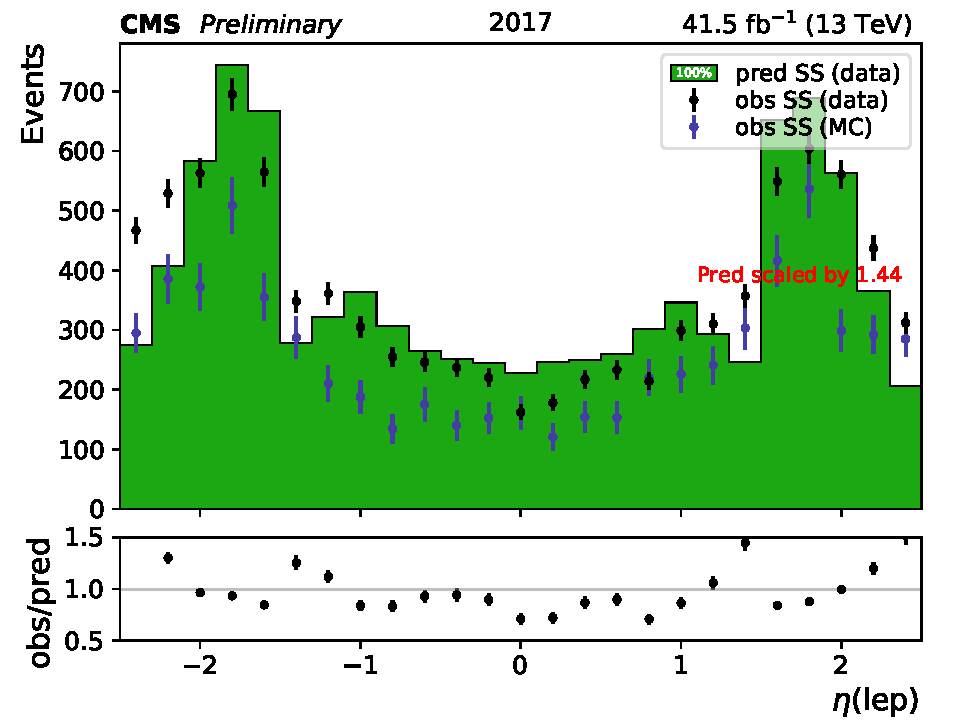
\includegraphics[width=.31\textwidth]{figs/ftan/flips/y2017/lepeta.pdf}
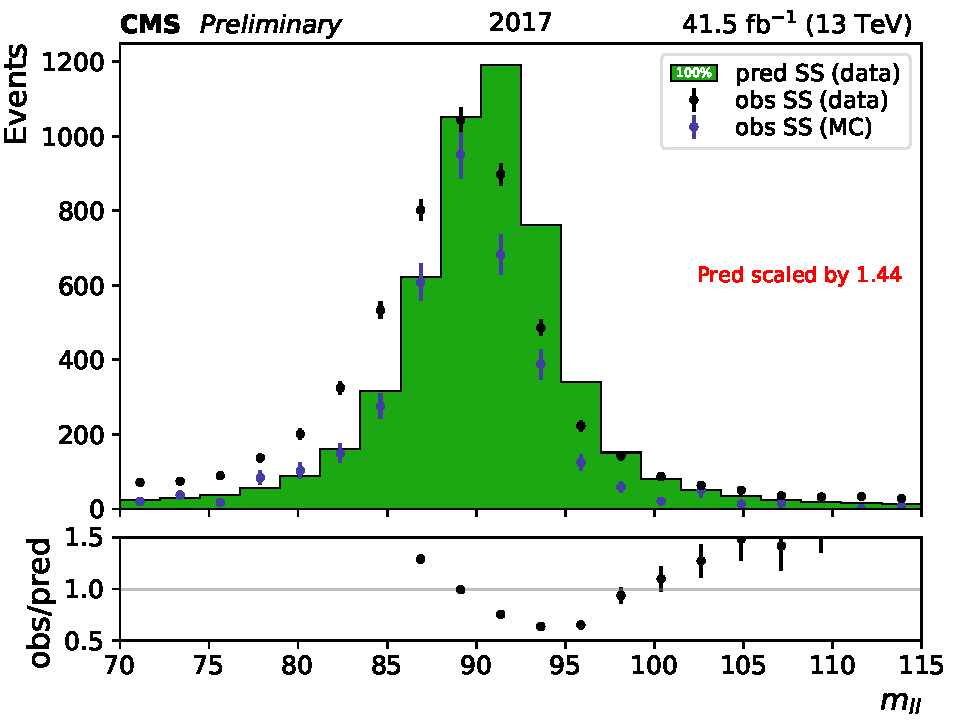
\includegraphics[width=.31\textwidth]{figs/ftan/flips/y2017/mll.pdf} \\
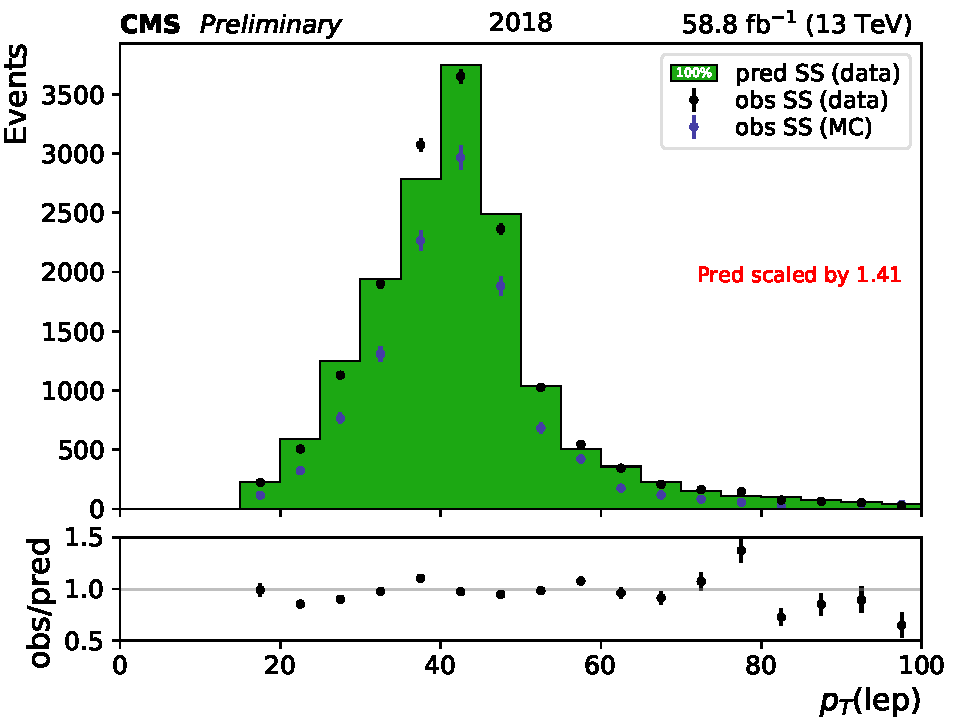
\includegraphics[width=.31\textwidth]{figs/ftan/flips/y2018/leppt.pdf}
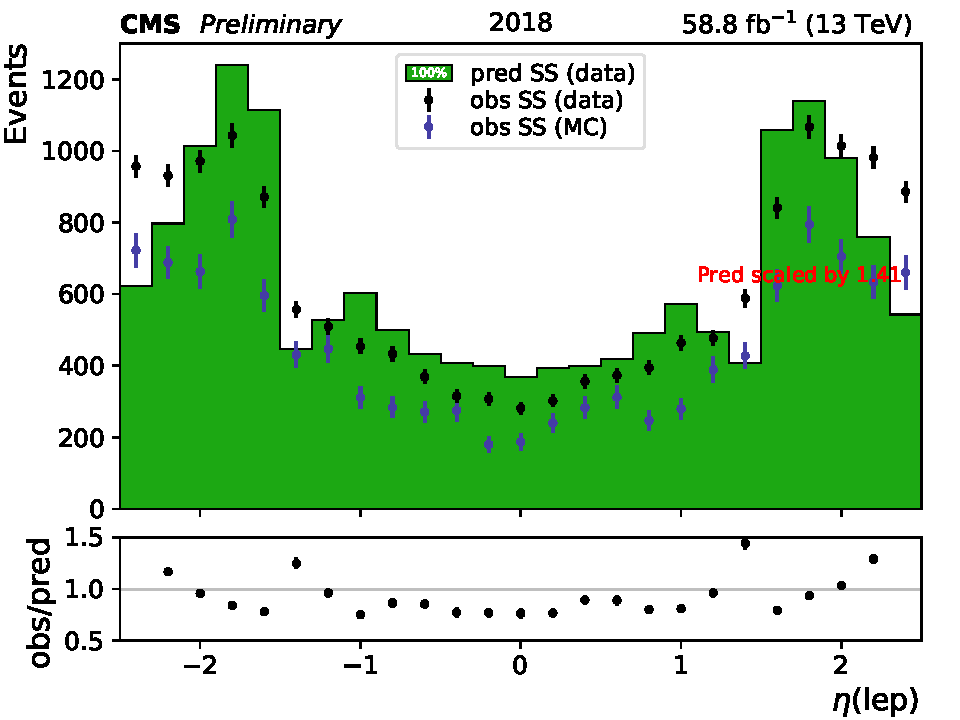
\includegraphics[width=.31\textwidth]{figs/ftan/flips/y2018/lepeta.pdf}
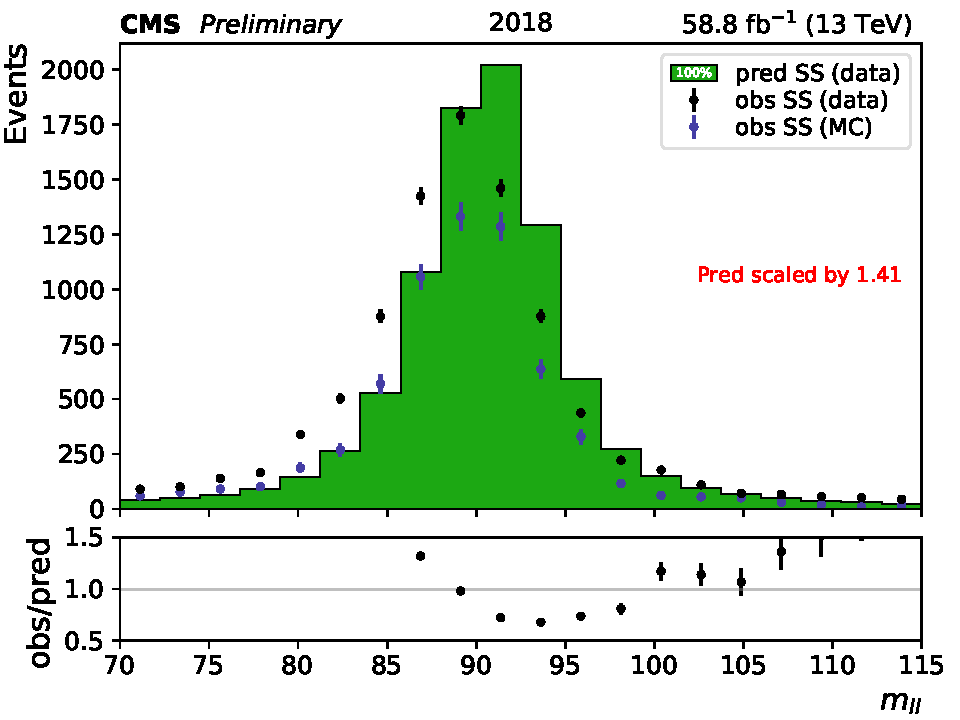
\includegraphics[width=.31\textwidth]{figs/ftan/flips/y2018/mll.pdf} \\
    \caption{  Predicted and observed lepton \pt (left) and $\eta$ (middle) and $m_{\ell\ell}$ (right) in a SS $\PZ \rightarrow e^\pm e^\pm$ peak
    for the years 2016, 2017, and 2018, from top to bottom.
The prediction is normalized to the observed data with the normalization factor inset in red.
The filled green histogram consists of predicted charge flip events (reweighted OS events),
the black points consist of observed charge flip events in data (SS), and the blue points
show the observed charge flip events in MC (SS).
}
\label{fig:flipclosure}
\end{figure}

\FloatBarrier

\section{Corrections}
\mytodo{todo}

In addition to corrections associated with JEC, \PQb-tagging, lepton scale factors,
and trigger scale factors, mentioned throughout previous sections and chapters, we
apply some dedicated corrections to simulation to bring better agreement between data
and simulation.

\mytodo{ttbb}

\mytodo{nisr}

\section{Control regions}
\mytodo{todo}

\section{Systematic uncertainties}
\mytodo{todo}

 % Background estimation
\chapter{Results and interpretations}
\label{sec:results}
\section{SUSY results}
\label{sec:ssresults}

\section{SUSY interpretations}
\label{sec:ssresults}

\section{Four top results}
\label{sec:ftresults}

Distributions of the main kinematic variables (\Njets, \Nbjets, \HT, and
\ptmiss) for events in the four top analysis baseline region are shown in Fig.~\ref{fig:kinemsr} and compared
to the SM background predictions. The \Njets and \Nbjets distributions for
the CRW and CRZ are shown in Fig.~\ref{fig:kinemcr}. The expected SM \tttt
signal, normalized to its predicted cross section, is shown in both figures.
The SM predictions are statistically consistent with the observations.

\begin{figure*}[!hbt]
\centering
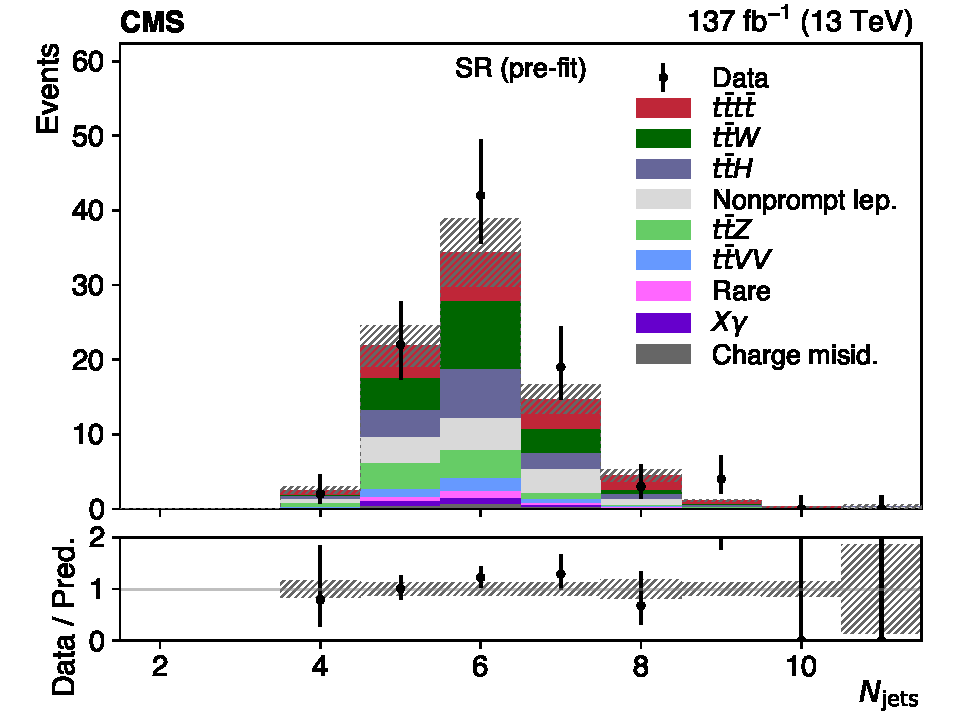
\includegraphics[width=.49\textwidth]{figs/ftp/sr_njets_prefit.pdf}
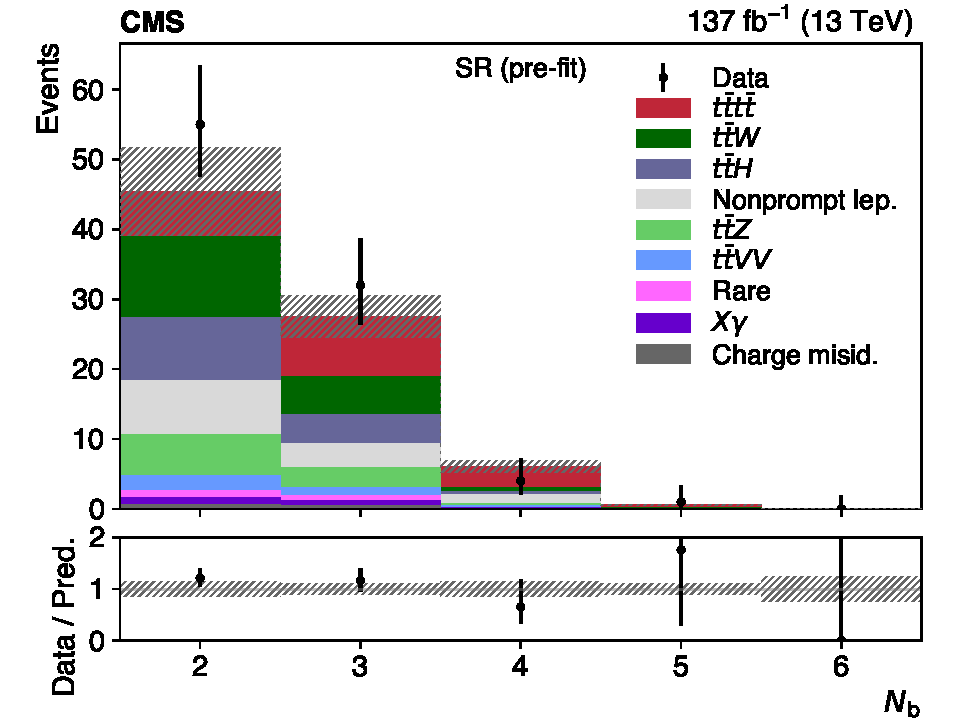
\includegraphics[width=.49\textwidth]{figs/ftp/sr_nbtags_prefit.pdf}
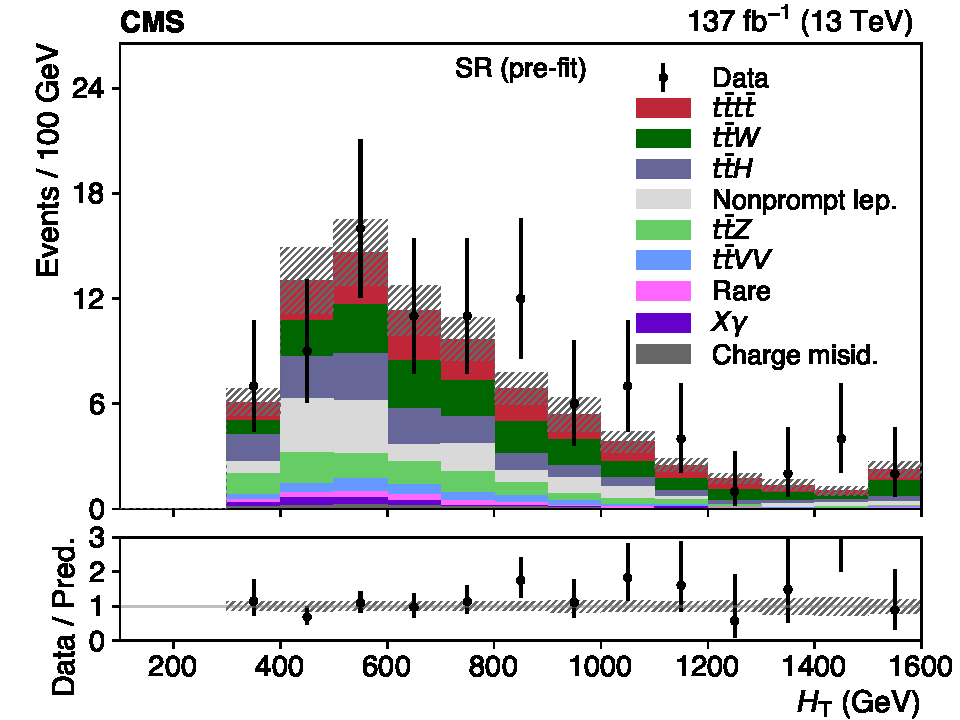
\includegraphics[width=.49\textwidth]{figs/ftp/sr_ht_prefit.pdf}
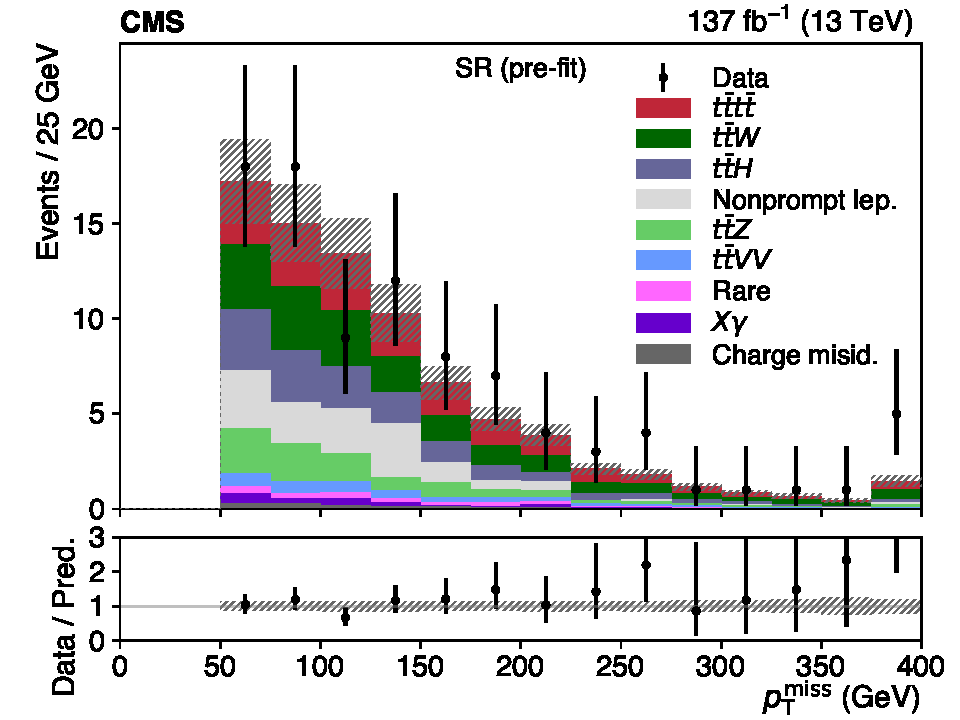
\includegraphics[width=.49\textwidth]{figs/ftp/sr_met_prefit.pdf}
\caption{ Distributions of \Njets (upper left), \Nbjets (upper right), \HT (lower left), and \ptmiss (lower right) in the summed SRs (1--14), before fitting to data,
where the last bins include the overflows. The hatched areas represent the total uncertainties in the SM signal and background predictions.
 The lower panels show the ratios of the observed event yield to the total prediction of
    signal plus background.
    }
\label{fig:kinemsr}
\end{figure*}

\begin{figure*}[!hbt]
\centering
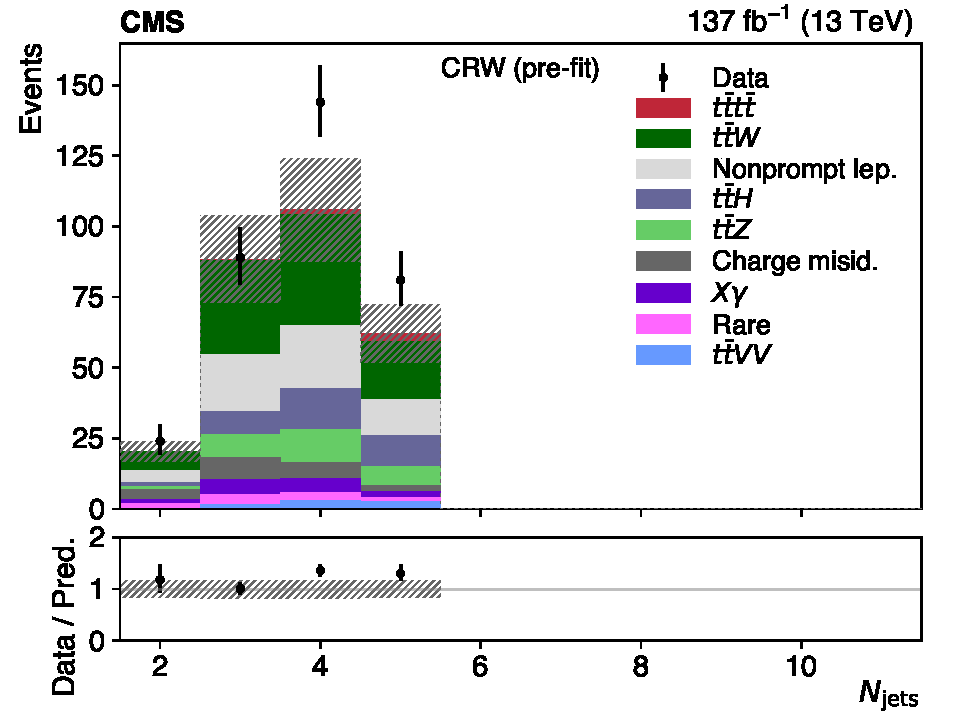
\includegraphics[width=.49\textwidth]{figs/ftp/ttwcr_njets_prefit.pdf}
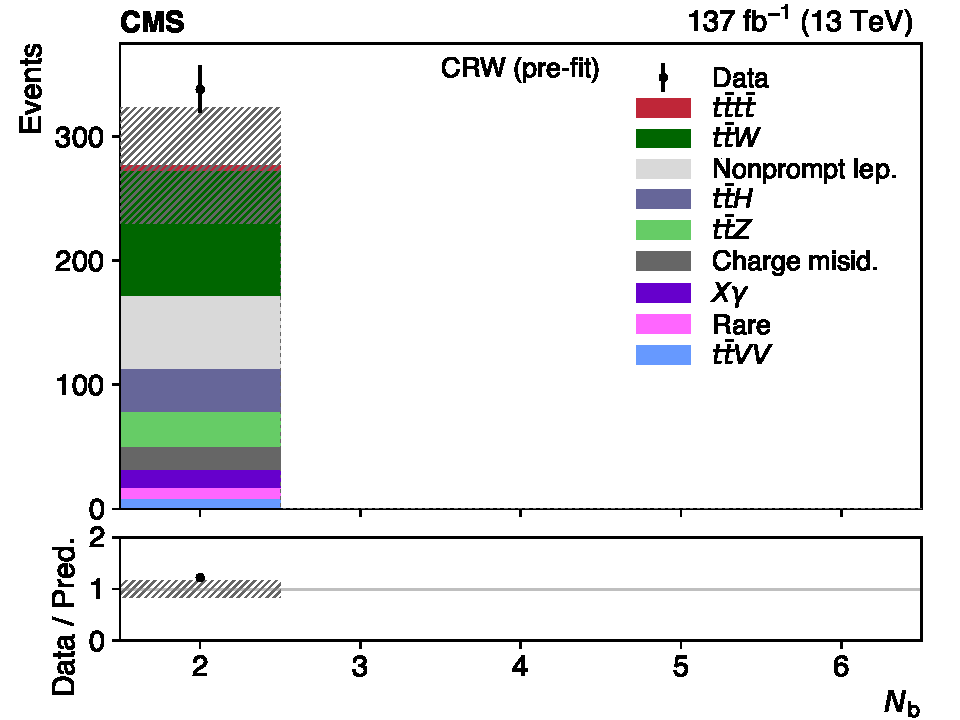
\includegraphics[width=.49\textwidth]{figs/ftp/ttwcr_nbtags_prefit.pdf}
\includegraphics[width=.49\textwidth]{figs/ftp/ttzcr_njets_prefit.pdf}
\includegraphics[width=.49\textwidth]{figs/ftp/ttzcr_nbtags_prefit.pdf}
    \caption{Distributions of \Njets (left) and \Nbjets (right) in the \ttW (upper) and \ttZ (lower) CRs, before fitting to data.
The hatched areas represent the  uncertainties in the SM signal and background predictions.
 The lower panels show the ratios of the observed event yield to the total prediction of
    signal plus background.
    }
\label{fig:kinemcr}
\end{figure*}

A binned likelihood is constructed using the yields from the signal regions,
the CRZ, as well as the CRW for the cut-based analysis only, incorporating
experimental and theoretical uncertainties as ``nuisance'' parameters. 
The measured cross
section for \tttt and the significance of the observation relative to the
background-only hypothesis are obtained from a profile maximum-likelihood
fit, in which the parameter of interest is \xsectttt and all nuisance
parameters are profiled, following the procedures described in
Refs.~\cite{STAT:ATLPHYSPUB2011011,STAT:PDG}. In addition, an upper limit at 95\%
confidence level (\CL) is set on \xsectttt using the modified frequentist
\CLs criterion~\cite{STAT:Junk1999kv,STAT:Read2002hq}, with the profile likelihood
ratio test statistic and asymptotic approximation~\cite{STAT:Cowan2010js}. We
verified the consistency between the asymptotic and fully toy-based methods.
Alternatively, by considering the SM, including the \tttt process with the SM
cross section and uncertainty~\cite{THEORY:Frederix2017wme}, as the null
hypothesis, the fit provides cross section upper limits on BSM processes with
new scalar and pseudoscalar particles.

The values and uncertainties of most nuisance parameters are unchanged by the
fit, but the ones significantly affected include those corresponding to the
\ttW and \ttZ normalizations, which are both scaled by $1.3\pm0.2$ by the
fit, in agreement with the ATLAS and CMS measurements of these
processes~\cite{ATLAS:Aaboud2019njj, CMS:Sirunyan2017uzs, CMS:2019too}. The
predicted yields after the maximum-likelihood fit (post-fit) are compared to
data in Fig.~\ref{fig:srcr} for the cut-based (upper) and BDT (lower)
analyses, where the fitted \tttt signal contribution is added to the
background predictions. The corresponding yields are shown in
Tables~\ref{tab:srcryields} and \ref{tab:srdiscyields} for the cut-based and
BDT analysis, respectively.

The \tttt cross section and the 68\% \CL interval is measured to be
$9.4^{+6.2}_{-5.6}\unit{fb}$ in the cut-based analysis, and
$12.6^{+5.8}_{-5.2}\unit{fb}$ in the BDT analysis. Relative to the
background-only hypothesis, the observed and expected significances are 1.7
and 2.5 standard deviations, respectively, for the cut-based analysis, and
2.6 and 2.7 standard deviations for the BDT analysis. The observed 95\% \CL
upper limits on the cross section are $20.0\unit{fb}$ in the cut-based and
$22.5\unit{fb}$ in the BDT analyses. The corresponding expected upper limits
on the \tttt cross section, assuming no SM \tttt contribution to the data,
are $9.4^{+4.3}_{-2.9}\unit{fb}$ (cut-based) and $8.5^{+3.9}_{-2.6}\unit{fb}$
(BDT), a significant improvement relative to the value of
$20.8^{+11.2}_{-6.9}\unit{fb}$ of Ref.~\cite{CMS:myTOP2016}. We consider the BDT
analysis as the primary result of this paper, as it provides a higher
expected measurement precision, and use the results from it for further
interpretations in the following section.




\begin{figure}[!hbtp]
\centering
\includegraphics[width=0.8\textwidth]{figs/ftp/SRCR_postfit.pdf} \\
\includegraphics[width=0.8\textwidth]{figs/ftp/SRDISC_postfit.pdf}
\caption{ Observed yields in the control and signal regions for the cut-based (upper) and BDT (lower) analyses,
compared to the post-fit predictions for signal and background processes.
The hatched areas represent the total post-fit uncertainties in the signal and background predictions.
The lower panels show the ratios of the observed event yield to the total prediction of
    signal plus background.
    }
\label{fig:srcr}
\end{figure}


\begin{table*}[htb!]
\centering
    \caption{
        The post-fit predicted background, $\tttt$ signal, and total yields with
          their total uncertainties and the observed number of events
          in the control and signal regions in data for the cut-based analysis.
}
\label{tab:srcryields}
    \begin{tabular}{ccccc}
        & SM background  & $\tttt$   & Total   & Observed \\
            \hline
CRZ  & $101\pm10\ \ $   & $0.83\pm0.49$ & $102\pm10\ \ $   & 104 \\
CRW  & $331\pm19\ \ $   & $3.9\pm2.3$   & $335\pm18\ \ $   & 338 \\
SR1  & $25.6\pm2.1\ \ $ & $2.0\pm1.2$   & $27.6\pm2.1\ \ $ & 33 \\
SR2  & $9.1\pm1.3$      & $1.13\pm0.65$ & $10.3\pm1.3\ \ $ & 9 \\
SR3  & $2.01\pm0.58$    & $0.73\pm0.42$ & $2.74\pm0.67$    & 3 \\
SR4  & $11.3\pm1.3\ \ $ & $1.58\pm0.90$ & $12.9\pm1.3\ \ $ & 14 \\
SR5  & $5.03\pm0.77$    & $1.68\pm0.95$ & $6.7\pm1.1$      & 5 \\
SR6  & $2.29\pm0.40$    & $1.20\pm0.67$ & $3.48\pm0.66$    & 8 \\
SR7  & $0.71\pm0.20$    & $0.88\pm0.48$ & $1.59\pm0.49$    & 0 \\
SR8  & $3.31\pm0.95$    & $2.2\pm1.3$   & $5.5\pm1.3$      & 5 \\
SR9  & $6.84\pm0.80$    & $0.71\pm0.39$ & $7.55\pm0.80$    & 6 \\
SR10 & $2.10\pm0.31$    & $0.35\pm0.22$ & $2.45\pm0.35$    & 3 \\
SR11 & $1.38\pm0.75$    & $0.23\pm0.14$ & $1.61\pm0.75$    & 1 \\
SR12 & $2.03\pm0.48$    & $0.59\pm0.34$ & $2.62\pm0.54$    & 2 \\
SR13 & $1.09\pm0.28$    & $0.69\pm0.39$ & $1.78\pm0.44$    & 2 \\
SR14 & $0.87\pm0.30$    & $0.80\pm0.45$ & $1.67\pm0.52$    & 1 \\
\end{tabular}
\end{table*}




\begin{table*}[htb!]
\centering
    \caption{
        The post-fit predicted background and $\tttt$ signal, and total yields with
          their total uncertainties and the observed number of events
          in the control and signal regions in data for the BDT analysis.
}
\label{tab:srdiscyields}
    \begin{tabular}{ccccc}
        & SM background  & $\tttt$   & Total   & Observed \\
            \hline

CRZ  & $102\pm12\ \ $   & $1.11\pm0.43$ & $103\pm12\ \ $   & 104 \\
SR1  & $3.95\pm0.96$    & $ <0.01 $     & $3.96\pm0.96$    & 4 \\
SR2  & $14.2\pm1.8\ \ $ & $0.01\pm0.01$ & $14.2\pm1.8\ \ $ & 19 \\
SR3  & $25.5\pm3.5\ \ $ & $0.04\pm0.03$ & $25.6\pm3.5\ \ $ & 19 \\
SR4  & $34.0\pm4.0\ \ $ & $0.08\pm0.05$ & $34.0\pm4.0\ \ $ & 33 \\
SR5  & $36.7\pm4.0\ \ $ & $0.15\pm0.07$ & $36.8\pm4.0\ \ $ & 36 \\
SR6  & $39.8\pm4.2\ \ $ & $0.23\pm0.12$ & $40.0\pm4.2\ \ $ & 44 \\
SR7  & $40.3\pm3.7\ \ $ & $0.31\pm0.16$ & $40.6\pm3.8\ \ $ & 41 \\
SR8  & $47.3\pm4.3\ \ $ & $0.72\pm0.28$ & $48.0\pm4.3\ \ $ & 46 \\
SR9  & $58.5\pm5.2\ \ $ & $1.18\pm0.46$ & $59.7\pm5.2\ \ $ & 48 \\
SR10 & $52.1\pm4.3\ \ $ & $1.91\pm0.74$ & $54.1\pm4.2\ \ $ & 61 \\
SR11 & $43.0\pm3.5\ \ $ & $3.0\pm1.2$   & $46.0\pm3.5\ \ $ & 62 \\
SR12 & $32.1\pm3.0\ \ $ & $3.7\pm1.4$   & $35.8\pm2.9\ \ $ & 40 \\
SR13 & $16.7\pm1.6\ \ $ & $4.3\pm1.6$   & $21.0\pm2.0\ \ $ & 15 \\
SR14 & $10.1\pm1.2\ \ $ & $4.2\pm1.6$   & $14.3\pm1.8\ \ $ & 16 \\
SR15 & $5.03\pm0.77$    & $4.1\pm1.5$   & $9.1\pm1.6$      & 4 \\
SR16 & $2.49\pm0.61$    & $3.4\pm1.3$   & $5.9\pm1.3$      & 7 \\
SR17 & $0.57\pm0.36$    & $1.08\pm0.42$ & $1.65\pm0.50$    & 3 \\

\end{tabular}

\end{table*}

\section{Four top interpretations}
\label{sec:ftinterpretations}

This analysis is used to constrain SM parameters, as well as production of
BSM particles and operators that can affect the \tttt production rate. The
existence of \tttt Feynman diagrams with virtual Higgs bosons allows
interpreting the upper limit on \xsectttt as a constraint on the Yukawa
coupling, $y_{\PQt}$, between the top quark and the Higgs
boson~\cite{THEORY:TopYukawaTTTT, THEORY:TopYukawaTTTTnew}. Similarly, the
measurement can be interpreted as a constraint on the Higgs boson oblique
parameter $\hat{H}$, defined as the Wilson coefficient of the dimension-six
BSM operator modifying the Higgs boson propagator~\cite{THEORY:ObliqueHiggs2019}.
More generically, Feynman diagrams where the virtual Higgs boson is replaced
by a virtual BSM scalar ($\phi$) or vector ($\cPZpr$) particle with mass
smaller than twice the top quark mass ($m < 2m_\PQt$), are used to interpret
the result as a constraint on the couplings of such new
particles~\cite{THEORY:Alvarez2016nrz}. In addition, new particles with $m >
2m_\PQt$, such as a heavy scalar (\PH) or pseudoscalar (\PSA), can be
produced on-shell in association with top quarks. They can subsequently decay
into top quark pairs, generating final states with three or four top quarks.
Constraints on the production of such heavy particles can be interpreted in
terms of 2HDM parameters~\cite{THEORY:Dicus1994bm,THEORY:Craig2015jba,THEORY:Craig2016ygr},
or in the framework of simplified models of dark matter~\cite{THEORY:Boveia2016mrp,
THEORY:Albert2017onk}.

When using our \tttt to determine a constraint on $y_{\PQt}$, we verified
using a LO simulation that the signal acceptance is not affected by the
relative contribution of the virtual Higgs boson Feynman diagrams. We take
into account the dependence of the backgrounds on $y_{\PQt}$ by scaling the
\ttH cross section by $\abs{y_{\PQt}/y_{\PQt}^{\mathrm{SM}}}^2$ prior to the
fit, where $y_{\PQt}^{\mathrm{SM}}$ represents the SM value of the top quark
Yukawa coupling. As a result of the \ttH background rescaling, the measured
\xsectttt depends on $\abs{y_{\PQt}/y_{\PQt}^{\mathrm{SM}}}$, as shown in
Fig.~\ref{fig:yukawa}. The measurement is compared to the theoretical
prediction obtained from the LO calculation of Ref.~\cite{THEORY:TopYukawaTTTT},
scaled to the $12.0^{+2.2}_{-2.5}\unit{fb}$ cross section obtained in
Ref.~\cite{THEORY:Frederix2017wme}, and including the uncertainty associated with
doubling and halving the renormalization and factorization scales. Comparing
the observed limit on \xsectttt with the central, upper, and lower values of
its theoretical prediction, we obtain 95\% \CL limits of
$\abs{y_{\PQt}/y_{\PQt}^{\mathrm{SM}}} < 1.7$, $1.4$, and $2.0$,
respectively, an improvement over the previous CMS
result~\cite{CMS:myTOP2016}. Alternatively, assuming that the on-shell Yukawa
coupling is equal to that of the SM, we do not rescale the \ttH background
with respect to its SM prediction, and obtain corresponding limits on the
off-shell Yukawa coupling of $\abs{y_{\PQt}/y_{\PQt}^{\mathrm{SM}}} < 1.8$,
$1.5$, and $2.1$. Since $y_{\PQt}$ affects the Higgs boson production cross
section in both the gluon fusion and \ttH modes, constraints on $y_{\PQt}$
can also be obtained from a combination of Higgs boson
measurements~\cite{STAT:AtlasCmsHiggsComb}. However, these constraints require
assumptions about the total width of the Higgs boson, while the \tttt-based
limit does not. For the $\hat{H}$ interpretation, the BDT analysis is
repeated using simulated samples of \tttt signal events with different values
of $\hat{H}$ to account for small acceptance and kinematic differences. 
We rescale the \ttH cross section by
$(1-\hat{H})^2$ to account for its $\hat{H}$
dependency~\cite{THEORY:ObliqueHiggs2019}. This results in the 95\% \CL upper limit
of $\hat{H} < 0.12$. For reference, the authors of
Ref.~\cite{THEORY:ObliqueHiggs2019} used recent LHC on-shell Higgs boson
measurements to set a constraint of $\hat{H} < 0.16$ at 95\% \CL.


To study the off-shell effect of new particles with $m < 2m_\PQt$, we first
consider neutral scalar ($\phi$) and neutral vector ($\cPZpr$) particles that
couple to top quarks. Such particles are at present only weakly constrained,
while they can give significant contributions to the \tttt cross
section~\cite{THEORY:Alvarez2016nrz}. Having verified in LO simulation that these
new particles affect the signal acceptance by less than 10\%, we recalculate
the \xsectttt upper limit of the BDT analysis including an additional 10\%
uncertainty in the acceptance, and obtain the 95\% \CL upper limit of
23.0\unit{fb} on the total \tttt cross section, slightly weaker than the
22.5\unit{fb} limit obtained in Section~\ref{sec:results}. Comparing this
upper limit to the predicted cross section in models where \tttt production
includes a $\phi$ or a $\cPZpr$ in addition to SM contributions and
associated interference, we set limits on the masses and couplings of these
new particles, shown in Fig.~\ref{fig:ZprimePhiExclusions}. These limits
exclude couplings larger than 1.2 for $m_{\phi}$ in the 25--340\GeV range and
larger than 0.1 (0.9) for $m_{\cPZpr} = 25$ (300)\GeV.

We consider on-shell effects from new scalar and pseudoscalar particles with $m > 2m_\PQt$. At such masses, the production rate of these particles
in association with a single top quark ($\PQt\PQq\PH/\PSA$, $\PQt\PW\PH/\PSA$) becomes significant,
so we include these processes in addition to $\PQt\overline{\PQt}\PH/\PSA$.
As pointed out in Ref.~\cite{THEORY:Craig2016ygr}, these processes do not suffer significant interference with the SM \tttt process.
To obtain upper limits on the sum of these processes followed by the decay $\PH/\PSA\to \ttbar$,
we use the BDT analysis and treat the SM \tttt process as a background.
Figure~\ref{fig:HiggsLimits} shows the excluded cross section as a function of the mass of the scalar (left) and pseudoscalar (right).
Comparing these limits with the Type-II 2HDM cross sections with $\tan\beta = 1$ in the alignment limit,
we exclude scalar (pseudoscalar) masses up to 470~(550)\GeV, improving by more than 100\GeV with respect to the previous CMS limits~\cite{CMS:mySUS2016}.
Alternatively, we consider the simplified model of dark matter defined in Ref.~\cite{CMS:DMsingletop},
which includes a Dirac fermion dark matter candidate, $\chi$, in addition to $\PH/\PSA$, and where the couplings of $\PH/\PSA$
to SM fermions and $\chi$ are determined by parameters $g_\mathrm{SM}$ and $g_\mathrm{DM}$, respectively.
In this model, exclusions similar to those from 2HDM are reached by assuming $g_\mathrm{SM} = 1$ and $g_\mathrm{DM} = 1$,
and taking  $m_{\PH/\PSA} < 2 m_\chi$.
Relaxing the 2HDM assumption of $\tan\beta = 1$, Fig.~\ref{fig:HiggsLimitsTB} shows the 2HDM limit as a function of $\PH/\PSA$ mass and $\tan\beta$,
considering one new particle at a time and also including a scenario with  $m_\PH = m_\PSA$ inspired by
a special case of Type-II 2HDM, the hMSSM~\cite{THEORY:Djouadi2013uqa}.
Values of $\tan\beta$ up to 0.8--1.6 are excluded, depending on the assumptions made.
These exclusions are comparable to those of a recent CMS search for the resonant production of $\PH/\PSA$ in the
$\Pp\to \PH/\PSA \to \ttbar$ channel~\cite{CMS:HIG17027}.
Relaxing the $m_{\PH/\PSA} < 2 m_\chi$ assumption in the dark matter model, Fig.~\ref{fig:DMLimits} shows the
limit in this model as a function of the masses of both $\PH/\PSA$ and $\chi$,
for $g_\mathrm{DM} = 1$ and for two different assumptions of $g_\mathrm{SM}$.
Large sections of the phase space of simplified dark matter models are excluded, and the reach of this analysis is complementary
to that of analyses
considering decays of $\PH/\PSA$ into invisible dark matter candidates, such as those of Refs.~\cite{CMS:DMsingletop, ATLAS:Aaboud2017rzf}.

\begin{figure}[!hbtp]
\centering
\includegraphics[width=.49\textwidth]{figs/ftp/yukawa.pdf}
\\
\caption{
    The observed \xsectttt (solid line) and 95\% \CL upper limit (hatched line) are shown as a function
    of $\abs{y_{\PQt}/y_{\PQt}^{\mathrm{SM}}}$. The predicted value (dashed line)~\cite{THEORY:TopYukawaTTTT},
    calculated at LO and scaled to the calculation from Ref.~\cite{THEORY:Frederix2017wme}, is also plotted.
    The shaded band around the measured value gives the total uncertainty, while the shaded band around
    the predicted curve shows the theoretical uncertainty associated with the renormalization and
    factorization scales.
}
\label{fig:yukawa}
\end{figure}

\begin{figure}[!hbtp]
\centering
    \includegraphics[width=.49\textwidth]{figs/ftp/plot_2d_phizprime.pdf}
\caption{
    The 95\% \CL exclusion regions in the plane of the $\phi/\cPZpr$-top quark coupling versus
    $m_{\phi}$ or $m_{\cPZpr}$. The excluded regions are above the hatched lines.
    }
\label{fig:ZprimePhiExclusions}
\end{figure}

\begin{figure*}[!hbtp]
\centering
    \includegraphics[width=.49\textwidth]{figs/ftp/ft_higgs_sc_scan_limit.pdf}
    \includegraphics[width=.49\textwidth]{figs/ftp/ft_higgs_ps_scan_limit.pdf}
\caption{
    The observed (points) and expected (dashed line) 95\% \CL upper limits on the cross section
    times branching fraction to \ttbar for the production of a new heavy scalar \PH (left) and pseudoscalar \PSA (right),
    as a function of mass. The inner and outer bands around the expected limits indicate the regions containing 68 and 95\%,
    respectively, of the distribution of limits under the background-only hypothesis. Theoretical values are shown for Type-II 2HDM
    in the alignment limit (solid line) and simplified dark matter (dot-dashed line) models.
}
\label{fig:HiggsLimits}
\end{figure*}

\begin{figure*}[!hbtp]
\centering
    \includegraphics[width=.49\textwidth]{figs/ftp/plot_2d_2hdm_tanbetaexclusion_h.pdf}
    \includegraphics[width=.49\textwidth]{figs/ftp/plot_2d_2hdm_tanbetaexclusion_a.pdf}
    \includegraphics[width=.49\textwidth]{figs/ftp/plot_2d_2hdm_tanbetaexclusion_b.pdf}
\caption{
    The observed (solid curve) and expected (long-dashed curve) 95\% \CL exclusion regions in the $\tan\beta$ versus mass plane
    for Type-II 2HDM models in the alignment limit for a new scalar \PH (upper left), pseudoscalar \PSA (upper right), and both (lower) particles.
    The short-dashed curves around the expected limits indicate the region containing 68\% of the distribution of limits expected under the
    background-only hypothesis. The excluded regions are below the curves.
}
\label{fig:HiggsLimitsTB}
\end{figure*}

\begin{figure*}[!hbtp]
\centering
    \includegraphics[width=.49\textwidth]{figs/ftp/plot_2d_dmscalar_xsec_totsm_bothcouplings.pdf}
    \includegraphics[width=.49\textwidth]{figs/ftp/plot_2d_dmpseudo_xsec_totsm_bothcouplings.pdf}
\caption{
	Exclusion regions at 95\% \CL in the plane of $m_\chi$ vs. $m_{\PH}$ (left) or $m_{\PSA}$ (right).
    The outer lighter and inner darker solid curves show the expected and observed limits, respectively,
    assuming $g_\mathrm{SM} = g_\mathrm{DM} = 1$. The excluded regions, shaded, are above the limit curves.
    The dashed lines show the limits assuming a weaker coupling between $\PH/\PSA$ and $\chi$, $g_\mathrm{DM} = 0.5$.
    }
\label{fig:DMLimits}
\end{figure*}
 % Results and interpretations
\chapter{Summary and conclusions}
\label{chap:summary}

A sample of events with two same-sign or at least three charged leptons
produced in association with several jets in proton-proton collisions at
13\TeV, corresponding to an integrated luminosity of \sslumi, has been
studied to search for physics beyond the standard model, as well as for the
standard model (SM) production of four top quarks.

In the inclusive BSM analysis, no significant excesses were found and the
results are interpreted as limits on cross sections at 95\% confidence level
for the production of new particles in simplified supersymmetric models,
considering both R parity conserving and violating scenarios. The limits
are translated into lower mass limits that are as large as 2.1\TeV for
gluinos and 0.9\TeV for top and bottom squarks. 
To assist with future re-interpretations, model-independent limits are
provided as a function of the missing transverse momentum and the scalar sum
of jet transverse momenta in an event.

The SM four top quark production search analyzed the dataset using two
strategies, the first relying on a cut-based categorization in lepton
multiplicity, jet multiplicity, and jet flavor, and the second taking
advantage of a boosted decision tree (BDT) to distinguish the \tttt signal
from backgrounds. The more precise multivariate strategy yields an observed
(expected) significance of 2.6 (2.7) standard deviations relative to the
background-only hypothesis, and a measured value for the \tttt cross section
of $12.6^{+5.8}_{-5.2}~\unit{fb}$. The results based on the two strategies are
in agreement with the SM prediction of $12.0^{+2.2}_{-2.5}~\unit{fb}$. The
results of the BDT approach are used to constrain the top quark Yukawa
coupling, $y_{\PQt}$, resulting in the 95\% confidence level (\CL) limit of
$\abs{y_{\PQt}/y_{\PQt}^{\mathrm{SM}}} < 1.7$. The Higgs boson oblique
parameter in the effective field theory
framework~\cite{THEORY:ObliqueHiggs2019} is similarly constrained to $\hat{H}
< 0.12$ at 95\% \CL. Upper limits between 0.1 and 1.2 are also set on the
coupling between the top quark and a new scalar ($\phi$) or vector ($\cPZpr$)
particle with mass less than twice that of the top quark
($m_\PQt$)~\cite{THEORY:Alvarez2016nrz}. Considering new scalar or
pseudoscalar particles with $m > 2m_\PQt$, and decaying to \ttbar,
their production in association with one or two top quarks is probed.
The resulting cross section upper limit, between 15 and
35~\unit{fb} at 95\% \CL, is interpreted in the contexts of Type-II
two-Higgs-doublet models and simplified dark matter models.

What a mouthful! In other words, the meta-summary is: the data collected by
the CMS detector from 2016 to 2018 did not turn up any interesting hints of
new physics in the same-sign final state. However, in the coming years, the
High-Luminosity LHC project seeks to at least double the dataset size
analyzed here. This will undoubtedly allow SM \tttt measurement to pass the
3-$\sigma$ evidence threshold, and maybe we will see hints of new physics.

 % Summary and conclusions

%=== Appendix ============================================
\appendix

\dsp

\mytodo{appendix on hem issue?}
\chapter{Statistics}
\label{appendix:statistics}

\begin{section}{Toy profile likelihood}


This section presents an introduction to the profile likelihood method
(used for the statistical results of this thesis) with a concrete toy example.
The toy example consists of one signal, one background, and one shape-based
nuisance parameter. Complete details of the method are in Reference~\cite{STAT:Cowan2010js}.


\begin{subsection}{Terminology}

Bayes' theorem can be stated in a more applicable way as
\begin{equation}
p(k|D) = \frac{p(D|k)p(k)}{p(D)}
\end{equation}
where $p(A|B)$ is the (conditional) probability of A given B.
Here, $k$ represents a model, which consists of a set of parameters 
(parameters of interest, as well as annoying/nuisance parameters). 
Typically, the single parameter of interest is a signal ``strength'' $\mu$
    (how much signal is there actually, compared to what is nominally in the simulation -- $\mu = \mu_\mathrm{obs}/\mu_\mathrm{SM}$), 
 and a set of (many) nuisance parameters technically specified
as a vector $\vec{\theta}$, but often just $\theta$. The posterior probability 
distribution function (pdf), $p(k|D)$ is the distribution of parameters given the observed
data D. The \textbf{likelihood} $p(D|k)$ gives the likelihood of getting some data $D$
given a particular model encoded in $k$. $p(k)$ is a prior distribution of models, often
taken to be ``flat'' in $\mu$. Lastly, the overall constant $p(D)$ is ignorable when dealing
with differences in likelihoods.

Analysis observables are typically binned into many regions, and compared with an observed count (data).
Integral data event counts (N) obey Poisson statistics, where $\lambda$ governs the underlying
rate of a process: $p(N|\lambda) = e^{-\lambda}\frac{\lambda^N}{N!}$ .
(Although, when statistics are large, Gaussian approximations can be made in order to simplify computations.)
For independent bins, the likelihood is a product over each of the bins.

This sets the stage for the toy example, which clarifies the meaning of the word \textbf{profile}.



\end{subsection}

\begin{subsection}{Toy example}

Figure~\ref{fig:toystat:njets} shows a toy distribution of jet multiplicity
for background, signal, and data. The background component also contains a
systematic uncertainty band corresponding to a shape nuisance parameter.
This shape nuisance parameter prefers to increase yields at higher number of jets.

\begin{figure}[!htb]
    \centering
    \includegraphics[width=0.48\linewidth]{figs/toy_statistics/njets.pdf}
    \includegraphics[width=0.48\linewidth]{figs/toy_statistics/backgroundvariations.pdf}
    \caption{
Toy distribution (left) and single shape nuisance variation on background component (right)
    }
    \label{fig:toystat:njets}
\end{figure}
    
As an intermediate goal to most statistical results/interpretations of the data,
we want to compute the likelihood which will be a 2D function of the
signal strength $\mu$ and the value of the systematic variation
$\theta$. $\theta=0$ will give the normal background yields, while
$\theta=-1$ and $\theta=1$ will give the $1\sigma$ down and up
variations, respectively. From above, $\theta=1$ will absorb
 the signal, as it increases the background yield at high number of
jets.

The likelihood function is the binned probability to get the data from a
$b$ (background-only) or $s+b$ (background and signal) poisson distribution, 
accounting for the probability of nuisances $\theta$ with the pdf $p(\theta)$:
\begin{equation}
\mathcal{L}(\mathrm{data}|\mu,\theta)=\prod_{j\in\mathrm{bins}}
\frac{(\mu s_j + b_j)^{n_j}}{n_j!}
e^{-(\mu s_j + b_j)}
p(\theta)
\end{equation}
 here $n_j$ represents the data count in bin $j$, $b_j$ the
background count, and $s_j$ the signal count. Technically, $b_j$ is
a function of $\theta$; that is, $b_j(\theta)$ depends on the value
of the systematic variation where $b_j(0)$ is the nominal background
yield.

The goal is find maxima in the likelihood scan. However, numbers can get very
large given the factorial and the exponential. Since the $\ln$
function is monotonically increasing, to make things numerically
tractable and simpler, we take the (negative) log
since minimization problems are easier than maximization. 
\begin{equation}
-\ln\mathcal{L}=-\sum_{j=0}^{3}\left[
n_j \ln(\mu s_j + b_j) - \ln(n_j!) - (\mu s_j + b_j) + \ln(p(\theta))
\right]
\end{equation}


Even though it won't matter in the end (since we ultimately care about
relative differences in the likelihood) note that $\ln(n_j!)$ is just
$\sum_{i=0}^{3}\ln(i)$ and it is independent of $\mu$ and
$\theta$, so it can usually be pre-computed.

We can then calculate likelihood values over the $\mu$-$\theta$ plane. 
Figure~\ref{fig:toystat:2dlikelihood} shows this two dimensional
likelihood scan as a function of $\theta$ and $\mu$, with contours overlaid,
as well as the global maximum log likelihood (the
minimum \emph{negative} log likelihood).
The plot also shows the maximum likelihood as a function of $\mu$
with a red line. Equivalently, this gives the nuisance parameter value that
maximizes the likelihood for a fixed $\mu$.

\begin{figure}[!htb]
    \centering
    \includegraphics[width=0.80\linewidth]{figs/toy_statistics/likelihood_theta_vs_mu.pdf}
    \caption{
Two dimensional likelihood scan as a function of $\theta$ and $\mu$. The red line
shows the maximum likelihood for a given $\mu$.
    }
    \label{fig:toystat:2dlikelihood}
\end{figure}
    
From the two dimensional scan, we see the maximum global likelihood 
occurs when the signal strength parameter
$\mu$ is 1.27. This roughly makes sense given the histogram templates which had
5 signal, 4 background, and 11 observed events in the last bin.
This bin dominates the result due to the strong signal presence.
With the fitted signal strength, $5\times1.27 + 4 \approx 11$.

For lower values of $\mu$, the best likelihood values occur
for increasing $\theta$. This can be understood as a compensatory effect: when
signal yields decrease, in order to have background+signal match data,
we need to ``borrow'' some yields from the background nuisance, which
pulls up yields at higher number of jets. Of course, there is a likelihood penalty
to this due to the $p(\theta)$ term.

Figure~\ref{fig:toystat:theta} shows two curves of
$-\ln\mathcal{L}(\mu,\theta)$ for two
slices of the scan ($\mu=\hat{\mu}$, and $\mu=0$).

\begin{figure}[!htb]
    \centering
    \includegraphics[width=0.80\linewidth]{figs/toy_statistics/likelihood_vs_theta.pdf}
    \caption{
Negative log likelihood as a function of $\theta$ for $\mu$ fixed to 0 and $\hat{\mu}$
    }
    \label{fig:toystat:theta}
\end{figure}

Let's define the LHC profiled test statistic $q_\mu$ as 
\begin{equation}
q_\mu = q(\mu) = -2\ln\frac{\mathcal{L}(\mu,\hat{\theta}_\mu)}{\mathcal{L}(\hat{\mu},\hat{\theta})}
\end{equation}
 where $\hat{\theta}_\mu$ is the $\theta$ that maximizes
$\mathcal{L}$ for a particular $\mu$. The pair $\hat{\mu}$ and
$\hat{\theta}$ are the ones that globally maximize the likelihood.
Thus, the denominator is a single number (the global extremum of the
2-dimensional likelihood scan). The numerator is a 1-dimensional function
which gives the maximum likelihood as a function of $\mu$. We have
``profiled out'' the nuisance parameter $\theta$. Bear in mind the
additional minus sign gymnastics we must do when switching between log
likelihood and negative log likelihood: 
\begin{equation}
q_\mu = 2\left[\mathrm{NLL}(\mu,\hat{\theta}_\mu) - \mathrm{NLL}(\hat{\mu},\hat{\theta})\right]
\end{equation}
 Or, $q_\mu$ is calculated as twice the difference of the negative log likelihood values
along the red curve from the two dimensional scan, and the global minimum negative log likelihood
from the same scan. Figure~\ref{fig:toystat:qmu} shows a plot of $q_\mu = q(\mu)$

\begin{figure}[!htb]
    \centering
    \includegraphics[width=0.80\linewidth]{figs/toy_statistics/qmu_vs_mu.pdf}
    \caption{
LHC test statistic as a function of $\mu$
    }
    \label{fig:toystat:qmu}
\end{figure}

Before proceeding, we now work with the asymptotic approximation in the case of large
background. That is, the test statistic $q_\mu$ with data containing signal strength $\mu'$
follows a Gaussian distribution 
\begin{equation}
    q_\mu = \frac{(\mu-\hat{\mu})^2}{\sigma^2} + \mathcal{O}(1/\sqrt{N})
\end{equation}
where $\hat{\mu}\sim \mathcal{N}(\mu',\sigma)$, $N$ is the sample size,
and $\sigma$ is the standard deviation of $\hat{\mu}$ which is extracted
from the covariance matrix of nuisances $\theta$. Ultimately, one finds that
with this approximation, the test statistic follows a noncentral chi-square distribution
for one degree of freedom. See the continuing discussion in Ref.~\cite{STAT:Cowan2010js}. 
This is exploited for huge computational gains, especially for SUSY scans which consist
of hundreds to a few thousand mass points (number of hypotheses to test with the data 
and background predictions).

Returning to the curve in Figure~\ref{fig:toystat:qmu}, we can identify the significance of the the data from
one point. That is, how statistically significant would it be if just
the background fluctuated to look like background+signal: 
\begin{equation}
Z_\text{obs} = \sqrt{q_0}
\end{equation}
 And more generally, we can compute 1$\sigma$, 2$\sigma$,
3$\sigma$, etc. confidence bands on the fitted value of $\hat\mu$ by
drawing lines at $q_\mu=1,4,9,...$ . Why these values in particular? We turn to a
normal distribution with a pdf of
\begin{equation}
f(x|\mu,\sigma)=\frac{1}{\sqrt{2\pi\sigma^2}}e^{-\frac{(x-\mu)^2}{2\sigma^2}}
\end{equation}
Identifying this as a likelihood pdf and ignoring all constant/offset
terms independent of $\sigma$ and $\mu$, then 
\begin{equation}
q_\mu = -2\ln(f) = 2\frac{(x-\mu)^2}{2\sigma^2}
\end{equation}
 We want $x\rightarrow \mu+k\cdot\sigma$ and $k$ is
1,2,3,\ldots{}, so 
\begin{equation}
q_\mu \rightarrow \frac{(k\sigma)^2}{\sigma^2}=k^2
\end{equation}

In this toy example, based on Figure~\ref{fig:toystat:qmu}, the observed significance of the result is $3.09\sigma$
and the fitted signal strength, $\mu$, is approximately $1.3^{+0.4}_{-0.5}$.
For ``expected'' quantities, one can consider the \textbf{asimov} dataset, which is constructed
with background (or signal+background) expectation, incorporating fluctuations due to statistics as well
as systematics encoded by the nuisance parameters. This is done to understand analysis results, for example,
without looking at the real data.

\end{subsection}

\end{section}


\end{mainmatter}

%----- Bibliography ----------------
\ssp
\bibliographystyle{sty/JHEP3}
\bibliography{bib/thesis}


\end{document} 
